%----------------------------------------------------------------------------------------
%	Metropolia Thesis LaTeX Template
%----------------------------------------------------------------------------------------
% License:
% This work is licensed under the Creative Commons Attribution 4.0 International License.
% To view a copy of this license, visit http://creativecommons.org/licenses/by/4.0/.
%
% However, this license apply to this template. As a template, it is supposed to be
% modified for your own needs (with your thesis content). For this reason, if you use
% this project as a template and not specifically distribute it as part of a another
% package/program, we grant the extra permission to freely copy and modify these files as
% you see fit and even to delete this copyright notice.
% In short, you are free to publish your thesis under whatever license you wish, even
% keep the all rights reserved to you.
%
% Authors:
% Panu Leppäniemi, Patrik Luoto, Mikaa Oni and Patrick Ausderau
%
% Credits:
% Panu Leppäniemi: abstract, def, cleaning,...
% Patrik Luoto: title page, abstract in Finnish, abbreviation, math,...
% Mikaa Oni: switch to biber biblatex
% Patrick Ausderau: initial version, style, table of content, bibliography, figure,
%                   appendix, table, source code listing,...
%
% Please:
% If you find mistakes, improve this template and alike, please contribute by sharing
% your improvements and/or send us your feedback there:
% https://github.com/panunu/metropolia-thesis-latex
% And of course, if you improve it, add yourself as an author.
%
% Compiler:
% Use XeLaTeX as a compiler. LuaLaTeX works too.
% Typical compilation:
% # minted require -shell-escape to run  external script.
% # -8bit avoid ^^I for tabs in minted.
% $ xelatex -shell-escape -8bit main
% # If any change in the bibliography
% $ biber main
% # If any change with the abbreviation or acronym
% $ makeglossaries main
% #Then compile again
% $ xelatex -shell-escape -8bit main
% #And if still some citation or label warnings, compile once more
% $ xelatex -shell-escape -8bit main

% LuaLaTeX works too.
% # minted require -shell-escape to run  external script.
% # -8bit avoid ^^I for tabs in minted.
% $ lualatex -shell-escape -8bit main
% # If any change in the bibliography
% $ biber main
% # If any change with the abbreviation or acronym
% $ makeglossaries main
% #Then compile again
% $ lualatex -shell-escape -8bit main
% #And if still some citation or label warnings, compile once more
% $ lualatex -shell-escape -8bit main

%----------------------------------------------------------------------------------------
%	THESIS INFO
%----------------------------------------------------------------------------------------

% All general information (main language, title, author (you), degree programme, major
% option, etc.)
% Edit the file chapters/0info.tex to change these information
\documentclass[12pt,a4paper,oneside,article]{memoir}%Do not touch this first line ;)

% Global information (title of your thesis, your name, degree programme, major, etc.)

\def\bilingual{no}%For Finnish students, you must have 2 abstracts, one in English and one in your native language (Finnish or Swedish), so "yes", your thesis is bilingual.
%\def\bilingual{no}%For international student writing in English, only one language and one abstract.

\def\thesislang{english} %change this depending on the main language of the thesis.
%\def\thesislang{english} % "english" is the only other supported language currently. If someone has the swedish, please contribute!

%\def\secondlang{english} %if the main language is Finnish (or Swedish), you must have 2 abstracts (one in Finnish (or Swedish) and one in English)
%\def\secondlang{finnish}
%If the main language is English and that you are native Finnish (or Swedish) speaker, you must have also abstract in your native language on top of the English one.

\author{Bhabani Sankar Das} %your first name and last name

%\def\alaotsikko{Alaotsikko/Subtitle} %DISABLED, seems not to be an option with the 2018 template. If you really need it, uncomment and modify style/title.tex accordingly.

%License
%When publishing your thesis to theseus.fi, you can keep all rights reserved to you,
%or use one of the Creative Commons https://creativecommons.org/licenses/?lang=en
%This attribute will set the license in the metadata of the generated pdf.
%possible options (case sensitive):
%all (keep all rights reserved to yourself)
%by (Attribution)
%by-sa (Attribution-ShareAlike)
%by-nd (Attribution-NoDerivs)
%by-nc (Attribution-NonCommercial)
%by-nc-sa (Attribution-NonCommercial-ShareAlike)
%by-nc-nd (Attribution-NonCommercial-NoDerivs)
%Note that theseus do not accept dedication to public domain CC0
\def\thesiscopy{all}

%Finnish section, for title/abstract
\def\otsikko{Opinnäytetyön otsikko}
\def\tutkinto{Tutkinto (esim. Insinööri (AMK))} % change to your needs, e.g. "YAMK", etc.
\def\kohjelma{Koulutusohjelma (esim. Tieto\textendash ja viestintätekniikka)}
\def\suuntautumis{Ammatillinen pääaine (esim. Mobile Solutions)}
\def\thesisfi{Insinöörityö}%was Opinnäytetyö
\def\ohjaajat{
Titteli Etunimi Sukunimi\newline
Titteli Etunimi Sukunimi
}
\def\tiivistelma{
Tämä on tiivistelmän ensimmäinen kappale. Tiivistelmän kappaleet loppuvat komentoon newline, jotta saadaan yksi tyhjä rivi aikaiseksi. \newline

Tämä on tiivistlemän toinen kappale.
}
\def\avainsanat{avainsana, avainsana}
\def\aihe{Lyhyt kuvaus opinnäytetyöstä. Max 255 merkkiä.}%for the pdf metadata/properties. If not used, empty it and also the \def\subject.

%English section, for title/abstract
\title{Improvement of Embedded System Testing by Adding Fuzzing Technique- A Case Study}
\def\metropoliadegree{Master of Engineering} % change to your needs, e.g. "master", etc.
\def\metropoliadegreeprogramme{Information Technology}
\def\metropoliaspecialisation{Networking and Services }
\def\thesisen{Master’s Thesis} % change to your need, e.g. master's
\def\metropoliainstructors{
First name Last name, Title (e.g.: Project Manager)\newline
First name Last name, Title (Sami Sainio: Principal Lecturer)
}
\def\abstract{
System testing of any software product is very important to maintain good quality, security, and
integrity. Embedded systems which bind the software execution tightly between the hardware
architecture and software in a tight loop has grown at a steady pace over the years.
As the embedded systems are complex, it is recommended to apply software testing throughout the
development process.

The manual, traditional and automated testing of embedded systems often follow the same static
approaches to uncover any vulnerabilities. Fuzzing or fuzz testing is a dynamically automated
testing technique which subjects a system to a stream of input data by modifying the valid seeds.
Any program which accepts untrusted and malformed data is ideal for applying fuzzing. Fuzzing has
been used to exploit any edge cases by generating huge number of input data. The errors are
not essentially related to functional requirements.

This thesis explores the possibility of the adoption of fuzzing in the embedded software development
lifecycles to discover any faults. The aim is to do a literature review of different fuzzing
techniques, methods, and the tools available. For the implementation of the case study the project
``OSS-Fuzz'' was chosen.

The output and results of the thesis are that fuzzing is a popular way to test the correctness and
security of embedded systems and can be implemented for the overall improvement in the embedded system testing.
Found out that, the Fuzz testing must be deployed continuously to find the vulnerabilities before the software get shipped.
Fuzzing helps in findings bugs irrespective of the project requirements and not a replacement to the functional
testing, but a must necessary add-on.


}
\def\metropoliakeywords{Fuzzing, Embedded system, crypto, software testing}
\def\subject{short description of the thesis. Max 255 characters.}%for the pdf metadata/properties. If not used, empty it and also the \def\aihe.


%----------------------------------------------------------------------------------------
%	GLOBAL STYLES
%----------------------------------------------------------------------------------------

% If you need extra package, etc. modify the style/style.tex file.
% If you are using Windows OS, you will need to change default font to Arial in that
% style/style.tex file (or install Liberation Sans font to your system).
% If you are using MacOS or linux, make sure you have Liberation Sans font installed.
% Global style. Normally should not be edited.
% If you use windows OS, eventually change \setmainfont to Arial
% Check around commit https://github.com/panunu/metropolia-thesis-latex/commit/a0c15ac77bab1a52c59c517a18080938e57bf5ef
% to see how the font files were manually added (after downloading them: https://pagure.io/liberation-fonts/ )

%\usepackage[l2tabu, orthodox]{nag}%check for obsolete packages (with outdated nag package?)

\usepackage[\secondlang,\thesislang]{babel}% finnish english swedish
\usepackage{iflang}
\usepackage{amsmath}
\usepackage{amsfonts}
\usepackage{amssymb}
\usepackage{fontspec}
\usepackage{tocloft}
\usepackage{titlesec}
\usepackage{mathtools}
\usepackage[amssymb]{SIunits}
\usepackage[version=3]{mhchem}
\usepackage{tikz} % mindmaps, flowcharts, piecharts, examples at http://www.texample.net/tikz/examples/
\usetikzlibrary{shapes.geometric, arrows}

%condition for adding or not space in TOC
\usepackage{etoolbox}
%for compact list
\usepackage{enumitem}
%for block comment
\usepackage{verbatim}
%for "easier" references
%\usepackage{varioref}
%forcing single line spacing in bibliography
\DisemulatePackage{setspace}
\usepackage{setspace}
%including figure (image)
\usepackage{graphicx}
%change the numbering for figure
\usepackage{chngcntr}
%strike trough
\usepackage{ulem}
%euro symbol
\usepackage{eurosym}
%try to count
\usepackage{totcount}
%insert source code
%\usepackage{listings}
%require -8bit -shell-escape in the xelatex compile command
%if compiling locally, consider options cachedir=minted,outputdir=~/.tex
\usepackage[newfloat]{minted}
\setminted{tabsize=2,linenos,breaklines,breaksymbolleft={\quad},baselinestretch=1}
\setmintedinline{breaklines}
\usepackage[singlelinecheck=false]{caption}
\usepackage{color}
%force the width of a table instead of column
\usepackage{tabularx}
\usepackage{booktabs} %why not booktabs? :3

\usepackage{csquotes}% avoid warning with babel

\usepackage{float} % For forced figure location with modifier H (\begin{figure}[H])

% citep-macro for reference with period inside square brackets [1.]
\newcommand{\citep}[1]{
 \renewcommand\citeright{.]}
 \cite{#1}
 \renewcommand\citeright{]}
}

%set date format to D.M.YYYY
\def\pvm{\the\day.\the\month.\the\year}
%set date format to D Month YYYY
\usepackage[en,useregional=false]{datetime2}
\DTMsetup{datesep=.}
\DTMnewdatestyle{dMonthyyyy}
{%
  \renewcommand{\DTMdisplaydate}[4]{%
    \number##3 % day
    ~% separator
    \DTMenglishmonthname{##2}% month name
    ~% separator
    \number##1% year
  }%
  \renewcommand{\DTMDisplaydate}[4]{%
    \DTMdisplaydate{##4}{##3}{##2}{##1}%
  }%
}
\DTMsetdatestyle{dMonthyyyy}
\date{\today}

\newcommand\tn[1]{\textnormal{#1}} %use \tn instead of \textnormal
\newcommand\reaction[1]{\begin{equation}\ce{#1}\end{equation}} %\reaction{} for chemical reactions

%NORMAL TEXT
%all text, title, etc. in the same font: Arial
%NOTE: fontname is case-sensitive
\setmainfont[Scale=0.98]{Liberation Sans}
%line space
\linespread{1.46}
\AtBeginEnvironment{tabular}{\singlespacing}
%\doublespacing
%margin
%geometry moved after hyperref
\setlength{\parindent}{0pt} %first line of paragraph not indented
\setlength{\parskip}{16.5pt} %one empty line to separate paragraph
%list with small line space separation
\tightlists

%IMAGE - FIGURE
%the figures should be placed in the "illustration" folder
\graphicspath{{illustration/}}
%figure number without chapter (1.1, 1.2, 2.1) to (1, 2, 3)
\counterwithout{figure}{chapter}
%border around images
\setlength\fboxsep{0pt}
\setlength\fboxrule{0.5pt}
%space after figure caption (and other float elements)
\setlength{\belowcaptionskip}{-7pt}

%TABLE
\counterwithout{table}{chapter}

%SOURCE CODE
\newenvironment{code}{\captionsetup{type=listing}}{}
\IfLanguageName{finnish}{\SetupFloatingEnvironment{listing}{name=Koodiesimerkki}}{}%was Listaus
%\counterwithout{lstlisting}{chapter}
%moved after begin document, otherwise does not compile

%% set this format as the default for lstlisting
%\DeclareCaptionFormat{empty}{}
%\captionsetup[lstlisting]{format=empty}

%TOC
%change toc title
\IfLanguageName{finnish}{\addto{\captionsfinnish}{\renewcommand*{\contentsname}{Sisällys}}}{}
%remove dots
\renewcommand*{\cftdotsep}{\cftnodots}
%chapter title and page number not in bold
\renewcommand{\cftchapterfont}{\normalfont}
\renewcommand{\cftchapterpagefont}{\normalfont}
%sub section in toc
\setcounter{tocdepth}{2}
%subsection numbered
\setcounter{secnumdepth}{2}
\renewcommand{\tocheadstart}{\vspace*{-33pt}}
\renewcommand{\printtoctitle}[1]{\fontsize{13.5pt}{13.5pt}\bfseries #1}
%\renewcommand{\aftertoctitle}{\vspace*{-22pt}\afterchaptertitle}
%spacing after a chapter in toc
\preto\section{%
  \ifnum\value{section}=0\addtocontents{toc}{\vskip11pt}\fi
}
%spacing after a section in toc
\renewcommand{\cftsectionaftersnumb}{\vspace*{-3pt}}
%spacing after a subsection in toc
\renewcommand{\cftsubsectionaftersnumb}{\vspace*{-1pt}}
%appendix in toc with "Appendix " + num
\IfLanguageName{finnish}{
  \renewcommand*{\cftappendixname}{Liite\space}
  \renewcommand{\appendixtocname}{Liitteet}
}{\renewcommand*{\cftappendixname}{Appendix\space}}
%appendix header
\IfLanguageName{finnish}{\def\appname{Liite\space}}{\def\appname{Appendix\space}}

%TITLES
%chapter title
%\clearforchapter{\clearpage}
\titleformat{\chapter}
{\fontsize{14pt}{14pt}\bfseries\linespread{1}}%\clearpage
{\thechapter}{.5cm}{}
\titlespacing*{\chapter}{0pt}{-.42cm}{.5pt}
\titleformat{\section}
{\fontsize{13.5pt}{13.5pt}\normalfont}
{\thesection}{.5cm}{}
\titlespacing*{\section}{0pt}{9pt}{0pt}
\titleformat{\subsection}
{\fontsize{12.7pt}{12.7pt}\normalfont}
{\thesubsection}{.5cm}{}
\titlespacing*{\subsection}{0pt}{11pt}{0pt}


%QUOTE
\renewenvironment{quote}
  {\list{}{\rightmargin=0pt\leftmargin=1cm\topsep=-10pt}%
  \item\relax\fontsize{10pt}{10pt}\singlespacing}
  {\endlist}

%BIBLIOGRAPHY
%bibliography title to be "references"
%IF THE TITLE DON'T GET RENAMED PROPERLY, move that line after the \begin{document}
\IfLanguageName{finnish}{\addto{\captionsfinnish}{\renewcommand*{\bibname}{Lähteet}}}{\renewcommand\bibname{References}}
\makeatletter %reference list option change
\renewcommand\@biblabel[1]{#1\hspace{1cm}} %from [1] to 1 with 1cm gap
\makeatother %
\setlength{\bibitemsep}{11pt}

\usepackage[backend=biber,bibencoding=utf8,%
citetracker=true,%
isbn=true,%
doi=true,%
url=true,%
usetranslator=true,%
style=numeric-comp,%
citestyle=numeric,%
terseinits=false,%
giveninits=true,%
sorting=none%
]{biblatex}

% set right format
%\DeclareNameAlias{sortname}{last-first} % deprecated
\DeclareNameAlias{default}{family-given}
\DeclareFieldFormat{labelnumberwidth}{#1} % remove () from label number
\DeclareFieldFormat{title}{"#1"} % quotes to the title
\DeclareFieldFormat{journaltitle}{#1} % remove underline
\DeclareFieldFormat*{url}{\textless\url{#1}\textgreater} % you can modify how to url looks here
\DeclareFieldFormat{urldate}{\addcomma\space\bibstring{urlseen}\space#1} % remove () from date
%try set translation to biblio
\DefineBibliographyStrings{english}{%
    urlfrom = {available at},%
    urlseen = {visited on},%
    fromenglish = {from English},%
    fromfinnish = {from Finnish},%
    fromgerman = {from German},%
    fromjapanese = {from Japanese},%
}
\DefineBibliographyStrings{finnish}{%
  %  urlfrom={Linkki: },%
    urlfrom = {},%
    urlseen = {katsottu},%
    fromjapanese = {japanista},%
    fromenglish = {englannista},%
    fromfinnish = {suomesta},%
    fromgerman = {saksasta},%
}
{
  %new cite command: "Vancouver Short"
  \DeclareCiteCommand{\citeVS}
    {\usebibmacro{prenote}}
    {\usebibmacro{author}, \usebibmacro{title}}
    {\multicitedelim}
    {\usebibmacro{postnote}}

  % new cite command: "Vancouver Short Collection" - necessary when referencing whole collections.
  \DeclareCiteCommand{\citeVSc}
    {\usebibmacro{prenote}}
    {\usebibmacro{editor}, \usebibmacro{title}}
    {\multicitedelim}
    {\usebibmacro{postnote}}
}

\addbibresource{biblio.bib}% for biblatex you need out \printbibliography too

%count the appendices (since the chapter counter is reset after \appendix).
%! require to complie 2 times
\regtotcounter{chapter}

% metadata (title, author, lang,...) for accessibility, etc.
\usepackage{hyperref}
\usepackage{hyperxmp}
\def\isolang{\IfLanguageName{finnish}{fi}{en}} %iso code (based on main language)
%TODO bug: pdfcopyright don't go, neither the alt lang
%works with simple example, so probably conflict with some package?
\hypersetup{%
  pdfdisplaydoctitle,
  %breaklinks=true,%searching for overfull warnings
  pdfencoding=auto,
  bookmarksdepth=subsection,
  unicode=true,
  keeppdfinfo=true,
  pdflang={\isolang},
  pdfmetalang={\isolang},
  pdftitle={\IfLanguageName{finnish}{\otsikko}{\thetitle}},
  pdfkeywords={\metropoliakeywords},
  pdfcopyright={Copyright \textcopyright\ \the\year{}, \theauthor},
}
\XMPLangAlt{\IfLanguageName{finnish}{en}{fi}}{%
  pdftitle={\IfLanguageName{finnish}{\thetitle}{\otsikko}},
  pdfcopyright={Copyright \textcopyright\ \the\year{}, \theauthor},
}
\urlstyle{same}

%moved after hyperred as can cause conflicts
\usepackage{pdfcomment}%try the alt text for graphics
\usepackage{accsupp}
\newcommand{\AltText}[2]{\BeginAccSupp{method=pdfstringdef,unicode,Alt={{#1}}}\pdftooltip{{#2}}{{#1}}\EndAccSupp{}}

\usepackage[top=2.5cm, bottom=3cm, left=4cm, right=2cm, nofoot]{geometry}

\usepackage{pgfplots} %simple plots etc
\pgfplotsset{compat=1.17}
\usepackage{pgfplotstable}

% Abbreviations, acronym and glossary, in case of bug, remove temporary the noredefwarn
\usepackage[acronym,toc,nonumberlist,section=chapter,noredefwarn]{glossaries}%xindy,%toc, ,nomain
\newglossarystyle{mystyle}{%
  \setglossarystyle{list}% base this style on the list style
  \renewcommand*{\glossentry}[2]{%
  \item[\glsentryitem{##1}%
    \glstarget{##1}{\glossentryname{##1}:}]
  \glossentrydesc{##1}\glspostdescription\space ##2}
}
\setglossarystyle{mystyle}

\renewcommand*{\glsclearpage}{}

% Normally, you do not need to modify the title style. It's content comes from the
% chapters/0info.tex file.
% TITLE PAGE
% Normally, you should not edit this file.

\makeatletter
\renewcommand{\maketitle}{
\newgeometry{left=4cm,top=2.7cm}
\thispagestyle{empty}

\AltText{\IfLanguageName{finnish}{Metropolia Ammattikorkeakoulu.}{Metropolia University of Applied Sciences.}}{
\includegraphics[width=9.1cm,keepaspectratio]{Metropolia_L_oranssi}}

\IfLanguageName{finnish}{
\vspace*{1.36cm}
}{
\vspace*{1.18cm}
}
\tn{\large\theauthor\\[9.2mm]{\fontsize{27.5pt}{27.5pt}\normalfont\color[RGB]{155,50,35}\IfLanguageName{finnish}{\otsikko}{\thetitle}}}%\\[22pt]\LARGE\alaotsikko\\[1.75cm]}

\vspace*{2.38cm}
{\setstretch{1.512}
\IfLanguageName{finnish}{
  Metropolia Ammattikorkeakoulu\\
  \tutkinto \\
  \kohjelma \\
  \thesisfi\\
  \pvm % D.M.YYYY date format for Finnish.
} {
  Metropolia University of Applied Sciences\\
  \metropoliadegree \\
  \metropoliadegreeprogramme \\
  \thesisen\\
  \@date %D Month YYYY for English
}
}
\clearpage
\restoregeometry
}
\makeatother



%----------------------------------------------------------------------------------------
%	ABBREVIATION AND GLOSSARY
%----------------------------------------------------------------------------------------

% Add/edit all your acronyms, abbreviations, glossary entries, etc. definitions in
% chapters/0abbr.tex file.
% You can have as many as you wish. Only the ones you use in your text (inserted with
% \gls{} command) will print in the Glossary/Lyhenteet.
% Generate the glossary
\makeglossaries

% Acronyms, abbreviations, etc.

\newacronym{html}{HTML}{HyperText Markup Language}
\newacronym{sql}{SQL}{Structured Query Language}
\newacronym{io}{I/O}{Input/Output}
\newacronym{ram}{RAM}{Random Access Memory}
\newacronym{php}{PHP}{Hypertext Preprocessor}
\newacronym{wysiwym}{WYSIWYM}{What You See Is What You Mean}
\newacronym{isbn}{ISBN}{International Standard Book Number}
\newacronym{url}{URL}{Uniform Resource Locator}
\newacronym{doi}{DOI}{Digital Object Identifier}
\newacronym{iot}{IoT}{Internet of Things}
\newacronym{ics}{ICS}{Industrial Control System}
\newacronym{ip}{IP}{Intellectual Property}
\newacronym{rot}{ROT}{Root of Trust}
\newacronym{soc}{SoC}{system-on-chip}
\newacronym{os}{OS}{Operating Systems}
\newacronym{iso}{ISO}{International Organization of Standardization}
\newacronym{dpa}{DPA}{Differential Power Analysis}
\newacronym{sdlc}{SDLC}{Software Development Lifecycle}
\newacronym{stlc}{STLC}{Software Testing Lifecycle}
\newacronym{sut}{SUT}{System Under Test}
\newacronym{smt}{SMT}{Satisfiability Modulo Theory}
\newacronym{ddos}{DDoS}{Distributed Denial of Service}
\newacronym{rtos}{RTOS}{Real Time Operating System}
\newacronym{afl}{AFL}{American Fuzzy Lop}
\newacronym{ci/cd}{CI/CD}{Continuous Integration and Continuous Deployment}
\newacronym{gui}{GUI}{Graphical User Interface}


% Glossary entries

\newglossaryentry{part_key}{
	name={partition key},
	description={a column or set of columns from the same table whose consolidated value decide the partition for a given data}
}
\newglossaryentry{thesis}{
	name=thesis,
	description={a written essay one submitted for a university degree},
	plural=theses
}
\newglossaryentry{latex}
{
	name=\LaTeX{},
	description={Is a mark up language specially suited for scientific documents}
}

\newglossaryentry{DDoS}
{
	name=Distributed Denial of Service,
	description={A malicious attempt to overwhelm a targeted
	system, network, or website by inundating it with a flood of traffic
	from multiple sources}
}

\newglossaryentry{RTOS}
{
	name=Real Time Operating System,
	description={An operating system that is specifically designed to
	ensure real-time response and predictability in embedded systems
	with critical timing requirements}
}
\newglossaryentry{Fuzzers}
{
	name=Fuzzers,
	description={Fuzzers are software testing tools used to find security
	vulnerabilities and software bugs by submitting random or
	semi-random inputs to a program}
}

\newglossaryentry{fuzz_target}
{
	name=Fuzz Target,
	description={A specific function or area of a software application or
	system that is intentionally subjected to fuzz testing}
}
\newglossaryentry{corpus}
{
	name=corpus,
	description={Designed to include set of minimal inputs for fuzzing }
}
\newglossaryentry{fuzzing_engine}
{
	name=Fuzzing Engine,
	description={A tool that finds and executes inputs for a fuzz target}
}

%----------------------------------------------------------------------------------------
%	DOCUMENT STARTS HERE...
%----------------------------------------------------------------------------------------

\begin{document}

\IfLanguageName{finnish}{
}{
  \raggedright%2021 template, align left, no hyphennization for English version
}
\counterwithout{listing}{chapter}

%----------------------------------------------------------------------------------------
%	TITLE PAGE
%----------------------------------------------------------------------------------------

% Title header. You should not edit that file.

%page number always on the top right, clear the "chapter/section" head
\pagestyle{myheadings}
\markright{}
%clear chapter "title" foot page
\makeevenfoot{plain}{}{}{}
\makeoddfoot{plain}{}{}{}



\maketitle
\newpage

%----------------------------------------------------------------------------------------
%	ABSTRACT / Tiivistelmä
%----------------------------------------------------------------------------------------

% If you are international student writing in English, ignore the Finnish abstract.
% If you are Finnish citizen, you must have 2 abstracts, one in Finnish (or Swedish
% depending on your mother tongue) and one in English regardless of the main language of
% your thesis. Normally, you do not need to modify the abstract style. It's content comes
% from the chapters/0info.tex file.
\ifdefstring{\bilingual}{no}{%
    % Abstract in English
% Normally, you should not edit this file. Everything comes from chapter/0info.tex

\pagestyle{empty} %remove page number
\newgeometry{top=2.45cm,left=4cm,right=.5cm}
\begin{otherlanguage}{english}
{\large\textbf{Abstract}}
{\renewcommand{\arraystretch}{1.1}
  \begin{tabular}{@{}p{4.7cm} >{\raggedright\arraybackslash}p{10.8cm}@{}}
  Author: & \makeatletter\@author\makeatother
  \\
  Title: & \makeatletter\@title\makeatother
  \\
  Number of Pages: & \pageref*{LastPage} pages + \total{chapter} appendices
  \\
  Date: & \makeatletter\thedate\makeatother
  \\[6.5mm]
  Degree: & \metropoliadegree
  \\
  Degree Programme: & \metropoliadegreeprogramme
  \\
  Professional Major: & \metropoliaspecialisation
  \\
  Supervisors: & \metropoliainstructors
  \\[6mm]
  \cmidrule[.7pt](l{-.15em}r{5.5em}){1-2}
  \\
  \multicolumn{2}{>{\raggedright}p{15.5cm}}{
    \abstract
  }
  \\
  \\
  Keywords: & \metropoliakeywords
  \\
\end{tabular}
}
\end{otherlanguage}
\restoregeometry
\clearpage


    }{%
    \IfLanguageName{finnish}{%order of abstracts based on main language and spacing hell
        % Abstract in Finnish
% Normally, you should not edit this file. Everything comes from chapter/0info.tex

\pagestyle{empty} %remove page number
\newgeometry{top=1.5cm,left=4cm,right=.5cm}
\begin{otherlanguage}{finnish}
{\large\textbf{Tiivistelmä}}
{\renewcommand{\arraystretch}{1.1}
  \begin{tabular}{@{}p{4.7cm} >{\raggedright\arraybackslash}p{10.8cm}@{}}
  Tekijä: & \makeatletter\@author\makeatother
  \\
  Otsikko: & \otsikko
  \\
  Sivumäärä: & \pageref*{LastPage} sivua + \total{chapter} liitettä
  \\
  Aika: & \pvm
  \\[6.5mm]
  Tutkinto: & \tutkinto
  \\
  Tutkinto-ohjelma: & \kohjelma
  \\
  Ammatillinen pääaine: & \suuntautumis
  \\
  Ohjaajat: & \ohjaajat
  \\[11mm]
  \cmidrule[.7pt](l{-.15em}r{5.5em}){1-2}
  \multicolumn{2}{>{\raggedright}p{15.5cm}}{
  \vspace{.2mm}
  \tiivistelma
  }
  \\
  \\
  Avainsanat: & \avainsanat
  \\
\end{tabular}
}
\end{otherlanguage}
\restoregeometry
\clearpage


        % Abstract in English
% Normally, you should not edit this file. Everything comes from chapter/0info.tex

\pagestyle{empty} %remove page number
\newgeometry{top=1.77cm,left=4cm,right=.5cm}
\begin{otherlanguage}{english}
{\large\textbf{Abstract}}
{\renewcommand{\arraystretch}{1.1}
  \begin{tabular}{@{}p{4.7cm} >{\raggedright\arraybackslash}p{10.8cm}@{}}
  Author: & \makeatletter\@author\makeatother
  \\
  Title: & \makeatletter\@title\makeatother
  \\
  Number of Pages: & \pageref*{LastPage} pages + \total{chapter} appendices
  \\
  Date: & \makeatletter\thedate\makeatother
  \\[6.5mm]
  Degree: & \metropoliadegree
  \\
  Degree Programme: & \metropoliadegreeprogramme
  \\
  Professional Major: & \metropoliaspecialisation
  \\
  Supervisors: & \metropoliainstructors
  \\[9mm]
  \cmidrule[.7pt](l{-.15em}r{5.5em}){1-2}
  \\
  \multicolumn{2}{>{\raggedright}p{15.5cm}}{
    \abstract
  }
  \\
  \\
  Keywords: & \metropoliakeywords
  \\
\end{tabular}
}
\end{otherlanguage}
\restoregeometry
\clearpage


        }{
        % Abstract in English
% Normally, you should not edit this file. Everything comes from chapter/0info.tex

\pagestyle{empty} %remove page number
\newgeometry{top=2.45cm,left=4cm,right=.5cm}
\begin{otherlanguage}{english}
{\large\textbf{Abstract}}
{\renewcommand{\arraystretch}{1.1}
  \begin{tabular}{@{}p{4.7cm} >{\raggedright\arraybackslash}p{10.8cm}@{}}
  Author: & \makeatletter\@author\makeatother
  \\
  Title: & \makeatletter\@title\makeatother
  \\
  Number of Pages: & \pageref*{LastPage} pages + \total{chapter} appendices
  \\
  Date: & \makeatletter\thedate\makeatother
  \\[6.5mm]
  Degree: & \metropoliadegree
  \\
  Degree Programme: & \metropoliadegreeprogramme
  \\
  Professional Major: & \metropoliaspecialisation
  \\
  Supervisors: & \metropoliainstructors
  \\[6mm]
  \cmidrule[.7pt](l{-.15em}r{5.5em}){1-2}
  \\
  \multicolumn{2}{>{\raggedright}p{15.5cm}}{
    \abstract
  }
  \\
  \\
  Keywords: & \metropoliakeywords
  \\
\end{tabular}
}
\end{otherlanguage}
\restoregeometry
\clearpage


        % Abstract in Finnish
% Normally, you should not edit this file. Everything comes from chapter/0info.tex

\pagestyle{empty} %remove page number
\newgeometry{top=2.04cm,left=4cm,right=.5cm}
\begin{otherlanguage}{finnish}
{\large\textbf{Tiivistelmä}}
{\renewcommand{\arraystretch}{1.1}
  \begin{tabular}{@{}p{4.7cm} >{\raggedright\arraybackslash}p{10.8cm}@{}}
  Tekijä: & \makeatletter\@author\makeatother
  \\
  Otsikko: & \otsikko
  \\
  Sivumäärä: & \pageref*{LastPage} sivua + \total{chapter} liitettä
  \\
  Aika: & \pvm
  \\[6.5mm]
  Tutkinto: & \tutkinto
  \\
  Tutkinto-ohjelma: & \kohjelma
  \\
  Ammatillinen pääaine: & \suuntautumis
  \\
  Ohjaajat: & \ohjaajat
  \\[4mm]
  \cmidrule[.7pt](l{-.15em}r{5.5em}){1-2}
  \\
  \multicolumn{2}{>{\raggedright}p{15.5cm}}{
  \tiivistelma
  }
  \\
  \\
  Avainsanat: & \avainsanat
  \\
\end{tabular}
}
\end{otherlanguage}
\restoregeometry
\clearpage


    }

}
%----------------------------------------------------------------------------------------
%	License? Acknowledgement?
%----------------------------------------------------------------------------------------

% Uncomment next line and edit chapters/0license.tex if you want license in your thesis.
%% License of your thesis
% If you wish to explain what it means. When you publish your thesis in https://theseus.fi
% you will be able to choose between some Creative Commons licenses
% https://creativecommons.org
% Adapt this example text to your taste.
% This would also be the right place to explain the license you choose for the code you
% produced for your thesis.

\pagestyle{empty}
\chapter*{Licenses}
\ifdefstring{\thesiscopy}{all}{}{%
  \begin{wrapfigure}{r}{0.3\textwidth}
    \vspace{-20pt}
    \doclicenseImage
  \end{wrapfigure}
 }
\IfLanguageName{finnish}{\copyfi}{\copyen}

That means:

%adapt to the license you choose. In this example: https://creativecommons.org/licenses/by-sa/4.0/deed.en
\textbf{You are free to:}
\begin{itemize}
\item Share \textemdash copy and redistribute the material in any medium or format
\item Adapt \textemdash remix, transform, and build upon the material
\end{itemize}

\textbf{Under the following terms:}
\begin{itemize}
\item \ccAttribution~ Attribution \textemdash You must give appropriate credit, provide a link to the license, and indicate if changes were made. You may do so in any reasonable manner, but not in any way that suggests the licensor endorses you or your use.
\item \ccShareAlike~ ShareAlike \textemdash If you remix, transform, or build upon the material, you must distribute your contributions under the same license as the original.
\item No additional restrictions \textemdash You may not apply legal terms or technological measures that legally restrict others from doing anything the license permits.
\item Any of the above conditions can be waived if you get my permission
\end{itemize}

%Eventually consider few words why you choose such license? E.g. something like:
I decided to publish my thesis work under the Creative Commons Attribution-ShareAlike 4.0 International License because I strongly believe that you as reader deserve the freedom to copy, share and modify this work and if you do modify it, it is fair to give these same permissions to the others. A copy in electronic form of this work can be found in \url{https://some.place} with the \LaTeX{} source.

\clearpage


% Uncomment next line and edit chapters/0acknowledgement.tex if you want acknowledgements.
% Acknowledgement
% If relevant give a special thanks to the people who supported you during your thesis
% writing.

\pagestyle{empty}
\chapter*{Preface}

A Preface is optional but highly recommended. In this page you may use informal language
such as “This study was a long and hard journey for me but it is done now … finally!”
Remember that after this preface you are not allowed to use informal language and do not use “I” or “You” etc.
in the coming sections (see below).

“I this thesis I studied …” should be something like “This thesis includes a study …”

A Preface, which is typically about half a page long, includes:
-	challenges you faced while writing the thesis
-	things you learned
-	acknowledgments for those who helped you to do your thesis (colleagues, instructor, family, friends, pets ….)

Location, Date
Your Name


\clearpage



%----------------------------------------------------------------------------------------
%	TABLE OF CONTENTS
%----------------------------------------------------------------------------------------

% Table of Content
% Normally, you don't have to modify this file.
% In case spacing of appendix/liite goes crazy, look in ../thesis.tex and look
% for the hack described in APPENDICES.

\makeevenhead{plain}{}{}{}
\makeoddhead{plain}{}{}{}
\pagestyle{empty} %remove page number in toc (if longer than 2 pages)
\tableofcontents*
\pagestyle{empty} %remove page number in toc (if longer than 1 pages)

\clearpage



%list of figure, tables would come here if relevant?
% figures and tables

\pagestyle{empty}
\addtocontents{toc}{\cftpagenumbersoff{chapter}}
\listoffigures
\listoftables
\clearpage


%----------------------------------------------------------------------------------------
%	Lyhenteet / Abbreviation
%----------------------------------------------------------------------------------------

% If you don't use abbreviations/glossary, remove the following line.
% Abbreviation and Glossary
% Normally, you don't have to modify this file. Your abbreviations, etc. goes in
% ../chapters/0abbr.tex file.

\begin{singlespacing}

	% \gsladdall%would add all terms even if not used in your text.
	\addtocontents{toc}{\cftpagenumbersoff{chapter}}
	{
		\vspace{-.46cm}
		\titleformat{\section}
		{\fontsize{13.5pt}{13.5pt}\bfseries\normalfont}
		{\thesection}{.5cm}{}
		\renewcommand*{\glossarypreamble}{\vspace{.7\baselineskip}}
		%Adapt labelwidth (sorry for the ugly hack)
		\setlist[description]{leftmargin=!, labelwidth=4em, before=\doublespacing}
		\IfLanguageName {finnish} {
			\printacronyms[title=Lyhenteet, nogroupskip]
			}{
			\printacronyms[title=List of Abbreviations, nogroupskip]
		}
		\setlist[description]{leftmargin=!, labelwidth=7em, before=\doublespacing}
		\vspace{1cm}
		\printglossary[nogroupskip]
		\setlist[description]{style=standard} % reset settings back to default
	}
	\addtocontents{toc}{\cftpagenumberson{chapter}}
\end{singlespacing}

\clearpage


%----------------------------------------------------------------------------------------
%	CONTENT
%----------------------------------------------------------------------------------------

% Style for the main thesis content.
% Normally, you should not edit this file.

%page number always on top right; also for chapter "title" page
\pagestyle{plain}
\makeevenhead{plain}{}{}{\thepage}
\makeoddhead{plain}{}{}{\thepage}

\setcounter{page}{1} %page 1 should be Introduction

\sloppy % enforce alignment to fully justified


%reset page number to 1, etc.

% Thesis content if you strictly follow the "Final Year Project guide". Of course, you
% can adapt to your specific needs (add more chapter, rename them, etc.).
% Introduction

\chapter{Introduction}

Embedded systems are growing rapidly and becoming really important component of modern life. They
are deployed in devices such as workstations, microprocessors, servers including different consumer
electronics devices, cell phones, interconnected \gls{iot} devices, medical instruments,
autonomous and connected vehicles and many more\cite{camposano1996embedded:ARTICLE}. In a recent study
shows\cite{IoTconne16:online} that the number of such devices are estimated to grow more than
29 billion devices by the year 2030 due to the rapid rise in day-to-day use. Due to this growth, the
amount of related security vulnerabilities are also increasing. The recent Mirai malware attacks,
third party remote exploitation on the automobile, and security attacks on the \gls{ics} are some
examples\cite{muench2018you}.\newline

Software testing with a combination of manual, automation and exploratory method, is a process to
determine whether a software matches it's predefined specification. It is an informative process
when done in the intended environment. Testing helps in uncovering bugs, failures, unwanted errors and
exceptions\cite{819971}. Fuzzing is an automated technique that can be used to generate and input
random malformed data to the system and observe how the software performs\cite{9787842}.
According to \citeauthor{9787842}, due to the closed nature, complexity and high diversity of the
embedded system, fuzzing is not widely used.\newline

The goal for this thesis was to explore the theories of software testing with fuzzing as a testing
technique. This thesis aims to explain what is fuzzing is, its background and its success over the
years discovering bugs. The aim was to do a proof of concept environment using
Google's OSS-Fuzz\cite{GitHubgo49:online} and clusterfuzzlite\cite{ClusterF90:online} project and
evaluate if fuzzing could be implemented for the embedded systems in the case company.\newline

\section{Background}
This study was carried out for a company in Helsinki, Finland which designs and develops embedded secure
silicon \gls{ip} solutions. The solutions range from Key Management Solutions-which helps in securing
key provisioning Management services, Security protocol solutions- to secure the networking services,
\gls{dpa} solutions- to protect side channels attacks and anti-counter fitting products
to \gls{rot} products-highly secure hardware, software and firmware components. \newline


The \gls{rot} solutions which are best described as isolated and separated from the
software/hardware modules that they are meant to defend against the attackers by performing specific critical
functions\cite{Hardware2:online},\cite{RootsofT78:online}. It is the secure foundation and act as a
safeguard against the attackers for \gls{soc},computer, semiconductor and electronic system.
These products are used in securing supply chain solutions, \gls{iot}, cloud and network and
electronics systems.\newline


The company is certified with \gls{iso}- 9001 standard, which is based on the principles of
continual improvement with a strong customer focus and the top management implication and
motivation\cite{ISOISO9048:online}. With a dedicated quality assurance team, infrastructure, the company
is in constant thrive to improve the system testing processes, standards and ultimately
quality and security of the products. The existing system testing includes testing methods such as, manual,
integration, automation, security, exploratory testing. The company follows the \gls{ci} practices,
where the development, integration and testing are done in an incremental way to detect
the errors early, locating the errors faster and testing more. In recent years fuzzing is becoming a
popular and promising technique for the automation security testing. Therefore, the company is
evaluating different fuzzing tools and techniques for its embedded products which will improve the
quality along with the coverage.\newline


\section{Objectives and Purpose}

The objective and aim of this thesis is to evaluate fuzzing techniques, tools as a software automation
technique to improve the quality, security of the products. This study aimed at gathering information
for following questions:\newline

\begin{itemize}
        \item What is fuzzing in the context of software testing? The introduction.
        \item Overview on fuzzing tools and fuzzers available.
        \item Can automation software testing of embedded application improve by fuzzing?
        \item How to build, choose a good fuzzing target? Which fuzzing tool is the best suitable for
        an embedded project?
\end{itemize}


The scope of this thesis was to evaluate fuzzing techniques and give recommendations based on the result by
doing fuzzing on small program. The aim was to get an idea on how it could be implemented in software automation
testing.\newline


For the future integrations and improvements of fuzzing as a test method in the company,
the results of thesis will be used as a baseline.\newline


\section{Thesis Structure And Outline}

The structure and document outline of this thesis are as follows:\newline
Chapter first introduces the subject, theoretical review and benefits of software testing. The
general explanations on test automation, frameworks. The role of software testing in information security,
theories and background of software testing.\newline

Chapter Two explains about fuzzing, why fuzz?, the past and the present, the history. It presents the success of
fuzzing over the years, the vulnerabilities it has discovered, the bugs it has found. It explains about
fuzzing methods, and the implementations.\newline

Chapter three introduces on the fuzzing tools, different types of fuzzers and their comparisons. It
discusses different open source projects and the ongoing research on fuzzing.\newline

Chapter four introduces about the current state analysis of the embedded project. Based on studies of
the previous chapters choosing appropriate fuzzer for the implementations and proof of concept.\newline

Chapter fifth includes the analysis and results of the implementations and case study.\newline

The rest of the chapters include the conclusions, the evaluations and future studies, along with the references
and appendices.\newline

% Theoretical background

\chapter{Theoretical background}

Check Final Year Project Guide for the content of Theoretical background chapter.

\clearpage %force the next chapter to start on a new page. Keep that as the last line of your chapter!

% Theoretical background
 %if the chapter heading starts close to bottom of the page, force a line break and remove the vertical vspace
\vspace{21.5pt}
\chapter{Literature Review: Fuzzing as a Testing Technique}~\label{sec:sec_fuzzing}
In this chapter, the focus shifts to fuzz testing as a specialized technique within the realm of
software testing. The chapter begins with an introduction to fuzz testing, followed by a section that
describes the history and evolution of this technique, providing a solid foundation for understanding
its development over time. Subsequent sections delve into the reasons behind the utilization of fuzz
testing, its process, and the aspects of software that can be targeted. The workings and components of
fuzz testing are then explored in detail, including the \gls{fuzzers}, test harness, and monitoring tools.
Finally, the chapter concludes with a discussion on the success of fuzz testing, particularly in embedded projects.

\section{Fuzzing: An Introduction, History, Successes, and Components}
``Fuzzy testing, often referred to as fuzzing'', has become an essential technique in
identifying vulnerabilities during software testing. This approach uses iterative and
random generation of test inputs to a target program, aiming to uncover software anomalies.
During the \gls{sut} phase, tools termed ``fuzzers'' generate significant amounts
of both valid and invalid data. These data sets are introduced to the \gls{fuzz_target}, and the
\gls{fuzzers} observe and record any anomalies during the testing process~\cite{klees2018evaluating}~\cite{li2018fuzzing}.

Fuzzing has become more common because of its ability to detect vulnerabilities\cite{thiel2008exposing}
that might be missed by traditional testing methods. Additionally, fuzzing can be employed
to evaluate software on various platforms and configurations, which is useful
for intricate applications. The random and iterative characteristics of fuzzing make it suitable for
evaluating software with complex behavior patterns~\cite{klees2018evaluating}.

While fuzzing is acknowledged for vulnerability discovery,
it complements, rather than replaces, other testing methods. It often operates in tandem with other techniques, ensuring
a well-rounded software testing strategy. As software
systems become more sophisticated and varied, fuzzing plays a consistent role in maintaining the security
and stability of contemporary software systems~\cite{kim2011efficient}.

The fuzz testing method, a structured approach to identify software vulnerabilities,
follows several distinct stages. Initially, the \gls{fuzz_target} is determined, which
might be an entire application or just a specific file or library within it~\cite{segedyfuzz}.
Then, the input data sent from the client to the target is ascertained.

The subsequent stage involves test case generation, producing various blends of
valid and malformed data in forms like binary or files. Next, the fuzzers
execute the target program using the previously created inputs, halting after a
designated timeout. In this part, fuzzers note any anomalies or unexpected outcomes.

The penultimate stage, termed the analysis phase, requires the fuzzers to review the
outcomes from the previous step. The concluding stage determines if any observed anomalies
during the program's operation signal potential vulnerabilities. This evaluation discerns
whether the observed behavior indicates a genuine security concern or a simple error.

%\clearpage
The Figure:~\ref{fig:fuzzy_testing_phases_1} describes different stages of fuzzing.

\begin{figure}[h]
        \centering
        \adjustbox{width=\textwidth}{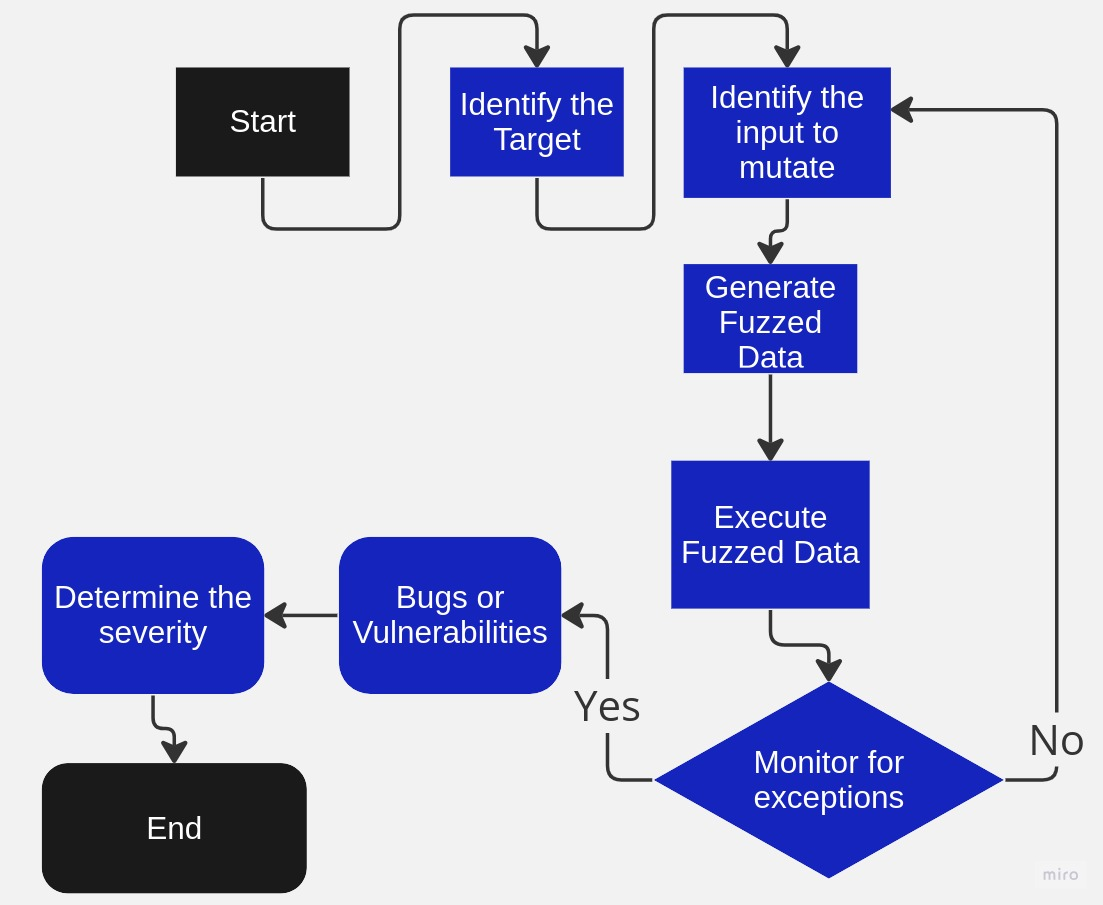
\includegraphics{fuzzy_testing_phases_1}}
        \caption{Fuzzing Stages~\cite{segedyfuzz}~\cite{9742291}}\label{fig:fuzzy_testing_phases_1}
\end{figure}

Overall, the use of fuzzy testing provides a valuable approach to identifying potential
vulnerabilities in software systems. By generating many test cases with both
valid and malformed data, fuzzing techniques can expose weaknesses in software that may not be
detected through traditional testing methods. Additionally, the analysis of the results of the
fuzzing process enables software developers to identify and address potential security issues
before they can be exploited by malicious actors.

\subsection{History and Evolution of Fuzzy Testing}
The term ``fuzzing'' or ``fuzz testing'', although a relatively recent addition
to the lexicon of automation techniques, was first introduced by Barton Miller
in 1988 as part of a class project~\cite{takanen2009fuzzing}. Initially,
fuzzing was perceived as an ad-hoc or random testing method used within
mission-critical applications~\cite{WhatisaM24:online}. Over time, however, it
has developed into a specialized technique for the automated generation and
testing of extensive sets of input values for software systems~\cite{bohme2020fuzzing}.

The advent of the first open-source fuzz testing framework in 2007~\cite{takanen2009fuzzing}
marked a significant evolution in formalizing fuzzing as an approach to software testing.
This led to the creation of a myriad of additional frameworks and tools, expanding the
application of fuzz testing across a diverse set of software systems.

Since its inception, fuzzing has considerably broadened its capacities.
Initially, it was utilized mainly to uncover memory corruption bugs. However,
as discussed by \Citeauthor{bohme2020fuzzing}, its functionality has
evolved over time to include the identification of a diverse range of
software vulnerabilities~\cite{bohme2020fuzzing}. \Citeauthor{takanen2009fuzzing} and \Citeauthor{vidas2019fuzzy}
explain that the flexibility and customization capabilities of modern fuzzing
frameworks enable their application across various software layers,
making fuzzing a potent tool for identifying potential weak spots in
software systems~\cite{takanen2009fuzzing}.

Fuzzing techniques have evolved beyond mere bug detection, becoming an essential
tool for vulnerability discovery and, potentially, exploitation.
As indicated by \citeauthor{beaman2022fuzzing}, fuzzing can be
systematically applied to uncover software vulnerabilities, which
may subsequently become exploitable avenues for security
attacks~\cite{beaman2022fuzzing}. The subsequent section, referenced as
Section~\ref{par:success_of_fuzzing}, describes the accomplishments and
vulnerabilities revealed by fuzzing techniques over time.

\subsection{Successes Of Fuzzing}~\label{par:success_of_fuzzing}
Fuzzy testing has proven to be an extremely effective technique since its inception in the
late 1980s, discovering long-standing bugs, vulnerabilities, and thereby improving the
quality and security of software. Over the years, a wide range of applications,
as shown in Section~\ref{par:target_categories}, have been successfully fuzzed,
revealing critical security vulnerabilities that could have been exploited by malicious actors.

The Table:~\ref{tab:vulnerabilities_examples} showcases examples of vulnerabilities discovered by
fuzzing tools and the affected components.

\begin{table}[h!]
\centering
\begin{tabularx}{\textwidth}{@{}>{\raggedright\arraybackslash}p{2cm}>{\raggedright\arraybackslash}p{3cm}X@{}}
\toprule
\textbf{Fuzzing Tool} & \textbf{CVE ID} & \textbf{Description and Affected Component} \\
\midrule
AFL & CVE-2014-0160 & Heartbleed vulnerability in OpenSSL, affecting the TLS heartbeat extension~\cite{durumeric2014matter} \\
\addlinespace
AFL & CVE-2014-6271 & Shellshock vulnerability in the Bash shell, allowing remote code execution~\cite{shetty2018shellshock} \\
\addlinespace
libFuzzer & CVE-2016-1839  & Heap buffer overflow in ImageIO, affecting image decoding in macOS and iOS \\
\addlinespace
syzkaller & CVE-2017-2636  & Double fetch vulnerability in the Linux kernel, allowing privilege escalation~\cite{wang2017double} \\
\addlinespace
go-fuzz & CVE-2016-3959  & Denial of service vulnerability in Go's standard library, affecting the HTTP/2 implementation \\
\addlinespace
Honggfuzz & CVE-2017-15650  & Heap buffer overflow in Poppler, affecting PDF rendering~\cite{haller2013dowsing} \\
\bottomrule
\end{tabularx}
\caption{Examples of Vulnerabilities Discovered by Fuzzing Tools}
\label{tab:vulnerabilities_examples}
\end{table}

%\pagebreak

%\clearpage
The Table:~\ref{tab:bugs_found_overview} provides a broader overview of the number of bugs found by
different fuzzing tools in various projects.

\begin{table}[h!]
\centering
\begin{tabularx}{\textwidth}{@{}>{\raggedright\arraybackslash}p{1cm}>{\raggedright\arraybackslash}p{2cm}>{\raggedright\arraybackslash}p{3cm}X@{}}
\toprule
\textbf{Year} & \textbf{Organization/Researchers} & \textbf{Fuzzing Tool/Project} & \textbf{Achievements} \\
\midrule
1999 & OUSPG & PROTOS & Found security vulnerabilities in Voice over IP (VoIP) implementations~\cite{roning1999protos} \\
\addlinespace
2007 & Microsoft & SAGE & Found critical vulnerabilities in Windows and Office products and had a remarkable impact at Microsoft~\cite{godefroid2012sage} \\
\addlinespace
2010 & Adobe & NA & Vulnerabilities uncovered by fuzzing in Adobe Flash, Reader, and Acrobat~\cite{AdobeFla64:online} \\
\addlinespace
2016 & ForAllSecure & Mayhem & Competed in DARPA's Cyber Grand Challenge, identified, patched vulnerabilities in real-time~\cite{“Mayhem”62:online} \\
\addlinespace
2019 & Microsoft & Project OneFuzz & Used for fuzzing Azure Cloud~\cite{GitHubmi60:online} \\
\addlinespace
2023 & Cross platform & AFL & More than 2000 bugs found in open source projects, including OpenSSL, PHP, Python, and others~\cite{american20:online} \\
\addlinespace
2023 & Cross-platform & libFuzzer & More than 1000 bugs found in Chromium, OpenSSL, LibreOffice, and other projects~\cite{libFuzze17:online} \\
\addlinespace
2023 & Linux kernel developers & syzkaller & More than 800 bugs found in the Linux kernel~\cite{syzkalle20:online} \\
\addlinespace
2023 & Go community & go-fuzz & 200+ bugs found in Go programming language and related projects~\cite{GitHubdv6:online} \\
\addlinespace
2023 & Cross-platform & Honggfuzz & Bugs found in various projects, including Google's Android and Chrome, and others~\cite{GitHubgo17:online} \\
\addlinespace
2023 & Facebook & Facebook's Sapienz & Automated testing of Android apps, leading to crash fixes and improvements~\cite{SapienzI13:online} \\
\addlinespace
2023 & Google & ClusterFuzz & More than 25000 bugs found in Google and Chrome~\cite{ClusterF78:online} \\
\addlinespace
2023 & Google & OSS-Fuzz & 36,000+ bugs in over 550 open source projects~\cite{ClusterF78:online} \\
\bottomrule
\end{tabularx}
\caption{Overview of Bugs Found by Fuzzing Tools in Various Projects}
\label{tab:bugs_found_overview}
\end{table}

%\clearpage

The Table:~\ref{tab:embedded_fuzzing_success} includes fuzzing success in embedded systems and IoT devices
specifying whether the fuzzing tools are open-source or closed-source:

\begin{table}[h!]
\centering
\begin{tabularx}{\textwidth}{@{}>{\raggedright\arraybackslash}p{0.5cm}>{\raggedright\arraybackslash}p{1.5cm}>{\raggedright\arraybackslash}p{3.8cm}X>{\raggedright\arraybackslash}p{1.2cm}@{}}
\toprule
\textbf{No.} & \textbf{Fuzzing Tool} & \textbf{Target Systems} & \textbf{Achievements} & \textbf{Source} \\
\midrule
1 & AFLNet & FTP, HTTP, and SMTP implementations in IoT devices & Uncovered vulnerabilities and improved security in IoT devices\cite{lin2020aflnet} & Open-source \\
\addlinespace
2 & IoTcube & IoT devices including smart home appliances, medical devices, and industrial IoT devices & Identified and addressed security issues in IoT devices\cite{kim2019iotcube} & Closed-source \\
\addlinespace
3 & FirmFuzz & Firmware in IoT devices including IP cameras and routers & Discovered 7 previously undisclosed vulnerabilities across 6 different devices\cite{srivastava2019firmfuzz} & Open-source \\
\addlinespace
4 & FUZZY & Zigbee implementations in IoT devices & Identified new security vulnerabilities in Zigbee, a widely used wireless communication protocol for IoT devices\cite{vidas2019fuzzy} & Closed-source \\
\addlinespace
5 & Atheris & Python programs, including embedded systems using MicroPython & Detected various types of vulnerabilities, such as buffer overflows and memory leaks, in Python-based embedded systems\cite{atheris2020} & Open-source \\
\bottomrule
\end{tabularx}
\caption{Fuzzing Success in Embedded Projects}
\label{tab:embedded_fuzzing_success}
\end{table}

%\clearpage

\subsection{Why, How and What to Fuzz}

Fuzzing provides significant insights into the security, robustness,
and resilience of software systems, especially those that interact with inputs
from untrusted sources. While it does not make any guarantees about the
reliability of inputs or transforms an untrusted source into a trusted one,
it helps identify problematic inputs that could cause the software system to
crash or behave
unexpectedly~\cite{bohme2020fuzzing}~\cite{beaman2022fuzzing}~\cite{vidas2019fuzzy}~\cite{WhatisFu63:online}.

It's crucial to emphasize that fuzz testing doesn't necessarily affirm the
correctness of complex software programs. Instead, it contributes to the
understanding of the system's behavior under diverse and unexpected input
conditions. Particularly for software playing a critical role in larger
systems or applications, fuzz testing can highlight unforeseen
issues~\cite{fuzzinga40:online}~\cite{demott2006evolving}~\cite{WhatisFu63:online}.

Moreover, fuzz testing aids in assessing the software system's stability under
stress. By exposing the software to high volumes of varied inputs, this
technique can identify potential performance or stability issues, arising
from heavy usage or stress conditions~\cite{demott2006evolving}.

However, it's important to understand that fuzzing is not a panacea for
all software flaws. It's a specialized tool aimed at discovering errors
and vulnerabilities that might not directly relate to the software's
requirements or intended functionalities. While it's effective at uncovering
specific issues like memory leaks~\cite{shahriar2014testing},
address corruptions~\cite{muench2018you}, and buffer overflows~\cite{godefroid2020fuzzing},
it should complement other types of testing such as functional, unit,
integration, and system testing, rather than replace
them~\cite{pietikainen2016steps}~\cite{UnitTest25:online}~\cite{WhatisFu63:online}.

To leverage fuzzing effectively, careful planning is essential to identify
\gls{fuzz_target} for testing. Notably, identifying and defining entry points
for fuzzing in large and complex applications can be challenging but essential.
These entry points, including file inputs, network inputs, and command
line inputs, help fuzz testers concentrate their efforts on the areas
most susceptible to potential issues~\cite{oehlert2005violating}.
Thus, the meticulous selection of
fuzz testing targets is instrumental to the test's success, underpinning
thorough testing of the most vulnerable software components.

Below given examples applications targets where fuzzing has been successful~\cite{fuzzingw44:online}.\label{par:target_categories}

\begin{itemize}
        \item Databases: SQLite~\cite{fu2022griffin}
        \item Text editors: VIM~\cite{FuzzingV8:online}, OpenOffice~\cite{Presenta60:online}
        \item Media codecs: audio, video, raster and vector images~\cite{thiel2008exposing}~\cite{rhodenfuzzing}
        \item Linux OS kernels, drivers~\cite{schumilo2017kafl}~\cite{corina2017difuze}
        \item Parsers: xml, pdf~\cite{wang2017skyfire}
        \item Crypto libraries: OpenSSL~\cite{opensslR89:online}, LibreSSL~\cite{GitHubli9:online}
        \item Browsers: Chrome~\cite{Fuzztest23:online}, Firefox~\cite{Fuzzing—21:online}
        \item Network protocols~\cite{GitHubnc82:online}, scanners~\cite{SnapFuzz27:online}
\end{itemize}


\section{Fuzzing Process, Components, and Various Approaches}\label{sec:fuzzing_methods}
Fuzzing, a dynamic software testing technique, plays a crucial role in enhancing
software reliability and security by detecting concealed bugs and
vulnerabilities. Its importance has grown in tandem with the increasing
complexity and pervasiveness of software systems, making it a prominent
field of academic and practical interest. This section provides an exhaustive
exploration of the fuzzing process, including its various stages, the evolution
of its techniques, and the methodologies employed.

\subsection{Test Case Generation: From Basic to Advanced Techniques}
The process of fuzzing begins with the generation of numerous inputs
designed to provoke the program's failure. These inputs can be in various forms,
including different file formats, binary executables, or network commands
~\cite{mcnally2012fuzzing}~\cite{bohme2020fuzzing}~\cite{manes2019art}.
Creating broken inputs that can trigger a program to fail is a
significant challenge. This is addressed through mutation-based
~\cite{miller2007analysis}~\cite{lyu2022ems} and
generation-based generators~\cite{pang2023generation}.

Mutation-based fuzzing represents an evolution from primitive fuzzing techniques
that relied heavily on generating inputs using random bytes.
This mutation-based fuzzing technique employs existing input data,
referred to as a test \gls{corpus}, and modifies it to produce new test data~\cite{miller2007analysis}.
These mutation algorithms can vary significantly, with some utilizing
stochastic modeling to concentrate mutations on specific parts of the input~\cite{lyu2022ems}~\cite{miller2007analysis}.

Generation-based generators, conversely, create entirely new inputs
for fuzzers, serving as a crucial tool in the
fuzzing process~\cite{li2018fuzzing}~\cite{miller2007analysis}~\cite{wang2017skyfire}.

\subsection{Execution and Monitoring: Coverage-Guided Fuzzing and Sanitizers}
After generating the inputs, the test cases are fed into the program, and the
fuzzing process continues until a program crash or hang occurs. This
stage involves monitoring crashes and exceptions using tools like
sanitizers~\cite{GitHubgo55:online}~\cite{osterlund2020parmesan}, which can detect specific system signals,
crashes, and other violations.

\subsection*{Sanitizers}

Sanitizers play a vital role in the fuzzing process, aiding in the detection of
bugs that may not necessarily lead to a crash. However, their operation is
resource-intensive, increasing both CPU~\cite{WhatisaC78:online} and
RAM~\cite{WhatisRA11:online} usage. Thus, the application of
sanitizers should be judiciously managed to prevent excessive resource consumption.

\begin{itemize}

\item \textit{Address Sanitizers (ASAN)~\cite{AddressS43:online}:} These tools
are indispensable for uncovering vulnerabilities linked to memory corruption,
such as use-after-free, NULL pointer dereferences, and buffer overflows~\cite{haller2013dowsing}.

\item \textit{Memory Sanitizers (MSAN)~\cite{MemorySa64:online}:} They are designed
to detect unauthorized read accesses to uninitialized memory, such as when a local
variable is defined and read prior to being set~\cite{stepanov2015memorysanitizer}.

\item \textit{Undefined Behavior Sanitizers (UBSAN)~\cite{Undefine50:online}:} These sanitizers are instrumental
in pinpointing instances of undefined behavior as per the C and C++ standards,
such as when the outcome of an operation exceeds the permissible limit of a data type.
\end{itemize}

Coverage-guided fuzzing~\cite{jaaskela2016genetic} is a subset of feedback-based
fuzzing that specifically uses code coverage as its feedback mechanism. It represents another integral element of
the execution and monitoring phase. This technique involves monitoring the extent and
sections of the \acrshort{sut} that are traversed by the inputs during the
fuzzing campaign. Compiler instrumentation, employed by fuzzers like
AFL/AFL++~\cite{257204} or libFuzzer~\cite{libFuzze17:online}, is commonly
used to collect this data. External function calls are inserted at
specific points during the compilation process to relay information to the fuzzer each
time an edge or block is reached~\cite{libFuzze17:online}~\cite{bohme2016coverage}~\cite{257204}.


The Figure:~\ref{fig:feedback-based-fuzzing} depicts a simple visual representation of the
feedback based fuzzing.

% \begin{figure}[ht]
% \centering
% \AltText{Feedback Based Fuzzing}{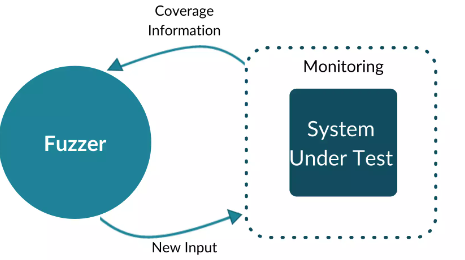
\includegraphics[width=8.5cm, height=5.5cm]{feedback-based-fuzzing}}
% \caption{Feedback Based Fuzzing\cite{TheMagic36:online}\cite{LucianoR49:online}}\label{fig:feedback-based-fuzzing}
% \end{figure}

\begin{figure}[h]
        \centering
        \adjustbox{width=\textwidth}{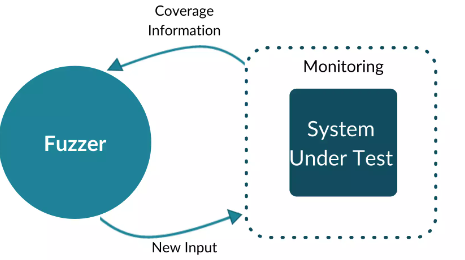
\includegraphics{feedback-based-fuzzing}}
        \caption{Feedback Based Fuzzing~\cite{TheMagic36:online}\cite{LucianoR49:online}}\label{fig:feedback-based-fuzzing}
\end{figure}

\subsection{Analysis: Discovering and Filtering Bugs}
The analysis stage is centered on uncovering the underlying cause of issues
unearthed during the monitoring phase. This stage comprises the bug
detector~\cite{liang2018fuzzing}~\cite{bekrar2012taint}, a vital element in fuzzers
aimed at pinpointing potential bugs,
and the bug filter~\cite{peng2018t}~\cite{bekrar2012taint}~\cite{chen2013taming},
which segregates non-security related bugs
from the aggregate of reported bugs. The bug detector aggregates and scrutinizes the
stack traces resulting from the crashes and errors induced by the test
inputs, while the bug filter aids in distilling these results to give precedence
to security-centric bugs.

\subsection*{Visibility in Fuzzing}

The term ``Visibility'' in the context of fuzzing refers to the extent of information about the
\acrshort{sut} accessible to the fuzzer during runtime. There exist three primary levels of visibility in
fuzzing: Blackbox~\cite{godefroid2007random}~\cite{manes2019art},
Graybox~\cite{canakci2021directfuzz}~\cite{li2018fuzzing}, and
Whitebox~\cite{godefroid2008automated}~\cite{godefroid2007random}~\cite{godefroid2008grammar} fuzzing,
each proffering varying degrees of access to the source code of the \acrshort{sut}.

The amalgamation of these methodologies—mutation-based~\cite{lyu2022ems}~\cite{miller2007analysis}
test case generation, coverage-guided~\cite{jaaskela2016genetic} execution and monitoring, in-depth bug analysis,
and the consideration of visibility levels—positions fuzzing as a formidable instrument
in bolstering the overall software quality and security. By diagnosing and
rectifying the root cause of software bugs and vulnerabilities, developers
can stymie the potential exploitation of these flaws by attackers.

The Figure:~\ref{fig:general_process_fuzzing} offers a visual representation of the
fuzzing process and its dependencies.

% \begin{figure}[ht]
% \centering
% \AltText{General Process Fuzzing}{\includegraphics[width=12.1cm][height=20.1cm]{general_process_fuzzing}}
% \caption{General Process Fuzzing\cite{liang2018fuzzing}.}\label{fig:general_process_fuzzing}
% \end{figure}

% \begin{figure}[ht]
% \centering
% \AltText{General Process Fuzzing}{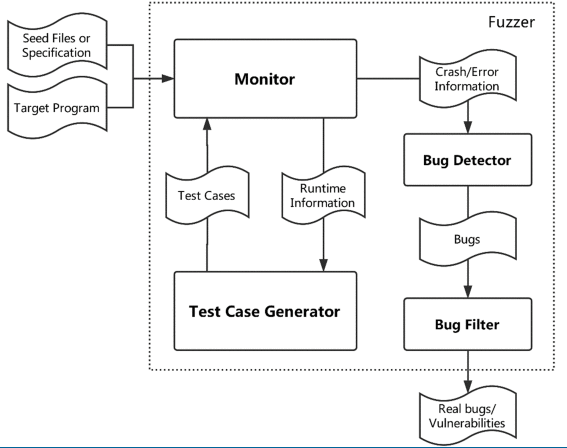
\includegraphics[width=14.5cm, height=20.5cm]{general_process_fuzzing}}
% \caption{General Process Fuzzing\cite{liang2018fuzzing}}\label{fig:general_process_fuzzing}
% \end{figure}

\begin{figure}[h]
        \centering
        \adjustbox{width=\textwidth}{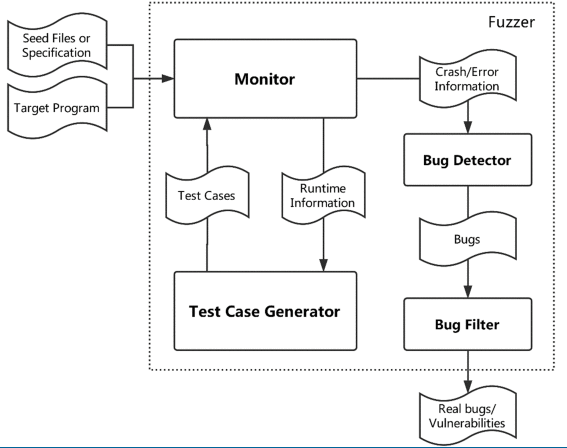
\includegraphics{general_process_fuzzing}}
        \caption{General Process Fuzzing~\cite{liang2018fuzzing}}\label{fig:general_process_fuzzing}
\end{figure}

As the \gls{fuzz_target} of a fuzzing test, the \acrshort{sut}, typically a binary program,
is meticulously scrutinized by fuzzers. The generated inputs for the fuzzing process,
derived from either mutation-based or generation-based methods, comprise a mixture of valid and
invalid inputs that pass initial validation but may still trigger bugs. The process is dynamic
and continuously evolving, with ongoing research aimed at improving and automating the various
stages, from input generation to bug detection and filtering.
%\clearpage


% \section{Classification of Fuzzing Methods}\label{sec:fuzzing_methods}
% Fuzzing tools and methods are classified into three main categories: gray-box, white-box and
% black-box fuzzing.

% \subsection{White-Box Fuzzing Method}

% White-box fuzzing is a systematic technique for enumerating different interesting paths in a
% program by using program analysis and constraint solvers. It relies on the internal logic
% of the target program and is based on the technique called \textit{symbolic execution}\cite{cadar2013symbolic}.
% This method was proposed to overcome the limitations of black-box fuzzing and was first
% \Citeauthor{godefroid2008automated}. To scan through the target program, white-box fuzzing uses
% a search technique called coverage-maximizing heuristic search
% algorithm\cite{godefroid2008automated}\cite{liang2018fuzzing}.

% Before starting the fuzzing process, white-box fuzzing requires the necessary information
% from the target program to generate the inputs. It collects all the conditional paths of the target
% program by applying \acrlong{smt} formulas. For example, it uses the formula
% \begin{math}i[0] = 42 \land i[0] - i[1] > 7\end{math}, where \textit{i} is the set of inputs
% that traverse the target\cite{bohme2021fuzzing}. The path condition is then calculated and mutated
% and sent to a constraint solver to generate new paths and skip the blocks.
% The main goal of white-box fuzzers is to reach the maximum execution paths and requirements.


% One of the advantages of white-box fuzzing is that it can cover maximum coverage by generating
% better and more interesting test cases. However, numerous execution paths can lead to stability and
% compatibility issues in real-world software\cite{lomeli2022security}\cite{liang2018fuzzing}.
% Some existing white-box fuzzers are SAGE\cite{godefroid2012sage}, KLEE\cite{cadar2008klee},
% BitFuzz\cite{caballero2010input}.\newline

% \subsection{Black-Box Fuzzing Method}
% Black-box testing method involves generating inputs to test the target program without any
% internal knowledge or specifications. The fuzzing process begins by randomly mutating
% the valid inputs or generating new inputs. Examples of mutation data include flipping random bits
% and bytes in a seed file, byte copies, and removal\cite{jaaskela2016genetic}.
% Generational-based approaches utilize grammar and input-specification knowledge\cite{kim2013automatic}.

% The fuzzing process ends after a predefined time has been exhausted. Popular black-box fuzzers
% include Peach\cite{PeachFuz35:online}, Trinity\cite{GitHubke76:online} and
% Funfuzz\cite{GitHubMo73:online}.\newline

% \subsection{Gray-Box Fuzzing Method}
% The combination of black-box and white-box fuzzing utilizes \textit{code instrumentation}
% to provide feedback and obtain code coverage of the target program during runtime\cite{bohme2021fuzzing}.
% This approach employs genetic algorithm mutation strategies to generate new inputs which serve as
% new control locations to cover additional coverage paths. Feedback received from the coverage
% enables the fuzzers to reach more coverage, including tracing the taint data flow, in a method known
% as gray-box \textit{taint-analysis}\cite{bekrar2012taint}.

% To detect bugs and vulnerabilities, assertions are injected by sanitizers into the target program.
% Unlike the white-box method, the gray-box method utilizes runtime information to generate test cases.
% Some well-known gray-box fuzzers include AFL++\cite{257204}: a fork
% of \gls{afl}\cite{GitHubgo92:online}, LibFuzzer\cite{libFuzze17:online} and Honggfuzz\cite{GitHubgo89:online}.\newline

% \subsection{Choose a Fuzzing Method}
% In software testing, a `bug' refers to a defect in the software logic that causes unexpected or
% incorrect output. The primary objective of fuzz testing is to identify and eliminate such bugs
% in a system. In order to achieve this objective, selecting an appropriate fuzzing target is of
% utmost importance. While black-box fuzzers are simple and lightweight, they may not be capable
% of achieving high levels of code coverage and are more effective in uncovering `shallow`
% bugs. On the other hand, white-box and gray-box fuzzers are adept at detecting  `hidden' bugs
% that are difficult to identify. Although the implementation of these fuzzers is more complex
% and time-consuming, they offer comprehensive and in-depth testing capabilities.

% When considering fuzz testing methods, two important factors to consider are precision and efficiency,
% as well as the quality of the results. A `dumb' fuzzer simply mutates a valid input by
% randomly changing some bytes, while a `smart' fuzzer generates inputs from scratch.
% The black-box fuzzing approach is known for its precision and efficiency, while the white/gray
% box methods tend to produce higher quality results. Careful consideration of these factors is
% essential when selecting an appropriate fuzz testing method for a given software system.

% The two factors are:
% \begin{enumerate}
%         \item Time and Budget
%         \item Input format of the target program e.g, network protocol, compiler
% \end{enumerate}

% \section{Implementing the Art of Fuzzing}
% As per the section \hyperref[sec:fuzzing_methods]{Classification of Fuzzing Methods} below questions\cite{liang2018fuzzing}
% should be considered when building and implementing fuzzing with fuzzers.

% \begin{itemize}
%         \item How to do seed selection and generation.
%         \item What makes a good \gls{fuzz_target} and how to validate the inputs.
%         \item What to consider with the test cases which indicates crashes.
%         \item How to make good use of information during the runtime.
%         \item How can we achieve scalability improvements.\newline
% \end{itemize}

% \subsection{Generation and Selection of Seed}

% In the field of fuzz testing, the term \textit{seed corpus} denotes an assortment
% of representative input files that a target program is designed to process.
% The composition of the seed corpus can profoundly influence the efficacy and efficiency
% of the fuzzing process, emphasizing the importance of its selection for
% maximizing test coverage\cite{herrera2021seed}.

% Striving for high coverage implies the goal to activate and evaluate as
% many code paths as possible within the target program during the fuzzing process.
% While 100\% coverage represents a theoretical ideal, practically achieving this
% level of thoroughness is rare due to the intricate and expansive nature of
% modern software. Nevertheless, aiming for high coverage substantially enhances
% the probability of revealing concealed bugs and vulnerabilities, thus providing
% a comprehensive evaluation of the system's reliability and security\cite{godefroid2012sage}.

% The size of the seed corpus necessitates a careful balancing act between file
% size and coverage. While larger seed files may offer greater potential for
% coverage, they consume more computational resources and processing time. Smaller
% seed files, processed more rapidly, might not deliver the same level of coverage.
% Therefore, if a smaller seed file yields similar coverage to a larger one, its
% usage is preferable for improved testing
% efficiency\cite{liang2018fuzzing}\cite{jurczyk2016effective}. Nonetheless,
% in scenarios with ample storage capacity—either physical or cloud—larger seed
% files can be utilized, often compressed to conserve space without compromising
% the comprehensive representation of potential program inputs\cite{liang2018fuzzing}.

% The selection of the seed corpus typically precedes the fuzzing process,
% particularly crucial when employing a mutation-based fuzzer. This type of fuzzer
% requires an initial set of inputs or \textit{seed corpus} to commence testing.
% The quality of these initial seeds significantly influences the fuzzer's capacity
% to explore the program's state space and detect bugs\cite{miller2007analysis}.

% Moreover, a method for enhancing code coverage, as
% proposed by\Citeauthor{kim2011efficient}\cite{kim2011efficient},
% involves an in-depth analysis of binary file fields during fuzzing.
% This strategy entails tracking and evaluating stack frames, assembly codes,
% and registers to unearth potential new inputs that could augment coverage.

% In summary, the careful selection of a suitable seed corpus is a vital
% component of effective fuzz testing. The goal is to optimize coverage while
% considering the constraints of file size and storage capacity. Particularly in
% mutation-based fuzzing, a well-chosen seed corpus can lead to a more efficient and
% comprehensive exploration of the target program.


% \subsection{A Good Fuzz Target and Validation of Inputs}
% In the context of fuzz testing, the term `fuzz target' refers to the item being tested.
% This item can take many forms, such as a command line tool or a hardware device, and is
% characterized by its ability to accept inputs and provide results. The effectiveness of
% the fuzz testing process depends on the quality of the fuzz target and its ability to
% accurately represent the behavior of the real-world system or application being tested\cite{238602}.

% \subsubsection{A Good Fuzz Target}
% Below given is an example of a fuzz target written in C with \textit{LLVM libFuzzer}\cite{libFuzze17:online},
% \begin{minted}[linenos,frame=lines,baselinestretch=1.2,breaklines]{c}

% extern "C" int LLVMFuzzerTestOneInput (const uint8_t *Data, size_t Size) {
%         DoSomethingInterestingWithMyAPI(Data, Size);
%         return 0;  // Values other than 0 and -1 are reserved for future use.
% }

% \end{minted}

% The function \textit{LLVMFuzzerTestOneInput} of the fuzzer \textit{libFuzzer} takes two arguments,
% the address of the data to store and size. The API of the fuzz target is called in the next steps of
% fuzzing.

% It is crucial to keep the following aspects in mind when creating a fuzz target\cite{libFuzze17:online}\cite{257204}:

% \begin{itemize}
% \item The \gls{fuzzing_engine} needs to be designed so that it can execute the fuzz target multiple times within the same process, enhancing efficiency.
% \item The fuzz target should be able to handle a wide range of inputs, from valid to malformed and even empty inputs, increasing its robustness.
% \item An abrupt halt or unexpected exit from the fuzz target typically indicates a bug within the system. Thus, these instances warrant close monitoring.
% \item To expedite testing, the fuzz target's execution speed should be optimized. Furthermore, it should be designed to consume minimal memory, avoiding the risk of out-of-memory errors.
% \item If the fuzz target relies on a global state, it should be designed to avoid modifying it. For instance, the use of \textit{malloc()} could inadvertently modify the global state.
% \item To foster a culture of regular testing, the fuzz target should be integrated into a \textit{continuous integration} system.
% \item Consistent results are key in fuzzing. Consequently, the fuzz target should be deterministic, meaning that it should not rely on random factors that could lead to inconsistent outcomes.
% \item The fuzz target should be designed for speed as the fuzzing process requires multiple iterations. Therefore, its performance can significantly impact the testing speed.
% \item The memory consumption of the fuzz target should be kept minimal to avoid running into out-of-memory errors which could disrupt the testing process.
% \item It is essential to ensure the fuzz target is designed in a way that avoids conditions that could lead to timeouts and out-of-memory errors, thus ensuring smooth and uninterrupted testing.
% \end{itemize}

% \subsubsection{Input Validations}
% Fuzzing offers the main advantage of generating test cases quickly. However, when the fuzz target
% being tested has input validations, the generated test cases may not be useful. Hence, it is
% crucial to exercise caution when creating test cases in such scenarios.

% \textbf{Integrity Validation:}
% Integrity validation is a crucial aspect of maintaining data integrity in various inputs
% such as file formats and network protocols. To ensure the integrity of the data,
% checksum mechanisms are used, which provide validation at both the sending and receiving ends.
% In this regard, a fuzzer named \textit{TaintScope}, developed by \citeauthor{wang2010taintscope},
% is used to mutate the hot bytes in the input, which helps in generating new test cases. However, to pass the
% integrity validation, the checksum is reverted to its original state. This approach enables
% the detection of vulnerabilities that might arise in the process of transmitting data,
% which could compromise the integrity of the system\cite{wang2010taintscope}.

% \textbf{Format Validation:}
% Fuzz targets such as Android devices, compilers, and interpreters have format requirements that
% must be met by inputs in order to be accepted for testing. However, in cases where inputs
% do not conform to these formats, they are rejected by the system. To avoid format-based validation,
% a \textit{Grammar}-based solution can be employed. For instance, \Citeauthor{cao2015towards},
% developed a scanner for fuzz targets on Android devices, which is capable of evading the
% initial format validation and allowing the fuzz testing process to continue without
% interruption\cite{cao2015towards}.

% \textbf{Environment Validation:}
% Environment validation is a crucial aspect of testing, which checks the validity of configurations,
% runtime status, and other environmental factors. Fuzzing tools, such as FuzzDroid\cite{rasthofer2017making},
% utilize a combination of static and dynamic analysis to generate an Android runtime environment.
% The tool employs a search-based algorithm to identify potential vulnerabilities, which helps in
% enhancing the overall security of the system. Through this approach, FuzzDroid can effectively
% identify and address issues related to syntactic and semantic validity, ultimately improving the
% reliability and performance of the system.


% \textbf{Input Coverage:}
% Achieving high input coverage is critical to uncovering vulnerabilities in a target system.
% Various techniques have been proposed to improve the input coverage of a fuzzer.
% One such tool is the \textit{semi-valid coverage (SVCov)} tool, proposed by  \Citeauthor{tsankov2013semi},
% SVCov helps increase the existing input coverage by generating inputs that are close to
% valid inputs but still contain errors or faults that can trigger bugs in the system under test\cite{tsankov2013semi}.

% Another technique to enhance input coverage is through the use of specialized fuzzers such as \textit{Artfuzz},
% which was proposed by \Citeauthor{chen2016dynamically}. Artfuzz is designed to find non-crash buffer overflow
% vulnerabilities by identifying inputs that can trigger buffer overflows but do not cause the system to crash.
% By uncovering such vulnerabilities, Artfuzz helps improve the security of the target system\cite{chen2016dynamically}.

% \subsubsection{Isolating Crashes and Test Cases}
% Fuzzing often causes crashes in the target systems. These crashes can be huge in numbers and often
% takes a large amount of time for analyzing. Due to time and budget often the most priority bugs get
% fixed by the developers. Therefore, it is really important for the testers to isolate or filter
% the test inducing crashes and take the most useful test cases into account.

% \Citeauthor{chen2013taming} introduced a ranking based to isolate the crashes and test cases\cite{chen2013taming}.
% In this method, the test cases which can cause bugs, and they are different in nature are ranked accordingly.
% There are other methods for isolating the crashes such as clustering methods, differentiating the crashes based
% on their uniqueness and debug information. The stack traces play an important role in determining the uniqueness
% of the test cases and therefore need to recorded while doing the fuzzing. Another simpler way to determine the
% uniqueness is to trace the execution path. Fuzzers like AFL\cite{GitHubgo92:online} determines a crash is unique
% when it does not find the execution path. The uniqueness helps in isolating the crashes, the outputs and saves
% time when analyzing them. Trimming of the test cases is another method of isolating the crashes and test cases.
% A large size test case can take more time to execute and then more time for analysis. In mutation based fuzzers,
% in which the test cases are developed and mutated during the run time usually fall into this category. Hence, trimming
% of the test cases is needed from time to time while fuzzing and which can improve the overall efficiency. Trimming
% is usually done by removing the identical data-blocks which can not influenced the execution path anymore
% by comparing them with the original one.

% \subsubsection{Runtime Information During Fuzzing}
% To get code coverage and data flow which are runtime information,  symbolic execution and dynamic
% analysis techniques are used. Although these techniques help in finding the `hidden' bugs, these smart
% fuzzing techniques are low in efficiency.


% Path Explosion is one of the biggest problem in symbolic execution during fuzzing run time. A conditional branch
% in any target program can have a numerous execution paths and this can lead to Path Explosion.
% \Citeauthor{godefroid2007compositional} proposed to have \textit{function summaries} in low level
% functions. This can lead to less number of execution paths as the higher level functions can
% reuse them\cite{godefroid2007compositional}. Heuristic search algorithms such as random path selection
% and automatic partial loop summarization help to find the most relevant paths\cite{liang2018fuzzing}.

% Complex programs can cause imprecision symbolic execution. Methods such as CUTE\cite{sen2005cute} helps
% in making the symbolic execution more cost effective.

% During the runtime, \textit{Undertainting} is another problem where without any direct assignment The
% variable is transferred. \Citeauthor{kang2011dta++} has proposed that to Undertainting, it is essential to
% neglect the input data flow if the input is tainted\cite{kang2011dta++}.


% \subsubsection{Isolating Crashes and Test Cases}

% Fuzzing frequently leads to numerous system crashes, which can be cumbersome and
% time-consuming to analyze. As a result of time and budget constraints,
% prioritization becomes crucial; hence, testers must effectively isolate
% and filter crash-inducing test cases. \Citeauthor{chen2013taming} proposed a
% ranking-based method to categorize these cases based on their bug-inducing
% capabilities and their distinctiveness\cite{chen2013taming}.

% Isolation of crashes can also be achieved through clustering methods,
% differentiating crashes based on uniqueness and debug information. Stack
% traces and execution path tracing are essential in determining the uniqueness
% of the test cases. For instance, AFL uses the absence of a pre-existing execution
% path to define the uniqueness of a crash\cite{GitHubgo92:online}.

% Trimming is another approach employed to optimize the fuzzing process. Large
% test cases, often generated in mutation-based fuzzers, could potentially slow
% down execution and analysis. To counter this, identical data-blocks that no
% longer influence the execution path are removed periodically, thereby enhancing
% overall efficiency.

% \subsubsection{Runtime Information During Fuzzing}

% Smart fuzzing techniques like symbolic execution and dynamic analysis are used
% to gather runtime information such as code coverage and data flow, although
% their efficiency can be limited. One significant challenge is path explosion,
% a phenomenon caused by the numerous execution paths stemming from a single
% conditional branch in the target program.

% \Citeauthor{godefroid2007compositional} suggested the use of `function summaries'
% for lower-level functions to reduce the number of execution paths, allowing
% higher-level functions to reuse them\cite{godefroid2007compositional}.
% Additionally, heuristic search algorithms like random path selection and
% automatic partial loop summarization help to identify the most relevant paths\cite{liang2018fuzzing}.


\section{Implementing the Art of Fuzzing}
Based on the classification of fuzzing methods delineated in
section \hyperref[sec:fuzzing_methods]{Classification of Fuzzing Methods},
several questions arise when constructing and implementing fuzzing with
fuzzers~\cite{liang2018fuzzing}:

\begin{itemize}
\item How to select and generate \gls{seeds}?
\item What characteristics define a good \gls{fuzz_target}, and how can one validate the inputs?
\item What considerations should be taken into account when dealing with test cases causing crashes?
\item How to effectively utilize information during runtime?
\item How to achieve scalability improvements?
\end{itemize}
The responses to these queries determine the effectiveness of fuzzing in
revealing hidden vulnerabilities, thereby enhancing the security and reliability of the target system.

\subsection{Generation and Selection of Seed}
The \gls{seeds} corpus in fuzz testing refers to a collection of representative input
files that the target program is designed to process. The seed corpus selection
can significantly influence the efficacy and efficiency of the fuzzing process,
emphasizing its importance for maximizing test coverage~\cite{herrera2021seed}.

In an ideal scenario, a fuzzer aims for 100\% coverage, seeking to activate and
examine as many code paths as possible within the target program. However, this
is rarely achieved due to the complex and large-scale nature of contemporary
software. Nonetheless, striving for high coverage significantly improves the
chances of uncovering hidden bugs and vulnerabilities, enhancing the evaluation
of system reliability and security~\cite{godefroid2012sage}.

The size of the seed corpus must be chosen with careful consideration of
its potential effect on coverage and computational resources. Larger seed files
may provide more coverage but consume more resources and time. If smaller seed
files can provide similar coverage to larger ones, they are typically preferred
for efficient testing~\cite{liang2018fuzzing}~\cite{jurczyk2016effective}.

The initial seed corpus is particularly crucial when using a mutation-based
fuzzer, which requires an initial set of inputs or \gls{seeds}. The quality of these
\gls{seeds} substantially influences the fuzzer's capacity to explore the program's
state space and detect bugs~\cite{miller2007analysis}. An efficient way of
enhancing code coverage, proposed by~\Citeauthor{kim2011efficient}, involves a
detailed analysis of binary file fields during fuzzing. This approach includes
tracking and evaluating stack frames, assembly codes, and registers to unearth
potential new inputs that could augment coverage~\cite{kim2011efficient}.

\subsection{A Good Fuzz Target and Validation of Inputs}
In the context of fuzz testing, the `fuzz target' is the item being tested.
This can be anything from a command line tool to a hardware device. The quality
of the \gls{fuzz_target} is crucial as it should accurately represent the behavior of
the real-world system or application being tested~\cite{238602}.

\subsubsection{A Good Fuzz Target}
Here is an example of a \gls{fuzz_target} written in C with
LLVM libFuzzer~\cite{libFuzze17:online}:

\begin{minted}[linenos,frame=lines,baselinestretch=1.2,breaklines]{c}

extern "C" int LLVMFuzzerTestOneInput (const uint8_t *Data, size_t Size) {
DoSomethingInterestingWithMyAPI(Data, Size);
return 0; // Values other than 0 and -1 are reserved for future use.
}

\end{minted}

In this case, the function \textit{LLVMFuzzerTestOneInput} takes two arguments,
the address of the data to store and its size. The API of the fuzz target is
called in subsequent steps of fuzzing. When creating a fuzz target, the
following aspects should be taken into account~\cite{libFuzze17:online}~\cite{257204}:

\begin{itemize}
\item The \gls{fuzzing_engine} should be designed to execute the fuzz target
multiple times within the same process to enhance efficiency.
\item The fuzz target should handle a wide range of inputs, from valid to
malformed and even empty, to increase robustness.
\item Any abrupt halt or unexpected exit from the fuzz target usually
signifies a bug within the system and warrants closer examination.
\item For faster testing, the fuzz target's execution speed should be
optimized. Moreover, it should consume minimal memory to avoid out-of-memory errors.
\item If the fuzz target relies on a global state, it should be
designed to avoid altering it.
\item Regular testing should be encouraged by integrating the fuzz
target into a continuous integration system.
\item The fuzz target should be deterministic to ensure consistent results.
\item It is crucial to optimize the performance of the fuzz target as the
fuzzing process requires multiple iterations.
\end{itemize}

\subsubsection{Isolating Crashes and Test Cases}
Fuzzing often results in many system crashes, which can be challenging and
time-consuming to analyze. Therefore, due to time and budget constraints, it's
important to isolate and filter crash-inducing test cases effectively. A
ranking-based method to categorize these cases based on their bug-inducing
capabilities and distinctiveness was proposed by~\Citeauthor{chen2013taming}~\cite{chen2013taming}.

Crashes can also be isolated through clustering methods, differentiating
crashes based on uniqueness and debug information. For example, AFL uses the absence
of a pre-existing execution path to define the uniqueness of a crash~\cite{GitHubgo92:online}.

\subsubsection{Runtime Information During Fuzzing}
Advanced fuzzing techniques, such as symbolic execution and dynamic analysis,
are used to gather runtime information, such as code coverage and data flow.
However, their efficiency can be limited due to challenges like path explosion,
a phenomenon caused by the multiple execution paths that stem from a single
conditional branch in the target program.

\Citeauthor{godefroid2007compositional} suggested using `function summaries'
for lower-level functions to reduce the number of execution paths. This allows
higher-level functions to reuse them~\cite{godefroid2007compositional}. Additionally,
heuristic search algorithms like random path selection and automatic partial
loop summarization help identify the most relevant paths~\cite{liang2018fuzzing}.

In summary, effective fuzzing implementation requires careful consideration of
various factors. The seed selection and generation, quality of the fuzz target,
test case management, use of runtime information, and scalability all play
significant roles in the process. Employing advanced techniques and maintaining
a clear focus on these aspects can optimize the fuzzing process and enhance its
ability to uncover hidden bugs and vulnerabilities in the target system.
\clearpage
% Fuzzing Tools And Fuzzers
 %if the chapter heading starts close to bottom of the page,
 %force a line break and remove the vertical vspace
\vspace{21.5pt}
\chapter{Embedded System, Challenges, Tools And Fuzzers}\label{sec:embedded_system}
In this chapter, the significant role of fuzz testing is highlighted as a method
to enhance the safety and dependability of embedded systems. It begins with a
comparative examination that differentiates traditional fuzz testing methods
from the specific challenges that arise when applying fuzz testing in the
context of embedded systems. This is followed by an extensive
examination of a selection of widely-used fuzzing tools and fuzzers,
assessing their operational competencies, user accessibility, efficacy, and
potential limitations. Key tools encompassed within this analysis include
AFL++~\cite{257204}, libFuzzer~\cite{libFuzze17:online}, ClusterFuzz~\cite{ClusterF90:online},
OSS-Fuzz~\cite{GitHubgo49:online}, FuzzTest~\cite{GitHubgo59:online}, and Atheris~\cite{atheris2020}. The chapter culminates with a meticulous
survey of relevant open-source initiatives and current research trajectories
within the field of fuzzing.

\section{Embedded System}
Embedded systems are specific types of computer systems built for specific tasks and
differ substantially from general-purpose computers~\cite{Top10Bes48:online}.
These integrated systems
consist of hardware, software, and sometimes mechanical parts, all engineered
for particular functions, on their own or as part of a bigger system.
Unlike general-purpose computers designed for multitasking, embedded systems
typically concentrate on performing a single task or a closely related set of
tasks~\cite{marwedel2021embedded}~\cite{yun2022fuzzing}~\cite{Introduc26:online}.

The Figure:~\ref{fig:Embedded_System} shows the different components of embedded systems.

% \begin{figure}[ht]
%         \centering
%         \AltText{Embedded System}{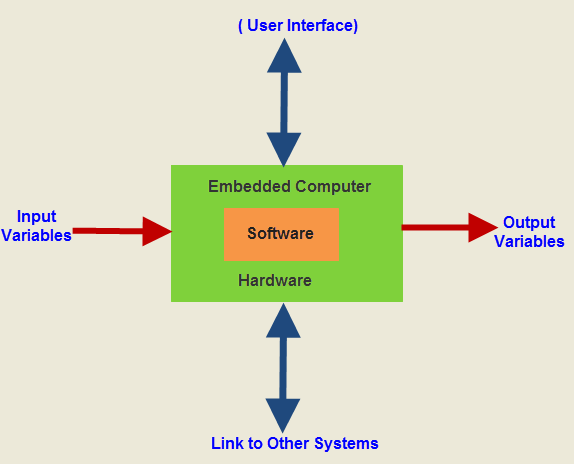
\includegraphics[width=8.5cm, height=8.5cm]{Embedded_System}}
%         \caption{Embedded System\cite{Introduc82:online}}\label{fig:Embedded_System}
% \end{figure}
\begin{figure}[h]
        \centering
        \AltText{Illustration of an Embedded System, showcasing its core components including the
        input/output interfaces, and connections to external devices.
        The diagram emphasizes the integration of hardware and software
        in a compact form for specific functionalities.}
        {\adjustbox{width=\textwidth}{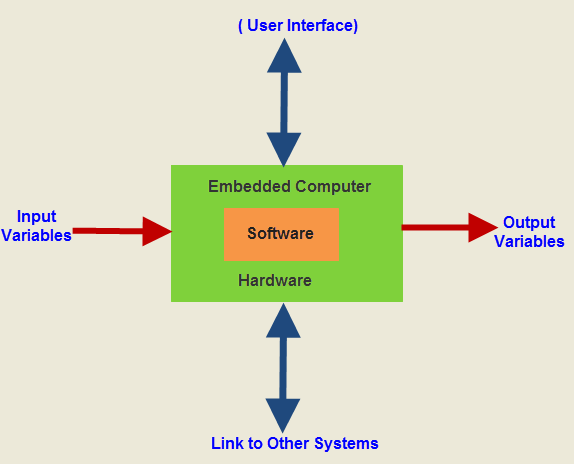
\includegraphics{Embedded_System}}}
        \caption{Embedded System~\cite{Introduc82:online}}\label{fig:Embedded_System}
\end{figure}

Just like conventional computer systems, embedded systems's core components
usually include a \gls{cpu}~\cite{WhatisaC78:online},
\gls{ram}, and input/output (I/O) interfaces. However,
embedded systems often lack user-friendly interfaces, and instead might
feature a minimal user interface or none at all~\cite{MainType35:online}.

Reflecting on the prior discussions of embedded systems and fuzzing in
Section~\ref{sec:sec_introduction} and Section~\ref{sec:sec_fuzzing} respectively,
this chapter explores further the significance and methodology of fuzzing
within the domain of embedded systems.

\subsection{Types of Embedded Devices}
There are several types of Embedded systems, such as standalone,
real-time, networked, and mobile systems~\cite{Classifi68:online}. These systems
play essential roles in various sectors, from consumer
electronics~\cite{andrae2010life} like digital watches~\cite{Whatisas39:online},
televisions, and cameras, to industrial machinery~\cite{thramboulidis2007soa},
medical equipment~\cite{jafari2007medical},
and automobiles~\cite{Automoti68:online}~\cite{li2003real}~\cite{MainType35:online}.

The Figure:~\ref{fig:types_of_embedded_devices} shows the different types of embedded devices.
% \begin{figure}[ht]
%         \centering
%         \AltText{Types of Embedded Devices}{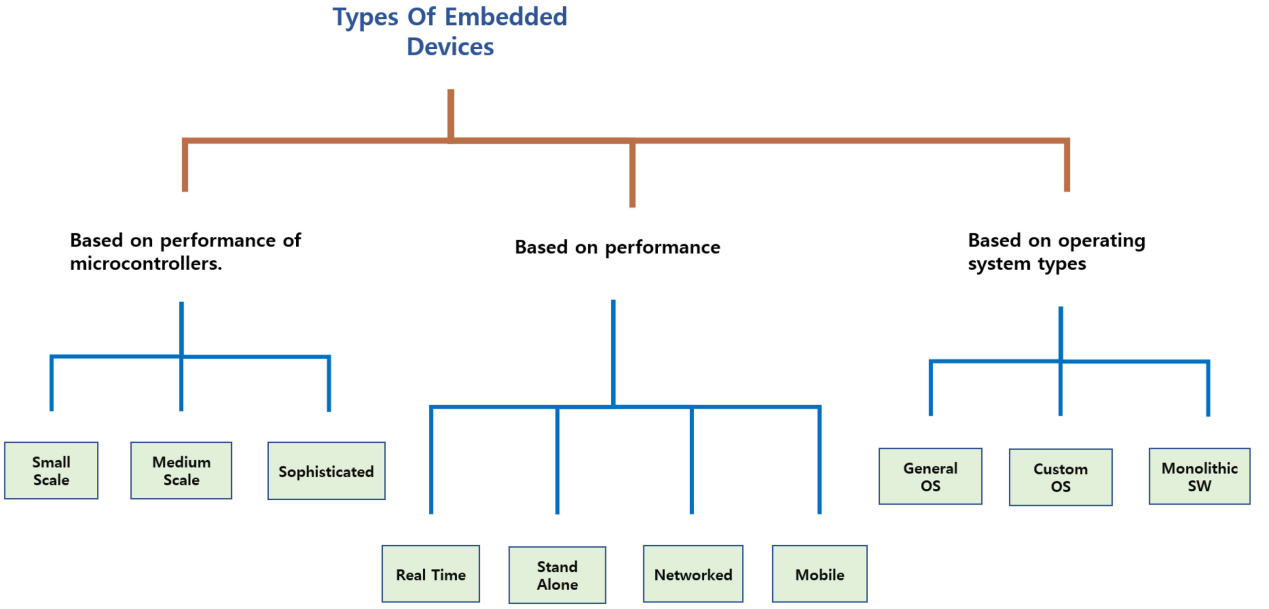
\includegraphics[width=8.5cm, height=8.5cm]{types_of_embedded_devices}}
%         \caption{Types of Embedded Devices\cite{yun2022fuzzing}\cite{WhatAreE30:online}}\label{fig:types_of_embedded_devices}
% \end{figure}

\begin{figure}[h]
        \centering
        \AltText{Diagram categorizing Types of Embedded Devices into three main
        groups: based on microcontrollers, performance levels, and operating
        system types.}
        {\adjustbox{width=\textwidth}{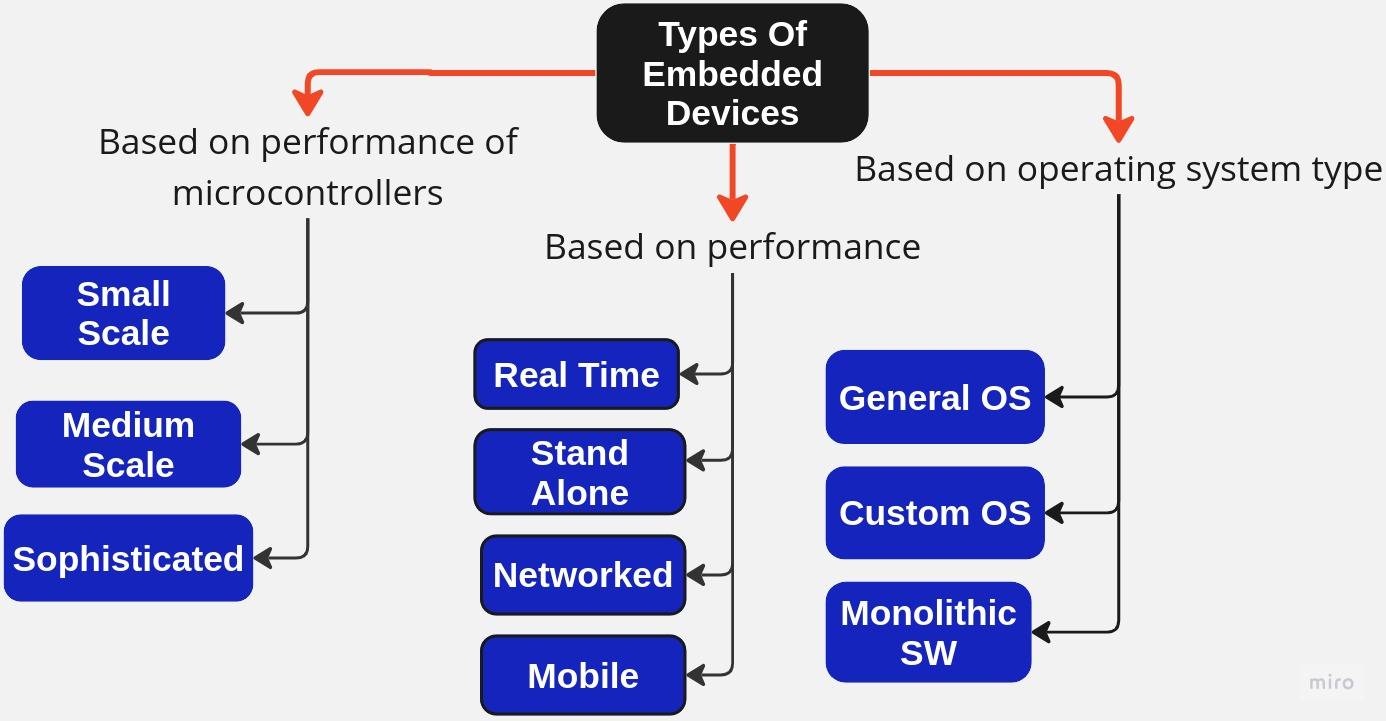
\includegraphics{illustration/types_of_embedded_devices.jpg}}}
        \caption{Types of Embedded Devices~\cite{yun2022fuzzing}~\cite{WhatAreE30:online}}
        \label{fig:types_of_embedded_devices}
\end{figure}

\subsection*{Standalone Devices:}

These devices constitute a subset of embedded systems functioning
independently, without the necessity for a host system. They process input data
within their own interfaces, producing outputs to control or drive attached
devices or to generate displays. These devices have found broad applicability in
various appliances due to their flexibility and efficiency. They often employ
lightweight user environments for
optimal performance~\cite{yun2022fuzzing}\cite{WhatAreE30:online}\cite{TypesofE31:online}.

\subsection*{Real-time Embedded Systems:}
These systems deliver outputs within specific time constraints,
crucial for timely project completion. These systems interact with external
environments via interfaces and often utilize sensors. They typically fall into
two categories: soft systems, which prioritize process completion, and hard
systems, which emphasize strict adherence to time constraints. Real-time
operating systems (RTOS) manage hardware resources and application software to
ensure task completion with precision and
consistency~\cite{Introduc22:online}\cite{yun2022fuzzing}\cite{WhatAreE30:online}\cite{TypesofE31:online}.

\subsection*{Networked embedded systems:}
Networked embedded systems form key components of wired or wireless networks,
heavily relying on web server communication. Commonly found in security systems,
ATMs, and \acrlong{pos}\cite{WhatIsaP12:online} systems, these systems manage a network of devices or workstations
to perform various functions. If an embedded system forms part of or depends on a device network,
it is classified as a networked embedded
system ~\cite{Introduc22:online}~\cite{yun2022fuzzing}~\cite{WhatAreE30:online}~\cite{TypesofE31:online}.

In conclusion, the realm of embedded systems is vast and intricate,
encompassing a wide variety of devices and applications. Across these diverse
systems, there is a consistent requirement for rigorous testing and security
measures, tasks significantly streamlined by the application of fuzzing
techniques. This chapter offers an in-depth exploration of this compelling
subject, spotlighting the unique challenges and solutions in embedded
fuzzing~\cite{eisele2022embedded}. The following sections will discuss the
specific methodologies used in fuzzing for embedded systems, the challenges
encountered, and potential strategies to overcome them.


% The table:\ref{tab:embedded_devices} presents the types of embedded devices, their characteristics,
% and the challenges for fuzzing associated with each type\cite{yun2022fuzzing}.

% \begin{table}[h!]
% \centering
% \begin{tabularx}{\textwidth}{@{}>{\raggedright\arraybackslash}p{3.5cm}>{\raggedright\arraybackslash}p{3.5cm}X@{}}
% \toprule
% \textbf{Type} & \textbf{Characteristics} & \textbf{Challenges for Fuzzing} \\
% \midrule
% Standalone Devices & Own processor, memory, and peripherals; simple firmware or \acrshort{rtos}; various communication protocols & Requires specific knowledge of protocols and target hardware \\
% \addlinespace
% Devices with Embedded Linux or Other OS & Embedded version of standard OS; advanced features; higher processing power and memory capacity & Requires knowledge of OS internals and system libraries \\
% \addlinespace
% Monolithic Firmware Devices & Entire firmware in a single binary, including OS and applications & Requires full-system emulation or binary disassembly \\
% \bottomrule
% \end{tabularx}
% \caption{Types of Embedded Devices and Their Challenges for Fuzzing}
% \label{tab:embedded_devices}
% \end{table}


\subsection{Comparison Between Traditional and Embedded Fuzzing}

The Table~\ref{tab:fuzzing_comparison} provides the comparison between traditional
and embedded system fuzzing~\cite{yun2022fuzzing}~\cite{9742291}.

\begin{table}[H]
\centering
\begin{tabularx}{\textwidth}{@{}>{\raggedright\arraybackslash}p{3cm}X X@{}}
\toprule
& \textbf{Traditional Fuzzing} & \textbf{Embedded Fuzzing} \\
\midrule
\textbf{Target Systems} & Desktop and server applications, web applications, and libraries. & Real-time operating systems (RTOS), IoT devices, firmware. \\
\addlinespace
\textbf{Diverse Targets} & Server applications. & Specific hardware and protocols with limited resources and real-time constraints. \\
\addlinespace
\textbf{Challenges} & Input generation and code coverage. & Compatibility with specific hardware and operating systems. \\
\addlinespace
\textbf{Reliability Constraints} & No strict time limitations, allowing comprehensive and thorough fuzzing tests to enhance reliability of findings. & Operates under real-time constraints, demanding efficient and timely fuzzing tests. The reduced testing time could potentially affect the thoroughness and thus the reliability of the findings. \\
\addlinespace
\textbf{Testing Environment} & Simulated or actual systems with standard operating systems. & Emulators, simulators, or actual devices with specific hardware and protocols. \\
\addlinespace
\textbf{Physical Interaction} & Not a primary concern. & Required to consider environment and physical states of the system. \\
\addlinespace
\textbf{Limited Resources} & Not a primary concern. & Must optimize fuzzing tools to work efficiently within limited resources. \\
\addlinespace
\textbf{Scalability} & Can be easily parallelized to scale with the number of target applications or libraries. & Physical access to the target devices or emulators can limit scalability. \\
\addlinespace
\textbf{Tools and Techniques} & AFL, libFuzzer, Honggfuzz. & FirmFuzz, IoTcube, FUZZY. \\
\bottomrule
\end{tabularx}
\caption{Comparison of Traditional Fuzzing and Embedded Fuzzing}
\label{tab:fuzzing_comparison}
\end{table}

In addition to the general differences mentioned in the Table~\ref{tab:fuzzing_comparison}, there are more aspects to consider
when doing the comparison.

Hence, beyond the primary distinctions outlined in the Table~\ref{tab:fuzzing_comparison},
additional considerations arise when comparing traditional and embedded fuzzing techniques.
Traditional fuzzing tools typically offer a more straightforward setup than their embedded counterparts,
which may necessitate extensive manual configuration they involve various
hardware and software components. Furthermore, integration of traditional
fuzzing into \acrlong{ci/cd} systems tends to be more straightforward,
while embedded fuzzing often requires custom solutions to accommodate
hardware specificities. Feedback in traditional fuzzing is typically
derived directly from the target application or library,
simplifying the process of monitoring fuzzing operations and
identifying anomalies. In contrast, embedded fuzzing might garner feedback
from a multitude of sources, encompassing firmware and hardware components
of the target device, which can complicate monitoring and issue detection~\cite{yun2022fuzzing}~\cite{WhatAreE30:online}.

\subsection{Challenges in Embedded Fuzzing}
Fuzz testing embedded systems presents unique challenges necessitating the
development of specialized tools and strategies to maintain system security and
reliability. This subsection discusses the primary concerns that researchers and
practitioners encounter while fuzz testing embedded systems, emphasizing the need for
inventive approaches to effectively address these issues.

\Citeauthor{yun2022fuzzing} identifies the following primary challenges:
\begin{itemize}
\item \textbf{Heterogeneous targets:} The variability in hardware, operating systems, and communication protocols in embedded systems presents a significant challenge~\cite{yun2022fuzzing}.
\item \textbf{Limited resources:} The restricted processing power and memory typically characteristic of embedded systems can limit the applicability of traditional fuzzing techniques~\cite{yun2022fuzzing}.
\item \textbf{Real-time and reliability constraints:} Some embedded systems have strict real-time requirements, and fuzzing must not interfere with their regular operations~\cite{yun2022fuzzing}.
\item \textbf{Scalability issues:} Fuzzing often requires physical access to target devices or emulators, which can impede scalability~\cite{yun2022fuzzing}.
\end{itemize}

~\Citeauthor{muench2018you} highlights further obstacles:
\begin{itemize}
\item \textbf{Limited visibility:} The internal state of embedded systems is often difficult to observe, complicating the interpretation of fuzz testing impacts and issue identification~\cite{muench2018you}.
\item \textbf{Reproduction of crashes:} The diverse nature of embedded systems and the use of custom hardware may hinder the consistent and accurate reproduction of crashes~\cite{muench2018you}.
\item \textbf{Root cause analysis:} There exist difficulties in discerning the root cause of crashes in embedded systems~\cite{muench2018you}.
\end{itemize}

~\Citeauthor{eisele2022embedded} enumerates additional complexities:
\begin{itemize}
\item \textbf{Physical interaction:} mbedded systems frequently communicate with
the real world, further complicating fuzzing tasks~\cite{eisele2022embedded}.
\item \textbf{Device-specific hardware and protocols:} Custom hardware components and communication protocols in embedded devices may not be compatible with existing fuzzing tools and techniques~\cite{eisele2022embedded}.
\item \textbf{Lack of source code:} Absence of source code for embedded systems can hinder software analysis for potential vulnerabilities and hamper the development of appropriate fuzzing test cases~\cite{eisele2022embedded}.
\end{itemize}

~\Citeauthor{manes2019art} discusses the following challenges:
\begin{itemize}
\item \textbf{Stateful applications:} Fuzzing stateful applications, such as network protocols or multi-threaded applications, necessitates effective handling of state transitions, synchronization, and concurrent execution~\cite{manes2019art}.
\item \textbf{Oracle problem:} Identifying whether a specific input has triggered a vulnerability can pose challenges. Fuzzers often depend on simple oracles like crashes, which may not be sufficient for detecting all types of vulnerabilities~\cite{manes2019art}.
\item \textbf{Performance:} The efficiency of fuzzers is critical for their efficacy. Slow fuzzers may not explore sufficient execution paths within a reasonable timeframe, thus failing to uncover vulnerabilities~\cite{manes2019art}.
\end{itemize}

\section{Fuzzing Tools and Fuzzers}

Fuzzing embedded systems presents unique challenges and requirements, necessitating the development
of dedicated tools and techniques. This section provides an overview of several fuzzing tools,
their functionality, ease of use, and their advantages and limitations.

\begin{longtable}{p{2.5cm}p{3cm}p{3cm}p{5cm}}
\caption{Different Types of Fuzzers}
\label{tab:fuzzers_table} \\
\toprule
\textbf{Name} & \textbf{Functionality} & \textbf{Ease of use} & \textbf{Effectiveness and Limitations} \\
\midrule
\endfirsthead
\toprule
\textbf{Name} & \textbf{Functionality} & \textbf{Ease of use} & \textbf{Effectiveness and Limitations} \\
\midrule
\endhead
AFL~\cite{zalewski2014american}~\cite{GitHubgo92:online} & Coverage-guided, genetic algorithms, binary program fuzzing & Simple setup, easy to use & Widely adopted, has discovered numerous vulnerabilities. Lacks support for multi-threaded applications, and limited effectiveness in fuzzing structured data formats \\
\midrule
libFuzzer~\cite{libFuzze17:online} & Coverage-guided, in-process fuzzing, targets libraries with well-defined APIs & Easy integration with LLVM-based projects, requires writing custom harness code & Has found vulnerabilities in widely-used libraries and software components. In-process fuzzing can result in performance bottlenecks, limited support for non-LLVM compilers \\
\midrule
honggfuzz~\cite{GitHubgo89:online} & Security-oriented, supports multiple platforms and feedback signals & Moderate setup complexity, flexible configuration options & Effective in identifying vulnerabilities in various types of software. Lacks the ease of use and setup simplicity compared to AFL, limited documentation \\
\midrule
Boofuzz\cite{pereyda2019boofuzz} & Network protocol fuzzing, custom protocol specifications & Moderate setup complexity, flexible configuration options & Effective in finding vulnerabilities in network protocols and services. Limited support for non-network protocol targets, can be complex to configure for custom protocols \\
\midrule
Radamsa~\cite{AkiHelin96:online} & Black-box fuzzer for file formats, network protocols, and command-line utilities & Simple to use for black-box testing scenarios & Has identified vulnerabilities in a wide range of software. Lacks feedback-driven fuzzing capabilities, limited in identifying complex vulnerabilities \\
\midrule
AFL++~\cite{257204} & Enhanced version of AFL with improved mutation strategies and performance & Similar to AFL, simple setup, and easy to use for most users & Inherits AFL's effectiveness and adds various improvements. Still inherits some limitations of AFL, such as the lack of support for multi-threaded applications and structured data formats \\
\midrule
FirmFuzz~\cite{srivastava2019firmfuzz}~\cite{yun2022fuzzing}  & Automated IoT firmware introspection and analysis & Requires understanding of firmware images and emulation & Useful for identifying vulnerabilities in firmware images. Limited to firmware images, requires specific knowledge and expertise in firmware analysis \\
\midrule
Firmadyne~\cite{chen2016towards} & Emulation and dynamic analysis of Linux-based embedded firmware & Moderate setup complexity, requires knowledge of firmware and Linux systems & Effective in analyzing firmware for potential vulnerabilities. Limited to Linux-based firmware, emulation may not accurately represent the actual hardware environment \\
\midrule
AVATAR~\cite{zaddach2014avatar}  & Framework for dynamic analysis and instrumentation of embedded systems & Requires understanding of embedded systems and experience with dynamic analysis & Can be effective when combined with fuzzers for analyzing embedded firmware. Steep learning curve, requires customization for specific target systems \\
\midrule
Atheris~\cite{GitHubgo74:online} & Coverage-guided, native and Python fuzzer with integration with libFuzzer & Easy to use, Python script fuzzing & Effective in identifying vulnerabilities in Python and native extensions. Requires Python 3.3 or later, and it is mostly tested on Linux \\
\bottomrule
\end{longtable}

\section{Open-source Projects and Ongoing Research} This section examines
open-source projects and ongoing research in the realm of fuzzing. The
effectiveness of security testing in revealing vulnerabilities in software
systems has gained prominence in recent years due to the discovery of
high-profile bugs. The Heartbleed bug~\cite{Heartble53:online}, discovered in
OpenSSL in 2014, and the Shellshock bug~\cite{shetty2018shellshock}, found in the
Bash shell in the same year, serve as critical examples of vulnerabilities with
widespread impacts on the internet. Although not uncovered through fuzzing,
their discovery emphasized the necessity of thorough security testing.
Section~\ref{par:success_of_fuzzing} details the accomplishments and
vulnerabilities unveiled by fuzzing techniques over time.

This discussion highlights several notable open-source fuzzing initiatives,
including Google's OSS-Fuzz~\cite{GitHubgo49:online}, a variety of AFL-based
fuzzers~\cite{257204}, and a GitHub repository dedicated to fuzzing research.
The main goal of these projects is to enhance the existing capabilities of fuzz
testing. They strive to create a collaborative platform that promotes the
sharing of knowledge within the fuzzing community..

The examination of these open-source projects and the ongoing research in fuzz
testing presented in this section intends to provide valuable insights into the
current trends and possible future directions of fuzz testing as a crucial tool
in software security testing.

More on the ongoing open-source projects and the active researches given in
the Appendix:~\ref{appx:fourth}
\clearpage
% Theoretical background
%\clearpage%if the chapter heading starts close to bottom of the page, force a
% line break and remove the vertical vspace
\vspace{21.5pt}
\chapter{Analysis: Current vs. Proposed}
In this chapter, a detailed comparison is provided to highlight the differences
and improvements from incorporating fuzzy testing into existing system workflows.
The main goal is to study the current, then proposed workflow. This outlines the
fuzzy testing method in software development and testing. Each step of the workflow
is closely examined, comparing current practices with the potential enhancements
brought about by integrating fuzzy testing. The Table:~\ref{tab:system_workflows_comparison_fuzzy}
and Figure:~\ref{fig:simplified_workflow_proposed} offer a clear visual representation,
outlining the impact of fuzzy testing on the \acrlong{sdlc}

\section{Embedded System With Root Of Trust Architecture}
Reflecting on the prior discussions of embedded systems in
Section~\ref{sec:sec_introduction} and Section~\ref{sec:embedded_system} respectively,
this chapter explores current state analysis of the case in company and proposed
state of analysis with respect to fuzzing.

In an increasingly digital and interconnected world, the security of
embedded systems is paramount. Embedded systems, ranging from tiny
\gls{iot} devices to large-scale industrial control
systems, form the backbone of modern infrastructure. However,
their pervasiveness also makes them a tempting target for attackers. Vulnerabilities such as
Meltdown\cite{lipp2020meltdown} and Spectre\cite{kocher2020spectre} are some recent examples.
From data theft to device manipulation, the potential implications of
a successful attack are dire. Hence, there's a necessity for a robust
and secure foundation upon which these systems operate. This is where a secure architecture,
underpinned by a hardware \gls{rot}, becomes critical\cite{Introduc7:online}.

The Figure:~\ref{fig:rot} illustrates high-level depiction of the architecture for
the case in company.

\begin{figure}[H]
    \centering
    \AltText{Embedded Root of Trust Architecture}{\adjustbox{width=\textwidth}{\includegraphics{rot}}}
    \caption{Embedded Root of Trust Architecture\cite{Introduc82:online}}\label{fig:rot}
\end{figure}


% \begin{figure}[ht]
%         \centering
%         \AltText{Embedded Root of Trust Architecture}{\includegraphics[width=9.5cm, height=10.5cm]{rot}}
%         \caption{Embedded Root of Trust Architecture}\label{fig:rot}
% \end{figure}


\textbf{Hardware:} This represents the physical components and sub-systems compromise
\gls{cpu}, memory~\cite{WhatisCo30:online} and other peripherals. It acts as a base layer on which
rest of the system operates.

\textbf{Hardware Root of Trust:} Roots of Trust refer to secure components within a computer system,
encompassing hardware, software, or firmware~\cite{WhatIsFi49:online}, that carry out crucial
security operations like data encryption, certificate validation and key management~\cite{Hardware83:online}.
This is a principle that initiates a trust sequence, which is essential for verifying that
computers start up using authentic code. They serve as the foundational elements upon which the
security of other system components is established. Given their critical role, these elements must
be designed with a high level of
security~\cite{WhatisRo39:online}~\cite{Introduc7:online}~\cite{RootofTr86:online}~\cite{Hardware83:online}.

\textit{Hardware Root of Trust} ensures the integrity of the lower level system operations such as
secure boot\cite{zimmer2016establishing}, Debug and JTAG access control, Key management and Crypto Co-processors.
The \textit{secure boot} is a mechanism that the system uses to ensure that it ``boots'' in a known secure state.
The \acrshort{rot} plays a critical role in this process, verifying the integrity of the boot firmware and
subsequently loaded software~\cite{Hardware83:online}~\cite{zimmer2016establishing}.

The \textit{debug and JTAG access control} needs careful handling as it can be used maliciously although
an essential feature for debugging and troubleshooting purpose~\cite{WhatisJT98:online}~\cite{JTAGhard62:online}.

The \textit{device identity and key management} component helps in ensuring the use, storage
and generation of cryptographic keys. A unique identification is assigned to each device
in the system for authentication. Key management typically involves a \gls{hsm} for storage
of the keys~\cite{WhatisKe81:online}. The keys are used for different operations such
as encryption~\cite{WhatisEn13:online}, signing, and authentication~\cite{needham1978using}.

The \textit{crypto core} is a component used in the \gls{rot} implementations
designed to be resistant to attack. This usually isolated from rest of the devices, helps
to protect the crypto core from being compromised. Some of the common cryptographic functions
are AES~\cite{nechvatal2001report}, RSA~\cite{milanov2009rsa}, and ECC~\cite{bos2014elliptic}.

\textbf{Zephyr RTOS\cite{Security75:online}~\cite{ZephyrPr4:online}~\cite{ZephyrPr92:online}}
serves as a vital bridge between the hardware and application layers in an embedded system.
This compact, open-source Real-Time Operating System (RTOS) is thoughtfully engineered for devices
with resource limitations. Zephyr RTOS plays a critical role in facilitating the Root of Trust (RoT)
functionalities, such as secure boot, cryptographic procedures,
and device validation\cite{Security75:online}~\cite{ZephyrPr4:online}~\cite{ZephyrPr92:online}.

Key elements within the Zephyr RTOS include:
\begin{enumerate}
\item Device Drivers: The device drivers play a significant role in bringing the hardware
components, necessary for the Root of Trust, into operation. These hardware components
could be the cryptographic engine or the secure boot bootloader~\cite{Bootload40:online}. Besides initialization,
these drivers make it possible for the kernel to manage and command these devices.
\item Kernel~\cite{Kernelin72:online}: The kernel acts as the system's core, ensuring that only verified software is allowed
to boot up on the device. Its role is critical in maintaining the security condition
of the device, by managing processes, task scheduling, memory, and inter-process communication.
\item Middleware: This component offers a range of security services including secure storage
solutions for cryptographic keys and secure transmission protocols. It essentially forms a bridge
between applications and the underlying network services.
\item File System: The file system is employed to safeguard the security configuration
of the device, along with other classified information. Its main function is to prevent
unauthorized access or tampering with this sensitive data.
\end{enumerate}
Together, these components within the Zephyr RTOS form the backbone of a secure, robust RoT,
offering a trustworthy platform for all software operations within the system.

\textbf{Application Layer} includes the end-user applications, libraries, and
user interfaces. It interacts with the Zephyr RTOS to perform its operations. It provides the
important security features for the users.

\section{Current Workflow for Embedded Software Systems}
In the case company, the development and deployment of embedded software systems
follow a structured workflow, encompassing stages such as design, development,
testing, and deployment in a continuous process. This workflow ensures a comprehensive approach from the
initial idea to the final real-world application. Subsequent sections will delve
into each stage in detail, highlighting their vital role in creating dependable
and efficient embedded software solutions.

\subsection*{Development Environment and Version Control:} Using
Git~\cite{loeliger2012version} provides a clear path through the software
development lifecycle. Gerrit~\cite{milanesio2013learning}, used for hosting
repositories, ensures a thorough review for every code change, contributing to
consistent and quality code.

The Figure:~\ref{fig:CI_Infrastrcuture_2} presents the IT infrastructure of CI/CD
flow for the company.

\begin{figure}[H] \centering
\adjustbox{width=\textwidth}{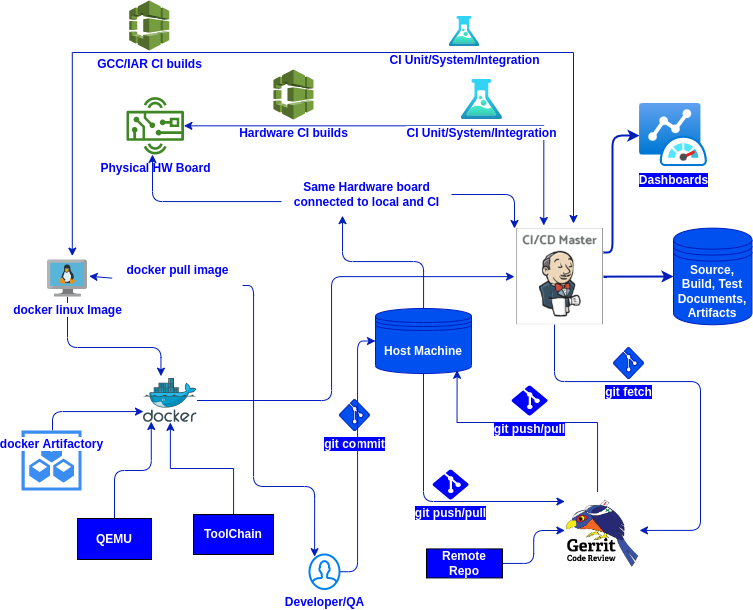
\includegraphics{CI_Infrastrcuture_2}}
\caption{Embedded CI/CD Workflow}\label{fig:CI_Infrastrcuture_2} \end{figure}

\subsection*{Using Docker for Environment Consistency and QEMU:} To maintain a
consistent development environment, Docker~\cite{anderson2015docker} containers
are utilized to package necessary dependencies for the Zephyr RTOS firmware
compilation, reducing discrepancies during builds. QEMU~\cite{bellard2005qemu},
as a hardware emulator, enables testing in a simulated environment, which is
crucial for early detection of potential issues.

The Docker image~\cite{bui2015analysis} with QEMU is then stored in the JFrog
Artifactory~\cite{Artifact8:online} for use by developers.

\subsection*{Compilation Builds with GCC and IAR:} Different compiler
configurations are essential to cater to varied needs.
GCC~\cite{GCCtheGN9:online}, known for its practicality, offers a suite of compilers for different
programming languages. Conversely, IAR~\cite{AboutIAR98:online} provides
specialized compilers for embedded systems, aiming for optimal performance and
smaller footprints, which are vital for resource-constrained devices. Both
compilers ensure the Zephyr RTOS firmware is compatible across diverse platforms.

Automated processes compile the code post-modification, utilizing tools such as
Clang Static Analyzer~\cite{kremenek2008finding} and
Coverity~\cite{imtiaz2019developers} for static analysis to identify potential
issues.

\subsection*{Testing Frameworks:}

Ztest~\cite{TestFram11:online}, also known as the Zephyr Test Framework,
is a unit testing framework~\cite{runeson2006survey}
designed to validate the correctness of individual segments of Zephyr RTOS
code~\cite{TestFram11:online}.

The Pytest framework~\cite{hunt2019pytest}, on the other hand, examines the
overall functionality and interactions between the system's components, serving
as a tool for system and integration testing~\cite{TheFourL21:online}.

\textbf{Deployment and Continuous Monitoring:}

Jenkins~\cite{jenkins1963jenkins}, a renowned continuous integration tool~\cite{smart2011jenkins}, manages
various essential operations within the development
workflow~\cite{sayfan2017mastering}. Each code submission to the repository~\cite{milanesio2013learning}
initiates a series of processes including code compilation, unit testing~\cite{runeson2006survey} with
Ztest framework~\cite{TestFram11:online}, and system and integration
testing~\cite{TheFourL21:online} via the Pytest framework~\cite{hunt2019pytest}.
Developers are promptly informed of any issues detected during the build or test
stages.

The Jenkins interface offers detailed dashboards showcasing metrics like
instances of build failure and processing times. Moreover, extensive reports are
archived for future analysis. Continuous monitoring post-deployment is vital to
ensure the firmware's steady and efficient functioning~\cite{mcallister2015mastering}.
\pagebreak

\subsection{Simplified Current Workflow}

The Figure:~\ref{fig:simplified_workflow_current} illustrates further simplified depiction of the
current workflow~\ref{fig:CI_Infrastrcuture_2} used in the case company.

% \begin{figure}[H]
%         \centering
%         \adjustbox{width=\textwidth}{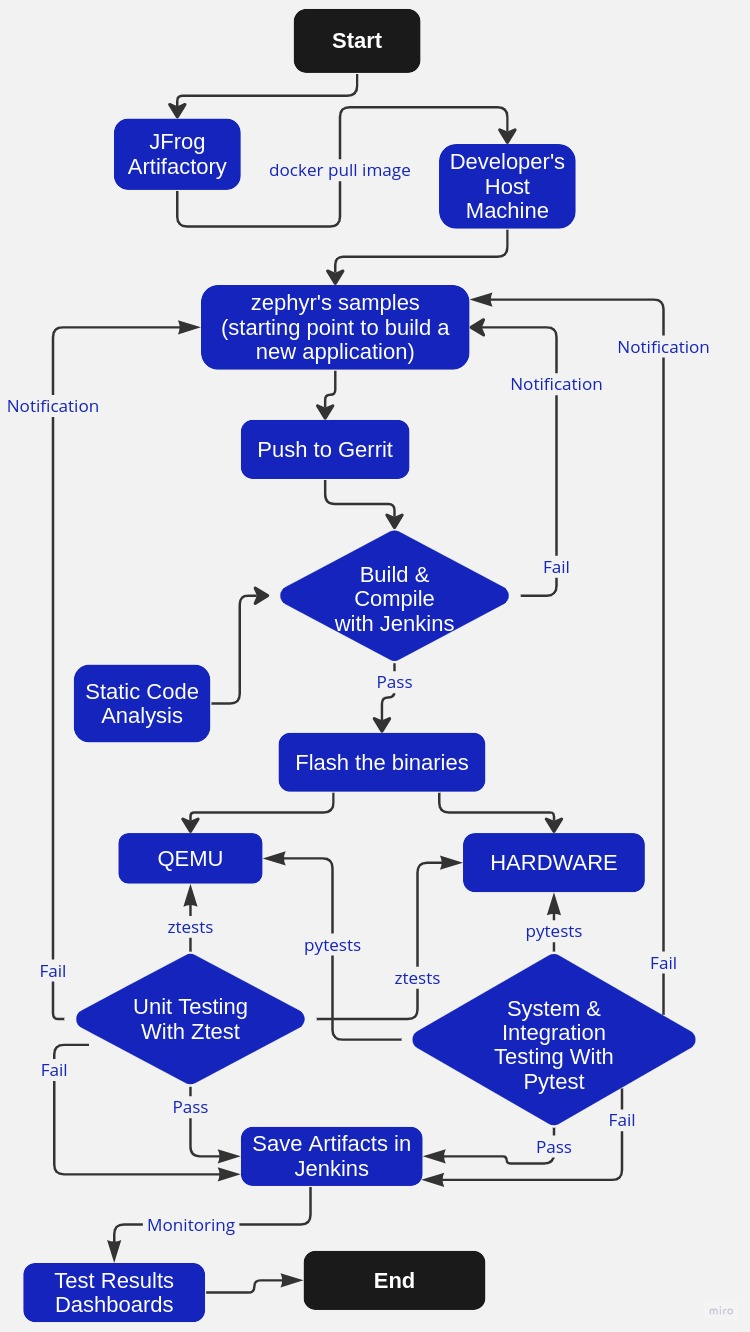
\includegraphics{simplified_workflow_current}}
%         \caption{Simplified Current Workflow}\label{fig:simplified_workflow_current}
% \end{figure}
% \begin{figure}[H]
%         \centering
%         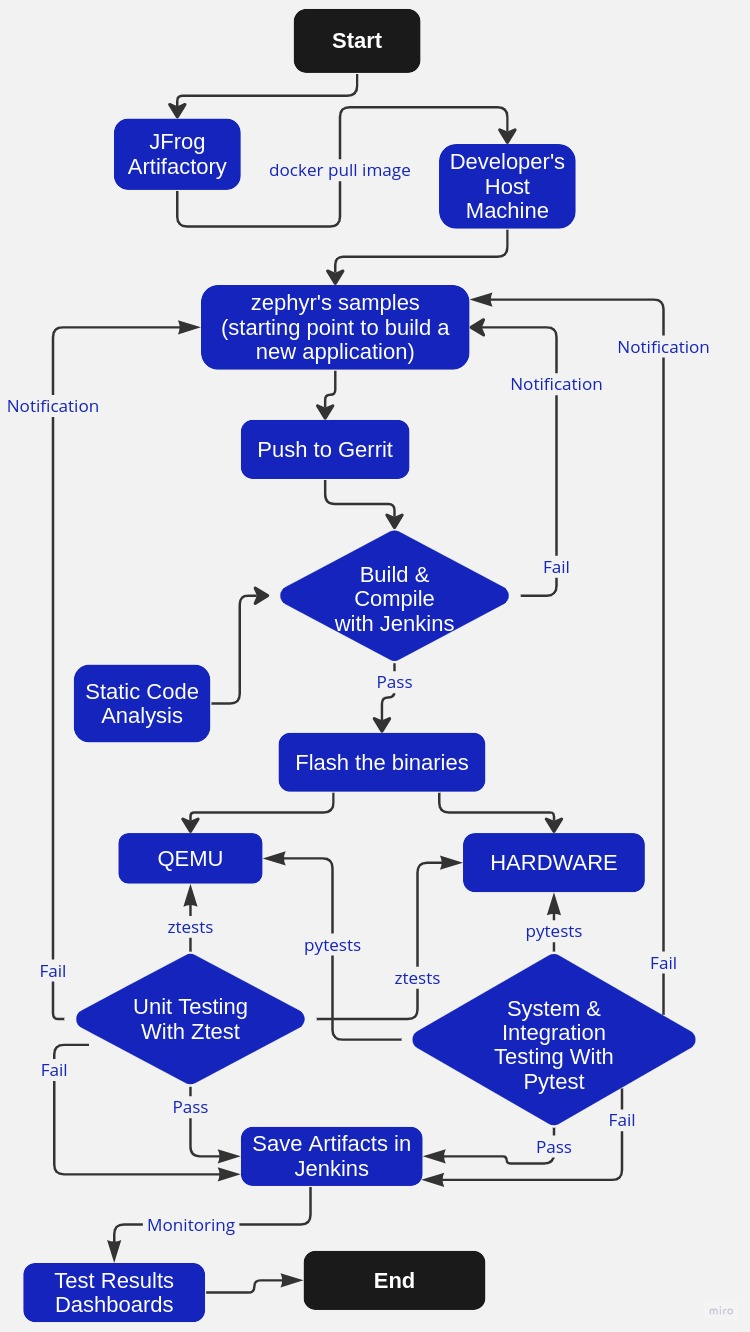
\includegraphics[width=\textwidth]{simplified_workflow_current}
%         \caption{Simplified Current Workflow}
%         \label{fig:simplified_workflow_current}
%     \end{figure}

\begin{figure}[H]
\centering
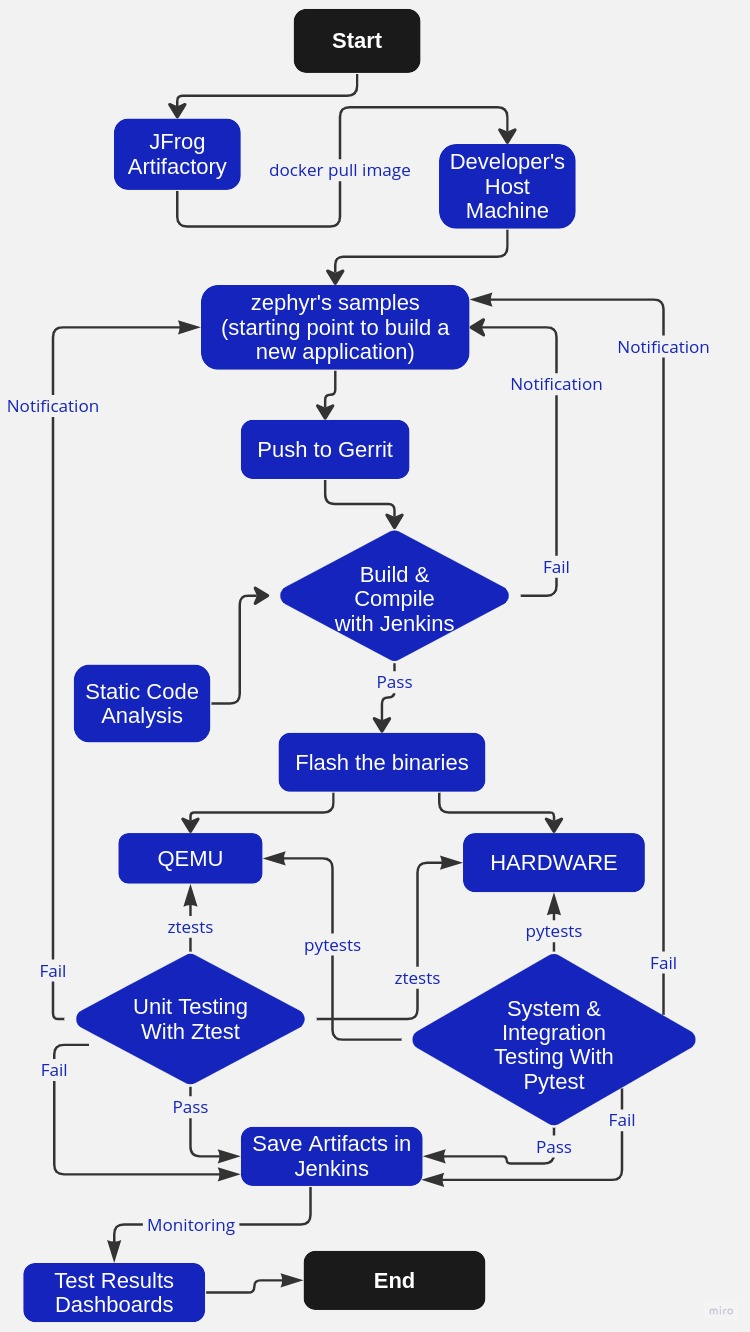
\includegraphics[width=\textwidth,height=0.8\textheight,keepaspectratio]{simplified_workflow_current}
\caption{Simplified Current Workflow}
\label{fig:simplified_workflow_current}
\end{figure}

\section{Proposed Workflow With Fuzzing}
In light of the previously detailed current analysis, it becomes imperative to
explore enhancements that could further fortify the software development
lifecycle. One such augmentation revolves around the incorporation of
fuzzing, thereby aiming to unearth vulnerabilities
that conventional testing approaches might overlook.

The Figure:~\ref{fig:simplified_workflow_proposed} illustrates a simplified depiction of the
proposed workflow used in the case company.
\begin{figure}[H]
\centering
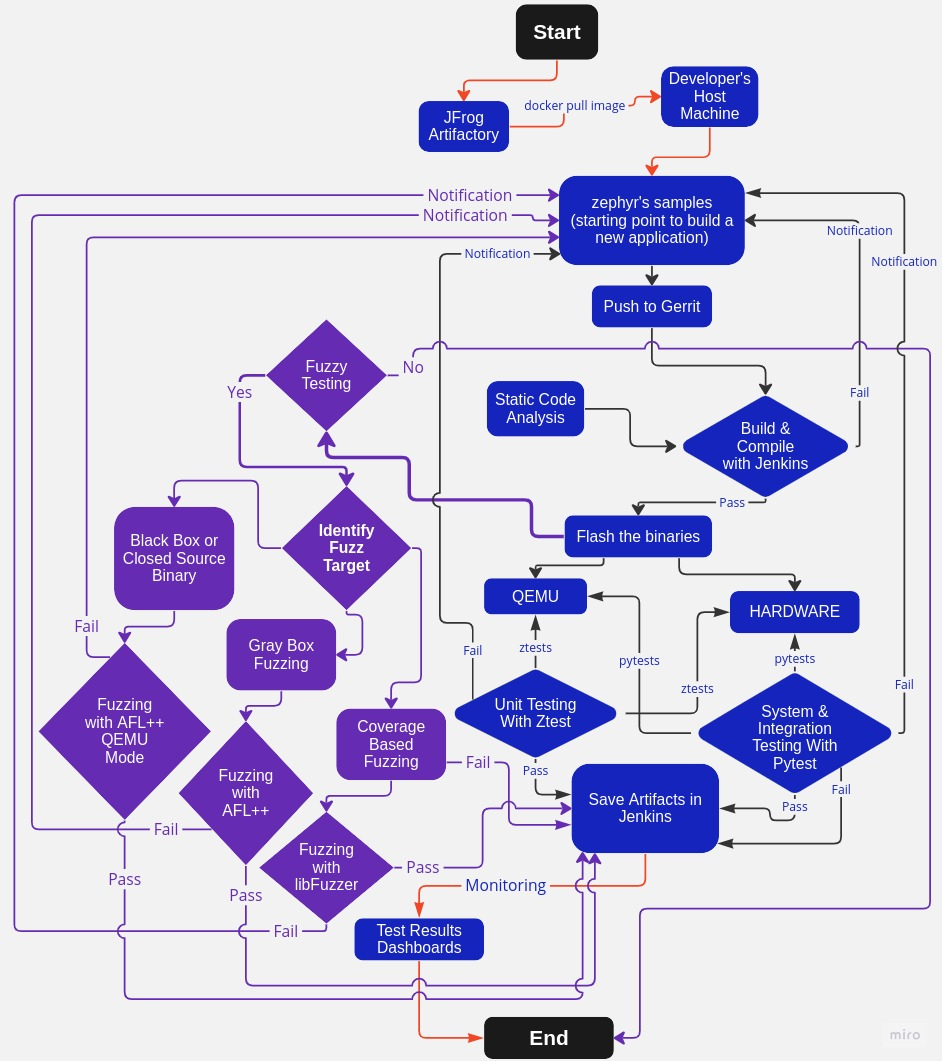
\includegraphics[width=\textwidth,height=0.8\textheight,keepaspectratio]{fuzzy_current_proposed}
%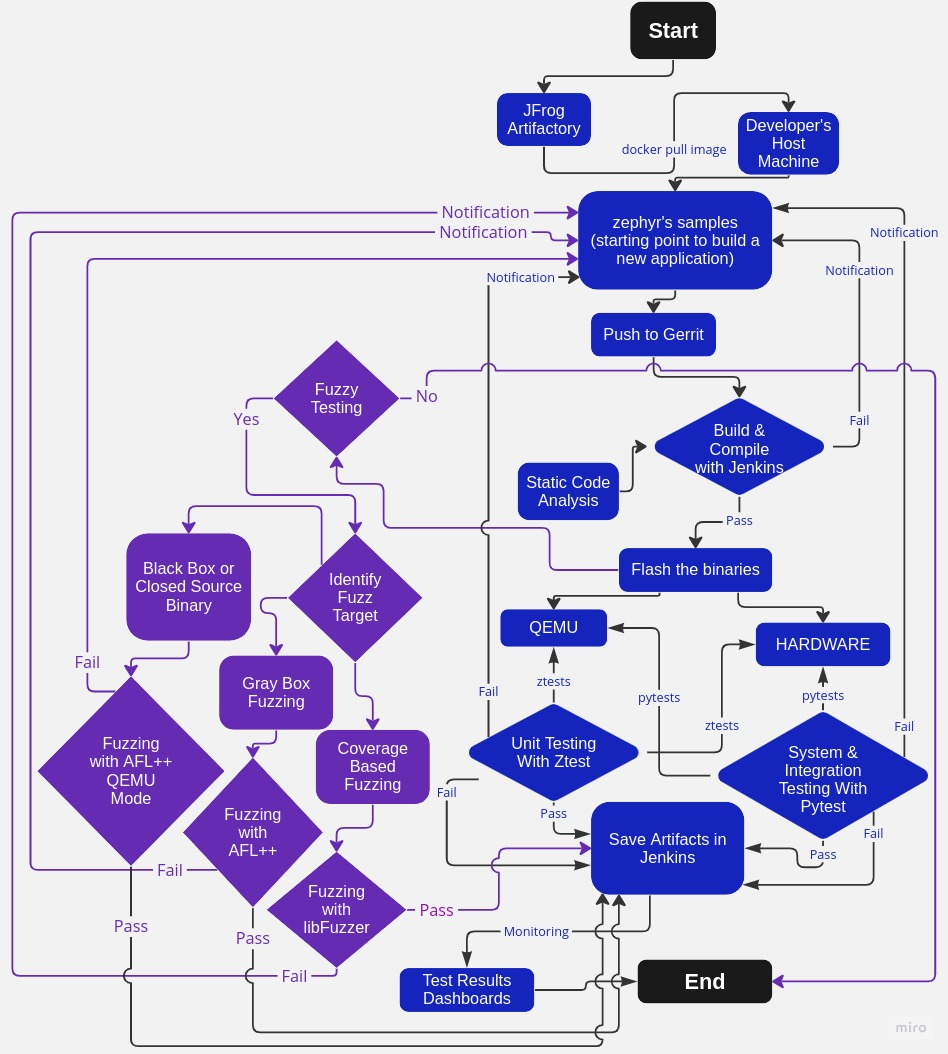
\includegraphics[width=\textwidth,height=0.8\textheight,keepaspectratio]{simplified_workflow_proposed}
\caption{Simplified Proposed Workflow}
\label{fig:simplified_workflow_proposed}
\end{figure}

\subsection*{Integration of Fuzzing}

Post the flashing of the firmware image~\cite{Firmware14:online}, an assessment
is undertaken to evaluate the compatibility of the binaries with fuzz testing, a process known as
``identifying the target'' in fuzz testing terminology and called as \gls{fuzz_target}.
This step is crucial for selecting the correct fuzz testing methodology.

Based on the characteristics of the \gls{fuzz_target}, various fuzz testing
methods are applicable. When the binary's compiler is identified, gray box
fuzzing~\cite{jamil2016software}, which strikes a balance between
blackbox'~\cite{godefroid2007random}~\cite{jamil2016software} and
whitebox'~\cite{godefroid2007random}~\cite{jamil2016software} fuzzing, should be
employed using afl-fuzz++~\cite{257204}. This approach encompasses
coverage-guided fuzzing~\cite{abran2001guide}, performed with
libfuzzer\cite{libFuzze17:online}. In contrast, if the binary's compiler is
unidentified, which is common with
black-box~\cite{jamil2016software}~\cite{pudas2017improving} or closed-source
binaries, the utilization of afl-fuzz in conjunction with QEMU is
advised~\cite{AFLplusp57:online}.

The enhanced workflow adds a supplementary layer of security
by methodically evaluating the software with a spectrum of unconventional
inputs. This process aids in pinpointing and mitigating potential
vulnerabilities before the software is deployed.

\begin{longtable}{p{1cm}p{3.7cm}p{3.7cm}p{3.7cm}}
\caption{Comparison of Current and Proposed System Workflows with Fuzzy Testing}
\label{tab:system_workflows_comparison_fuzzy} \\
\toprule
\textbf{Step} & \textbf{Current Workflow} & \textbf{Proposed Workflow} & \textbf{Changes and Notes} \\
\midrule
\endfirsthead

\toprule
\textbf{Step} & \textbf{Current Workflow} & \textbf{Proposed Workflow} & \textbf{Changes and Notes} \\
\midrule
\endhead

1 & Retrieve Docker Image from JFrog Artifactory & Retrieve Docker Image from JFrog Artifactory & No changes required \\
\midrule
2 & Develop sample application in Zephyr & Develop sample application in Zephyr & No changes required \\
\midrule
3 & Push to Gerrit for version control & Push to Gerrit for version control & No changes required \\
\midrule
4 & Compilation and building with Jenkins & Compilation and building with Jenkins & No changes required \\
\midrule
5 & Static code analysis with Jenkins & Static code analysis with Jenkins & No changes required \\
\midrule
6 & Flash binary images for both QEMU and hardware & Check eligibility for fuzz testing of the flashed binaries & Addition of a new step to determine eligibility for fuzz testing \\
\midrule
7 & Perform unit testing with ztest & Identify fuzz target based on eligibility & Addition of a new step for identifying the fuzz target \\
\midrule
8 & Conduct system and integration testing with pytest & Select appropriate fuzzing tools like AFL++, libFuzzer based on the target & Addition of a new step for selecting the appropriate fuzzing tool \\
\midrule
9 & Notification of failures & Validate the presence of bugs or vulnerabilities during unit, system, or fuzz testing & Addition of notifications for vulnerabilities identified during fuzz testing \\
\midrule
10 & Save test results in Artifactory & Record fuzz testing results & Addition of a new step to save the results of fuzz testing \\
\midrule
11 & Monitor test results & Monitor test results, including pass and fail ratios & Addition of monitoring for results of fuzz testing \\
\bottomrule
\end{longtable}


\subsection*{Benefits and Challenges:}
\textbf{Benefits:}~\cite{liang2018fuzz}~\cite{klees2018evaluating} \\
\begin{itemize}
    \item Enhances software security by proactively identifying and addressing vulnerabilities, thereby reducing risks associated with software exploits.
    \item Fosters the development of more resilient software, as developers become aware of potential issues and enhance their coding practices\cite{HowCICDI34:online}.
\end{itemize}

\textbf{Challenges:}~\cite{liang2018fuzz}~\cite{klees2018evaluating} \\
\begin{itemize}
    \item Resource-intensive, potentially extending the duration of the CI/CD pipeline.
    \item May yield false positives, necessitating additional time and resources to identify genuine vulnerabilities.
    \item Determining the appropriate times for conducting fuzz testing, such as off-peak hours or weekends.
    \item Establishing the optimal duration for fuzz testing.
    \item Managing test results, including logging failure conditions and steps to reproduce the issue~\cite{FuzzingC40:online}.
\end{itemize}


\clearpage
% Theoretical background
%\clearpage%if the chapter heading starts close to bottom of the page, force a
% line break and remove the vertical vspace
\vspace{21.5pt}
\chapter{Design, Implementations and Results}

This chapter details the methodology adopted for incorporating fuzzing into
sample targets known as \gls{fuzz_target} operating on the Zephyr Real-Time Operating System
(RTOS)~\cite{Security75:online}. These targets were selected to demonstrate the
practical applicability of the research.

Various fuzzers have been discussed in preceding sections, but
AFL++~\cite{257204} and libFuzzer~\cite{libFuzze17:online} were selected for
demonstration because of their unique capabilities and widespread adoption.
These fuzzers underline the importance of the study, considering the widespread
use of real-time operating systems in contemporary embedded devices.

In addition to the \acrlong{poc} usage of AFL++~\cite{257204}, and libFuzzer~\cite{libFuzze17:online}, the
AFL++ in QEMU mode~\cite{AFLplusp57:online} was utilized to broaden the scope of
the study, enabling fuzz testing of closed-source binaries~\cite{nagy2021breaking} within the company's case.
This inclusion demonstrates the adaptability of the fuzzing methodology and its
practical applicability to a range of software types.

For the execution of fuzzing tests, a Linux environment was utilized, where
AFL++~\cite{257204}, AFL++ in QEMU mode~\cite{AFLplusp57:online} are used with Docker~\cite{anderson2015docker}~\cite{aflplusp99:online},
and libFuzzer\cite{libFuzze17:online} were pre-installed, and the Zephyr RTOS~\cite{Security75:online}
environment was configured.


\section{Implementations Using AFL++}
This section delineates the detailed steps for setting up the
AFL++~\cite{257204} fuzzer using a Docker~\cite{anderson2015docker}~\cite{aflplusp99:online}
container and compiling the target program.

The selection of the AFL++ Docker image~\cite{aflplusp99:online} as the basis for the initial setup was
driven by the recommendations provided by the AFL++ documentation~\cite{GitHubAF78:online}. This particular
image is endorsed due to its comprehensive inclusion of all necessary AFL++ tools,
consolidated in a singular location, thereby facilitating a streamlined
and efficient setup process~\cite{257204}.

Steps to start fuzzing with AFL++:

\subsection*{Step 1: Docker Script for AFL++}
\label{subsec:docker script for afl-fuzz}
The first step involves pulling the AFL++ Docker image and running a container:
\begin{minted}[linenos,frame=lines,baselinestretch=1.2,breaklines]{sh}
#!/bin/bash
# Pull the AFL++ Docker image
$ docker pull aflplusplus/aflplusplus
# Run a container using the pulled image
$ docker run -ti -v /home/uname:/home/uname --name afl_container aflplusplus/aflplusplus
# Get into the container
$ docker exec -it afl_container /bin/bash
\end{minted}

This script facilitates the deployment of the AFL++ fuzzer in a Docker container,
streamlining the setup process for fuzzing tests.

\subsection*{Step 2: List of Files}
The relevant files for the next step are:
\begin{itemize}
    \item \texttt{main.c}: The target program in Appendix:~\ref{appx:first}.
    \item \texttt{CMakeLists.txt}: Build configuration file.
\end{itemize}

The detailed implementation of the target program can be
found in Appendix:~\ref{appx:first}. This program, written
in C, exemplifies the integration of fuzz testing for a sample application.

\subsection*{Explanation of the Main Program:}
The \texttt{main.c} program serves as the target for the fuzz testing,
designed to illustrate potential vulnerabilities.
It's structured to simulate a scenario where specific inputs could trigger a
failure case, providing a practical example for the fuzzing tests conducted.

This particular program was selected due to its specific characteristics
essential for fuzz testing. Fuzz testing is coverage-based and requires hiding a
failure point— in this case, a write through a null pointer~\cite{spoto2011precise}—deep within the call
structure of the program. Such concealed failures can be challenging to reveal
with randomly-selected input, yet a fuzzer aims to uncover them in a relatively
linear time by systematically exploring each function~\cite{FuzzingE54:online}.

Even in situations where the probability of discovering the failure is low,
such as \(1 \times 2^{56}\), which typically requires significant computational
time and resources, the fuzzer can detect the vulnerability in considerable time.

The program contains several key components:

\begin{itemize}
\item \textbf{global\_null\_ptr}: A pointer that, under certain conditions,
can be triggered to write through a null, simulating a failure.
\item \textbf{key Array and found Array}: These arrays are used to check against
the input data, and keep track of discovered keys.
\item \textbf{GEN\_CHECK Macro}: This macro generates a series of check
functions that recursively call each other to simulate a deep call tree.
\end{itemize}

Upon execution, the program reads input data from a file. It then processes
this data through the series of check functions generated by
the \texttt{GEN\_CHECK} macro. If a match with the key array is found,
it simulates a failure by attempting a write through the \texttt{global\_null\_ptr}.
The failure case is hidden deep within the call tree, making it difficult to
discover through the random inputs but still discoverable through fuzz testing.

For a more detailed view of the \texttt{main.c} file, refer to
Appendix~\ref{appx:first}.

\textbf{Explanation of the CMakeLists.txt:}
The \texttt{CMakeLists.txt} file is used for configuring the build system
of the \texttt{sample\_zephyr\_afl} project in the zephyr RTOS. Here is an
explanation of its components:

\begin{itemize}
    \item \texttt{cmake\_minimum\_required(VERSION 3.20.0)}: This command
    specifies the minimum version of CMake that is required, which is version
    3.20.0 in this case.
    \item \texttt{project(sample\_zephyr\_afl)}: This command sets the name
    of the project to \texttt{sample\_zephyr\_afl}.
    \item \texttt{option(USE\_AFL "Use afl" OFF)}: This command declares an
    option named \texttt{USE\_AFL} that determines whether to use AFL. It is
    set to \texttt{OFF} by default.
    \item The conditional block \texttt{if(USE\_AFL)} checks
    whether \texttt{USE\_AFL} is turned on. If it is, the compiler is
    set to \texttt{afl-gcc-fast}~\cite{AFLplusp13:online}, and additional
    compiler flags for coverage are added. If \texttt{USE\_AFL} is turned off,
    the compiler is set to \texttt{gcc}~\cite{GCCtheGN9:online}.
    \item \texttt{add\_executable(zephyr\_aflfuzzer src/main.c)}: This
    command specifies that an executable named \texttt{zephyr\_aflfuzzer}
    should be created from the source file \texttt{src/main.c}.
\end{itemize}

For a more detailed view of the \texttt{CMakeLists.txt} file, refer to
Appendix:~\ref{appx:first}.

\subsection*{Step 3: Build and Compile}
A new directory, \texttt{build}, is created to contain all the build files.
The \texttt{cmake} command is invoked with the \texttt{-DUSE\_AFL=ON} option,
indicating that the build should be configured to
use \texttt{afl-gcc-fast}~\cite{AFLplusp13:online}.

\begin{minted}[linenos,frame=lines,baselinestretch=1.2,breaklines]{sh}
    $ mkdir build
    $ cd build
    $ cmake -DUSE_AFL=ON ..
    $ make
\end{minted}

\subsection*{Step 4: Valid Input for the Target}
A binary file is created with a specific sequence of bytes.
This file will serve as the initial and valid input or corpus for the fuzzer,
allowing it to explore different code paths.

\begin{minted}{sh}
    $ echo -n -e '\x9e\x21\x0c\x18\x9d\xd1\x7e' > input_data/test_data.bin
\end{minted}

\subsection*{Step 5: Fuzz Testing with AFL++}
AFL++ is invoked with the \texttt{afl\-fuzz} command inside the docker container,
specifying the input directory containing the corpus \texttt{input\_data} and
the output directory \texttt{output}. The built binary \texttt{zephyr\_aflfuzzer}
is then executed with AFL++'s syntax for specifying input files.


\begin{minted}{sh}
    $ afl-fuzz -i input_data/ -o output/ -- ./sample_zephyr_afl/build/zephyr_aflfuzzer @@
\end{minted}

This section breaks down the components of this command~\cite{257204}:

\begin{itemize}
    \item \texttt{afl-fuzz}: This is the command to initiate the AFL++ fuzzer.
    \item \texttt{-i input\_data/}: The \texttt{-i} flag specifies the
    input directory containing the `corpus' of sample input files,
    which serve as a basis to generate new test cases.
    \item \texttt{-o output/}: The \texttt{-o} flag denotes the output
    directory where AFL stores the results of the fuzzing session,
    including any crashes or hangs it discovers.
    \item \texttt{--}: This symbol denotes the end of the options passed
    to the AFL fuzzer. Any parameter listed after this is considered as
    an argument to the program being fuzzed, not as an option to AFL.
    \item \texttt{./sample\_zephyr\_afl/build/zephyr\_aflfuzzer}: This is the
    path to the target binary that will be fuzzed by AFL.
    \item \texttt{@@}: This placeholder is replaced by AFL with the name of a
    file containing the test case each time the target binary is run,
    allowing AFL to run the program with a multitude of different inputs
    without needing to modify the command line each time.
\end{itemize}
\subsection*{Step 6: Results, Analysis and Report}~\label{subsec:execution afl-fuzz}
The Figure:~\ref{fig:afl_execute_1} shows the AFL++ execution screen.
\begin{figure}[H]
        \adjustbox{width=\textwidth}{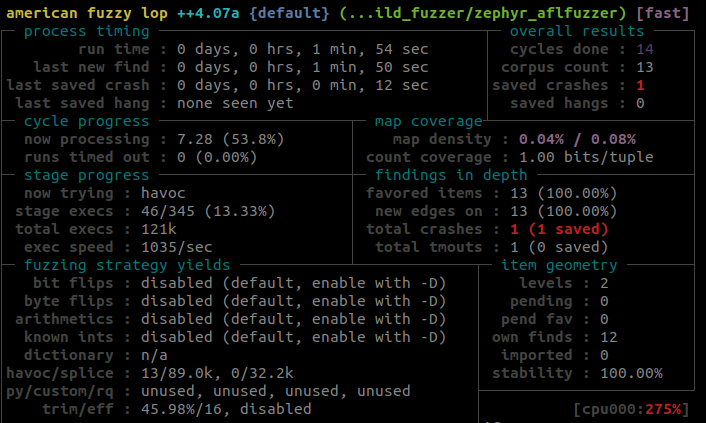
\includegraphics{afl_execute_1}}
        \caption{AFL++ Execution Screen}~\label{fig:afl_execute_1}
\end{figure}

Important elements of the user interface shown below~\cite{257204}:

\begin{itemize}
    \item \textbf{process\_timing:} This section shows how long the fuzzer has
    been running and the current time.
    \item \textbf{stage progress:} Here, AFL++ displays the progress of the
    current fuzzing stage in terms of execution and the total number of inputs
    to be tested in this stage.
    \item \textbf{findings in depth:} This area provides details about the paths
    discovered, including the number of unique crashes, hangs, and paths found
    during the fuzzing session.
    % \item \textbf{fuzzing strategy yields:} This section gives insights into the
    % effectiveness of various fuzzing strategies by showing how many new paths, crashes, or hangs each strategy has yielded.
    \item \textbf{item geometry:} This displays information related to the paths
    taken through the program, such as the depth and width of the explored paths.
    %\item \textbf{pending favs:} It shows the number of favored paths (interesting inputs) that are yet to be processed.
    %\item \textbf{map coverage:} This section gives a snapshot of the code coverage, indicating the percentage of the target's codebase that has been executed by the inputs generated so far.
    %\item \textbf{speed:} This denotes the execution speed of the fuzzer, typically represented in executions per second.
    %\item \textbf{cycle progress:} This shows the progress of the current fuzzing cycle, indicating how much of the input corpus has been processed in this cycle.
    %\item \textbf{total execs:} This is a count of the total number of input cases that AFL++ has executed since the start of the fuzzing session.
    %\item \textbf{exec reliability:} This metric shows the reliability of the execution, highlighting if any executions were aborted.
    %\item \textbf{exec stability:} This indicates the stability of the target program during fuzzing, represented as a percentage.
    %\item \textbf{has\_new\_finds:} This field will be highlighted if AFL++ has found new, unique crashes or paths since the last UI update.
    %\item \textbf{has\_uniq\_finds:} This will be highlighted if AFL++ has found any new unique crashes, hangs, or paths since the last UI update.
    %\item \textbf{command:} At the bottom of the screen, the exact command-line used to start AFL++ is displayed.
\end{itemize}

As depicted in Figure:~\ref{fig:afl_execute_1}, the binary generated
(as detailed in Appendix~\ref{appx:first}) resulted in AFL++ creating a total of
13 corpus and identifying one crash. Remarkably, a scenario with a
probability of \(1\) in \(2^{56}\), which would traditionally
require several months to years of computation in a large datacenter,
was resolved by the fuzzer in under two minutes~\cite{FuzzingE54:online}.

The resulting outputs are stored in the \textit{output} directory.
The coverage report of the execution can be generated using \textit{afl-cov}~\cite{GitHubmr91:online}.
The corresponding command is as follows:

\begin{minted}{sh}
    $ afl-cov -d output/ --coverage-cmd "./sample_zephyr_afl/build/zephyr_aflfuzzer @@" --code-dir ./sample_zephyr_afl/
\end{minted}

The Figure~\ref{fig:afl_cov} shows the \texttt{afl-cov} report of the execution.
\begin{figure}[H]
        \adjustbox{width=\textwidth}{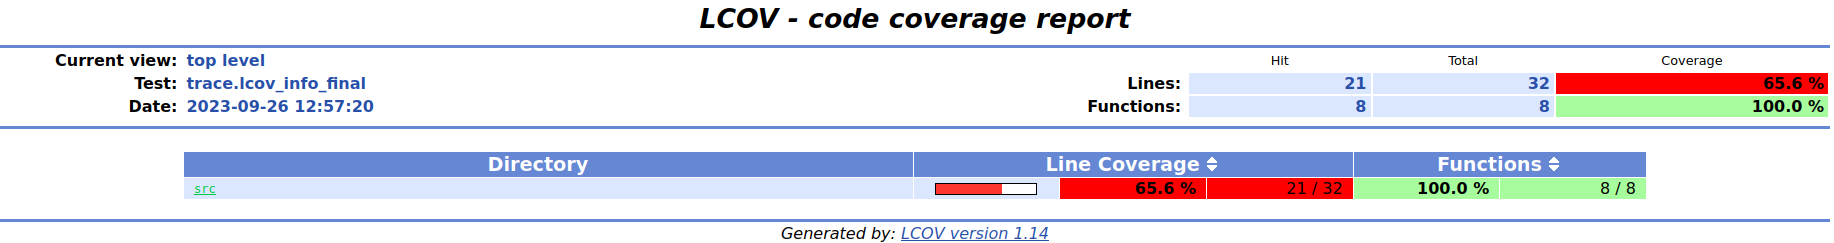
\includegraphics{afl_cov}}
        \caption{LCOV Coverage Report~\cite{UbuntuMa97:online}}\label{fig:afl_cov}
\end{figure}

AFL++ includes a visualization tool called \texttt{afl-plot}~\cite{AFLFunct92:online},
which is instrumental in assessing the performance of fuzzing campaigns.
This tool generates a series of graphs that provide insights into several
crucial metrics throughout the fuzzing process. These metrics include,
but are not limited to, the number of crashes discovered,
the speed of execution, and the progression of path discovery over time.

\begin{minted}{sh}
    $ afl-plot output/default/ output/output_plot/
\end{minted}

The Figure:~\ref{fig:afl_plot} shows the \texttt{afl-plot} report of the execution.
\begin{figure}[H]
        \adjustbox{width=\textwidth}{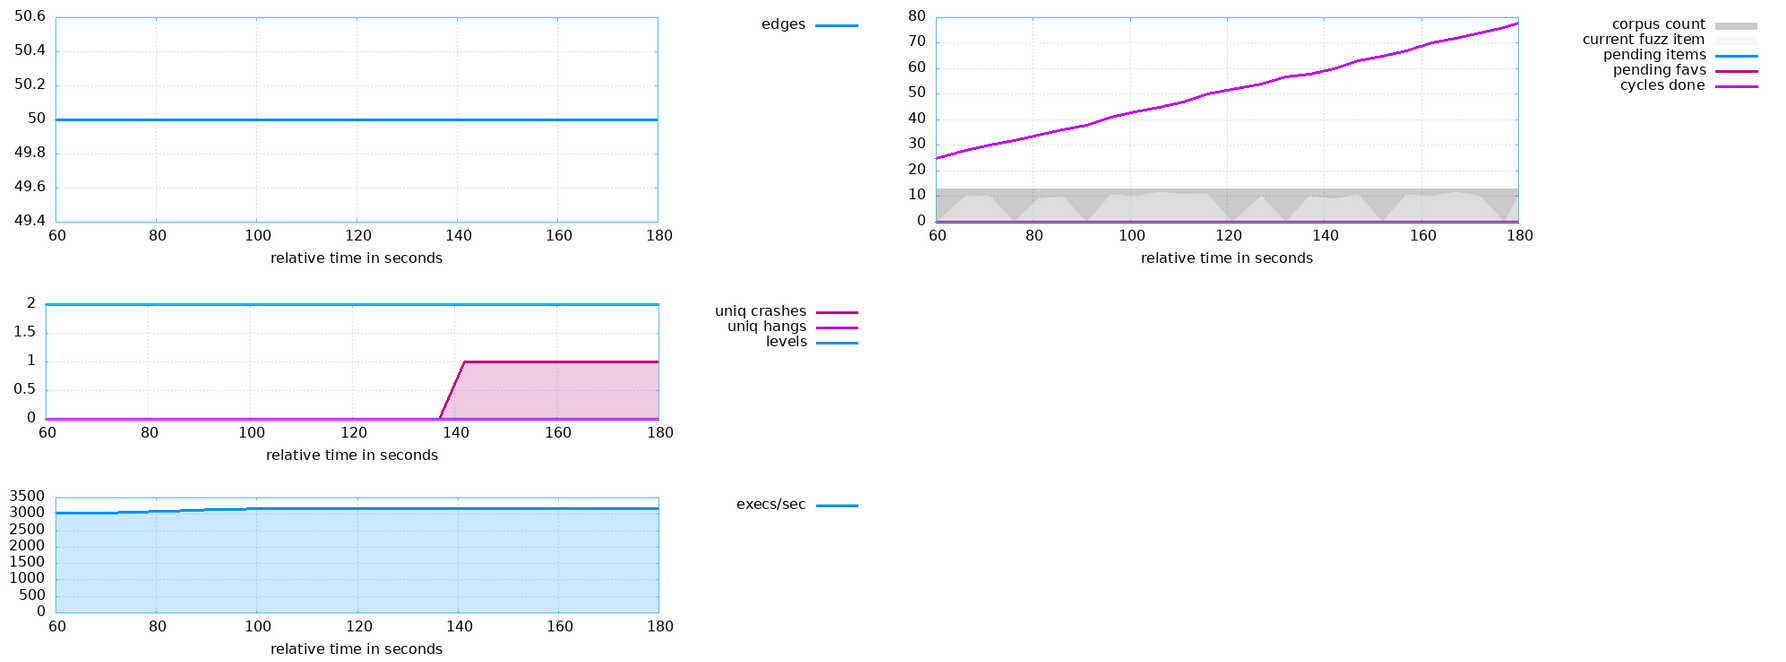
\includegraphics{afl_plot}}
        \caption{\texttt{afl-plot} Report}~\label{fig:afl_plot}
\end{figure}

The fuzzing tests effectively utilize the AFL++ fuzzer, along with tools such as
``afl-cov''~\cite{GitHubmr91:online} and ``afl-plot''~\cite{AFLFunct92:online}.
These tools highlight vulnerabilities while also providing comprehensive
coverage reports and graphical representations of the test data. The AFL++
fuzzer is notable for its ability to quickly identify vulnerabilities, even
those deeply embedded within the code structure. This process is enhanced by
``afl-cov'' and ``afl-plot'', which offer detailed insights into the system's
susceptibility to potential threats. The findings of this study reveal the
significant advantages of incorporating AFL++ into the development cycle,
emphasizing its potential to fortify system security.

\section{Implementations Using libFuzzer}
LibFuzzer~\cite{libFuzze17:online}, an integral part of the LLVM Compiler~\cite{libFuzze42:online} Infrastructure,
is chosen for this \acrlong{poc} due to its distinct attributes and capabilities.
LibFuzzer is renowned for its efficiency in performing coverage-guided fuzzing,
which is instrumental in identifying hidden vulnerabilities within a system~\cite{fuzzingt51:online}.

The fuzzer's seamless integration with the Clang compiler~\cite{ClangCLa81:online} and its capability
to perform in-memory fuzzing make it a valuable tool in assessing the security
and robustness of software systems.

Steps to start fuzzing with libFuzzer:

\subsection*{Step 1: Setting up Environment}
To set up the necessary environment, a Linux-based operating system,
specifically Ubuntu, is utilized. Furthermore, the installation of a recent
version of the Clang compiler is requisite for the successful execution of the
libFuzzer~\cite{ClangCLa81:online}.

\subsection*{Step 2: List of Files}
The relevant files for the next step are:
\begin{itemize}
    \item \texttt{main.c}: The target program in Appendix:~\ref{appx:second}.
    \item \texttt{CMakeLists.txt}: Build configuration file.
\end{itemize}

The detailed implementation of the target program can be
found in Appendix:~\ref{appx:second}.

Comparing this program in Appendix:~\ref{appx:second} to the one utilized for
AFL++ in Appendix:~\ref{appx:first}, there are fundamental differences that
can be highlighted:


\begin{itemize}
    \item \textbf{Entry Point:} In the context of libFuzzer, the program uses a function
    named \texttt{LLVMFuzzerTestOneInput} as the entry point,
    which is specifically designed for integration with libFuzzer.
    This contrasts with the AFL++ target program, where the
    \texttt{main} function serves as the entry point.
    \item \textbf{Input Handling:} The libFuzzer target program directly uses
    the input data provided to the \texttt{LLVMFuzzerTestOneInput} function,
    representing a more straightforward handling of input compared to the
    AFL++ target program, which might necessitate additional steps for input
    retrieval and processing.
\end{itemize}

\textbf{Explanation of the CMakeLists.txt:}
The \texttt{CMakeLists.txt} file is used for configuring the build system
of the \texttt{sample\_zephyr\_libFuzzer} project in the zephyr RTOS.
Here is an explanation of its components:

\begin{itemize}
    \item \texttt{cmake\_minimum\_required(VERSION 3.20.0)}: Specifies the minimum required version of CMake to be 3.20.0.

    \item \texttt{project(sample\_zephyr\_libfuzzer)}: Names the project as \texttt{sample\_zephyr\_libfuzzer}.

    \item \texttt{option(USE\_LIBFUZZER "Build with libfuzzer" OFF)}: Declares an option \texttt{USE\_LIBFUZZER}, which is turned OFF by default but can be set to ON to enable building with libFuzzer.

    \item \texttt{set(CMAKE\_C\_COMPILER clang)}: Sets the C compiler for the project to Clang.

    \item \texttt{if(USE\_LIBFUZZER)}: Checks if \texttt{USE\_LIBFUZZER} is enabled.

    \begin{itemize}
        \item \texttt{add\_definitions(-DUSE\_LIBFUZZER)}: Adds a definition for \texttt{USE\_LIBFUZZER} for the preprocessor.

        \item \texttt{set(CMAKE\_C\_FLAGS "... -fsanitize=fuzzer,address,undefined")}: Sets the compiler flags to enable sanitizers and fuzzer.

        \item \texttt{set(CMAKE\_EXE\_LINKER\_FLAGS "... -fsanitize=fuzzer,address,undefined")}: Sets the linker flags to enable sanitizers and fuzzer.

        \item \texttt{set(CMAKE\_C\_FLAGS "... -fprofile-instr-generate -fcoverage-mapping")}: Enables flags for generating profile instrumentation and coverage mapping.
    \end{itemize}

    \item \texttt{add\_executable(zephyr\_libfuzzer src/main.c)}: Defines an executable target named \texttt{zephyr\_libfuzzer} from the source file \texttt{src/main.c}.

    \item \texttt{if(USE\_LIBFUZZER)}: If \texttt{USE\_LIBFUZZER} is enabled, sets additional linker flags for the target \texttt{zephyr\_libfuzzer} to enable the necessary sanitizers for fuzzing.
\end{itemize}

\subsection*{Step 3: Build and Compile}
A new directory, \texttt{build}, is created to contain all the build files.
The \texttt{cmake} command is invoked with the \texttt{-DUSE\_LIBFUZZER=ON} option,
indicating that the build should be configured to
use \texttt{clang}~\cite{ClangCLa81:online} with libFuzzer.

\begin{minted}[linenos,frame=lines,baselinestretch=1.2,breaklines]{sh}
    $ mkdir build
    $ cd build_fuzzer
    $ cmake -DUSE_LIBFUZZER=ON ..
    $ make
    $ ./zephyr_libfuzzer
\end{minted}

\subsection*{Step 4: Testing, Results and Analysis}
The `CMake' configuration for the \texttt{sample\_zephyr\_libfuzzer} project
provides a solid foundation for enabling fuzz testing with \texttt{libFuzzer}
and Clang's sanitizers~\cite{GitHubgo55:online}. The option to toggle the
\texttt{libFuzzer} integration is valuable, allowing the program to be compiled
with or without the fuzzing infrastructure. When the \texttt{USE\_LIBFUZZER}
option is activated, the system properly applies the necessary compiler and
linker flags to include \texttt{libFuzzer},
address sanitizer~\cite{GitHubgo55:online}, and
undefined behavior sanitizer~\cite{GitHubgo55:online}. Additionally,
the inclusion of instrumentation flags for profile generation and coverage
mapping indicates a commitment to not only identifying vulnerabilities but also
to measuring the coverage of the testing process. This dual focus on
vulnerability discovery and code execution coverage provides comprehensive
insight into the program's resilience against arbitrary and malicious inputs,
ultimately offering a valuable report on its security status.


The Figure:~\ref{fig:lib_fuzzer} shows the libFuzzer execution output.
\begin{figure}[H]
    \adjustbox{width=\textwidth}{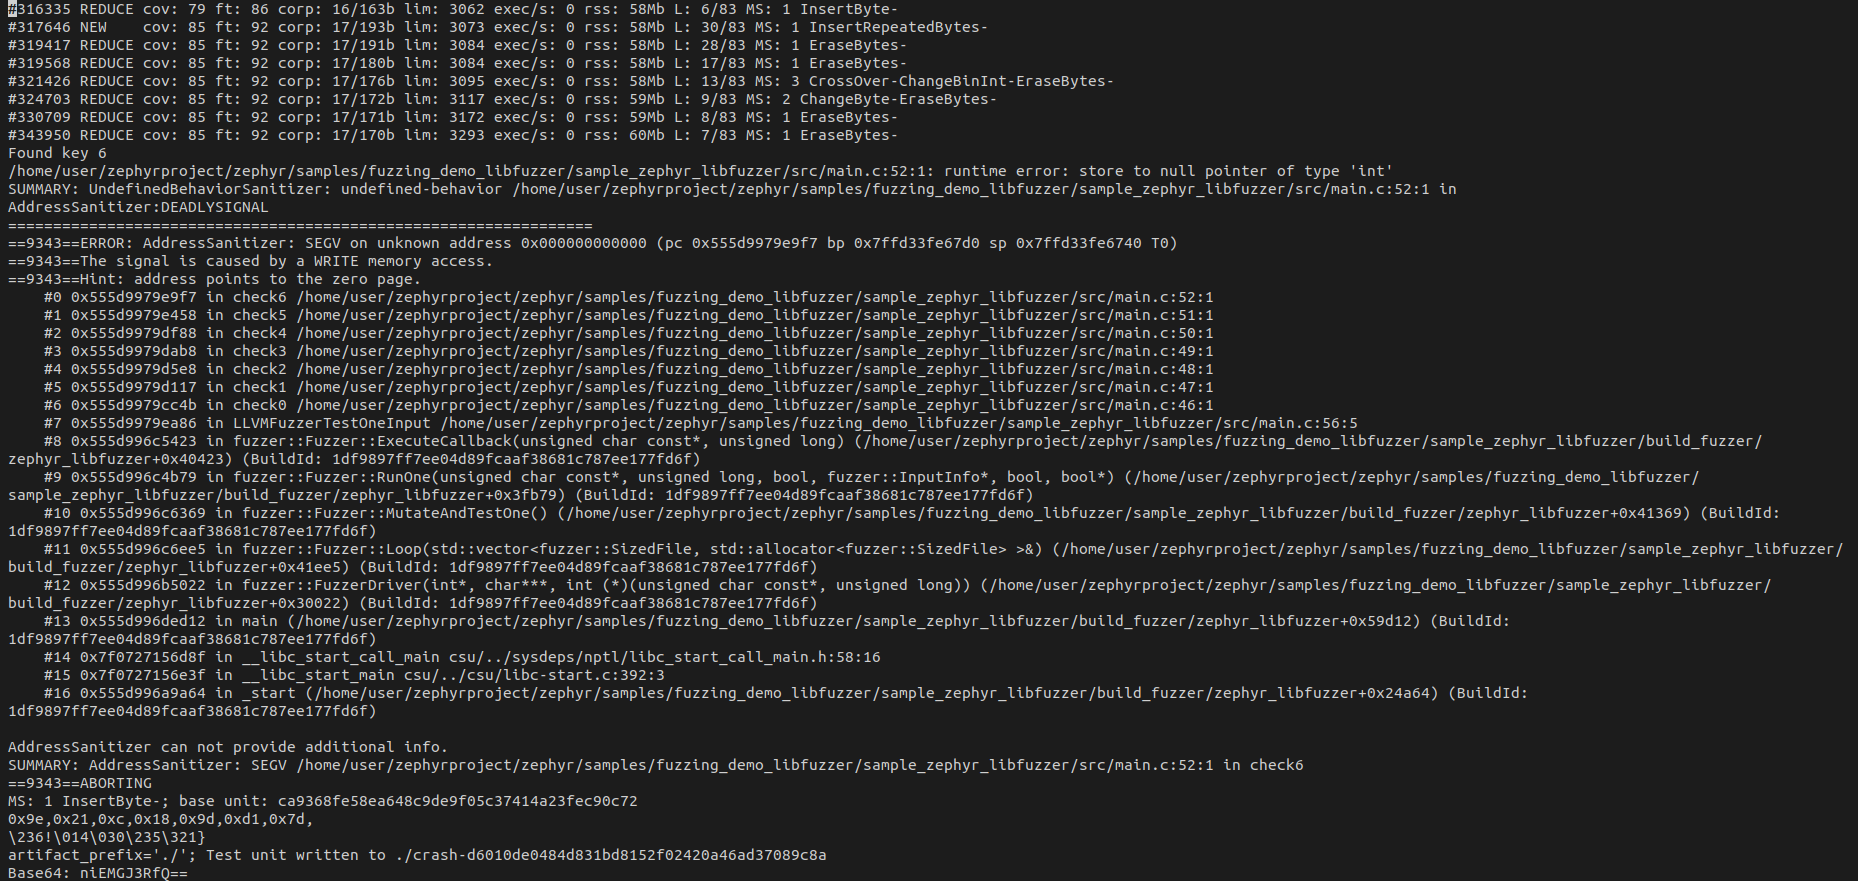
\includegraphics{lib_fuzzer}}
    \caption{libFuzzer Execution Screen}~\label{fig:lib_fuzzer}
\end{figure}
The fuzzer initialized its execution with a specific random seed,
identified as 758034908~\ref{fig:lib_fuzzer}. To reproduce the same
sequence of fuzzing events and outcomes, one may rerun the fuzzer
specifying the argument \texttt{-seed=758034908}.

\begin{minted}[linenos,frame=lines,baselinestretch=1.2,breaklines]{sh}
    INFO: Running with entropic power schedule (0xFF, 100).
    INFO: Seed: 758034908
    INFO: Loaded 1 modules   (157 inline 8-bit counters): 157 [0x555d997e79a8, 0x555d997e7a45),
    INFO: Loaded 1 PC tables (157 PCs): 157 [0x555d997e7a48,0x555d997e8418),
    INFO: -max_len is not provided; libFuzzer will not generate inputs larger than 4096 bytes
    INFO: A corpus is not provided, starting from an empty corpus
\end{minted}

In its default configuration, \texttt{libFuzzer} operates under
the assumption that the input size is constrained to 4096 bytes or less.
To modify this default input size constraint, two potential strategies exist:
the application of the \texttt{-max\_len=N} argument, where \texttt{N} represents
the desired maximum input length, or the initiation of the fuzzer using a
seed corpus that contains non-empty entries. For this \acrlong{poc},
no corpus or input is provided, hence the libFuzzer starts with an empty corpus.

\begin{minted}[linenos,frame=lines,baselinestretch=1.2,breaklines]{sh}
    #330709 REDUCE cov: 85 ft: 92 corp: 17/171b lim: 3172 exec/s: 0 rss: 59Mb L: 8/83 MS: 1 EraseBytes-
    #343950 REDUCE cov: 85 ft: 92 corp: 17/170b lim: 3293 exec/s: 0 rss: 60Mb L: 7/83 MS: 1 EraseBytes-
    Found key 6
    /home/user/zephyrproject/zephyr/samples/fuzzing_demo_libfuzzer/sample_zephyr_libfuzzer/src/main.c:52:1: runtime error: store to null pointer of type 'int'
    SUMMARY: UndefinedBehaviorSanitizer: undefined-behavior /home/user/zephyrproject/zephyr/samples/fuzzing_demo_libfuzzer/sample_zephyr_libfuzzer/src/main.c:52:1 in
    AddressSanitizer:DEADLYSIGNAL
    =================================================================
    ==9343==ERROR: AddressSanitizer: SEGV on unknown address 0x000000000000 (pc 0x555d9979e9f7 bp 0x7ffd33fe67d0 sp 0x7ffd33fe6740 T0)
    ==9343==The signal is caused by a WRITE memory access.
    ==9343==Hint: address points to the zero page.
\end{minted}

During its execution, \texttt{libFuzzer} has processed a minimum of
316,335(\#330709) distinct inputs. From these, it identified 17 unique
inputs with a combined size of 170 bytes (corpus: 17 entries totaling 170 bytes)
that cumulatively achieve coverage over 85 specific points within the target program.

Remarkably, for one particular input, the integrated \texttt{AddressSanitizer}~\cite{GitHubgo55:online}
identified an anomaly characterized as undefined behavior. Consequently, this prompted
the termination of the fuzzer's execution.

Before ending its process, \texttt{libFuzzer} saved the input causing the issue
to the disk. This action guarantees the ability to independently review the
specific conditions that resulted in the problem. Additionally,
it is important to note that the inputs causing crashes are stored in the same
directory to reproduce the issue. To reproduce the observed
behavior without additional fuzzing, execute the command with the input file
the causing the crash such as below:

\begin{minted}[linenos,frame=lines,baselinestretch=1.2,breaklines]{sh}
./zephyr_libfuzzer crash-{the_input_that_cuased_the_crash_saved_in_the_disk}
\end{minted}

To show the profiling data, the following command utilizing \texttt{llvm-profdata} can be employed:

\begin{minted}[linenos,frame=lines,baselinestretch=1.2,breaklines]{sh}
llvm-profdata merge -sparse default.profraw -o default.profdata
\end{minted}

This operation produces the files \texttt{default.profraw} and \texttt{default.profdata}, capturing the consolidated profiling information.

For a terminal-based summary of the coverage, the \texttt{llvm-cov} tool provides a report as follows:

\begin{minted}[linenos,frame=lines,baselinestretch=1.2,breaklines]{sh}
llvm-cov report ./zephyr_libfuzzer -instr-profile=default.profdata
\end{minted}

Additionally, to create a more detailed visualization in HTML format, the
subsequent command can be used:

\begin{minted}[linenos,frame=lines,baselinestretch=1.2,breaklines]{sh}
llvm-cov show ./zephyr_libfuzzer -instr-profile=default.profdata -format=html -output-dir=coverage
\end{minted}

This command generates an HTML report, which can be conveniently reviewed in a web browser,
providing an insightful representation of the code's coverage.

The Figure:~\ref{fig:llvm_cov_report} shows the libFuzzer coverage output in html format.

\begin{figure}[H]
    \adjustbox{width=\textwidth}{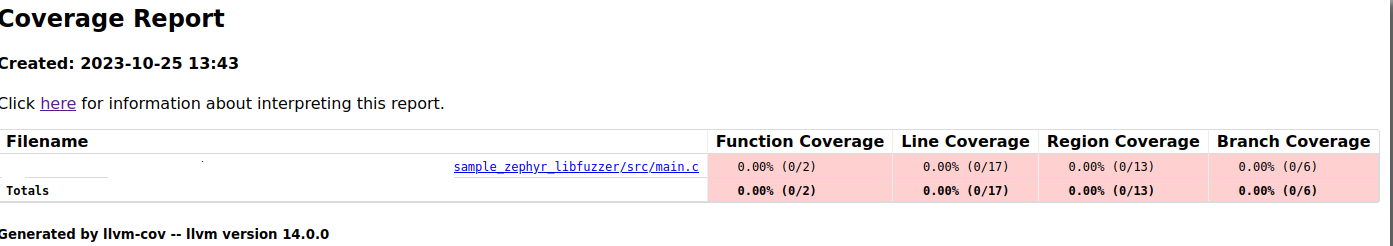
\includegraphics{llvm_cov_report}}
    \caption{libFuzzer Coverage Report}~\label{fig:llvm_cov_report}
\end{figure}

\section{Implementations Using AFL++ QEMU mode}

When conducting vulnerability analyses on closed-source binaries, the
AFL++'s QEMU~\cite{AFLplusp57:online} mode proves invaluable. In the absence of
source code, recompilation to create an instrumented binary is not possible.
AFL++-QEMU~\cite{AFLplusp57:online} addresses this issue through
a specialized version of QEMU's User Mode Emulation~\cite{bellard2005qemu},
facilitating the execution of the original binary while concurrently gathering essential coverage data.
This enhances the efficacy of identifying vulnerabilities within closed-source
binaries.

Steps to start fuzzing with AFL++-QEMU Mode:

\subsection*{Step 1: Identify the Fuzz Target}

The target binary accepts inputs from the host, parses it, and then sends the
data to the application. Given that the binary is closed-source,
the method of instrumentation is unknown.

The Figure:~\ref{fig:simplified_closed_binaries} shows the workflow with the target binary
for the fuzzy testing with AFL++'s QEMU~\cite{AFLplusp57:online} mode.

\begin{figure}[H]
    \adjustbox{width=\textwidth}{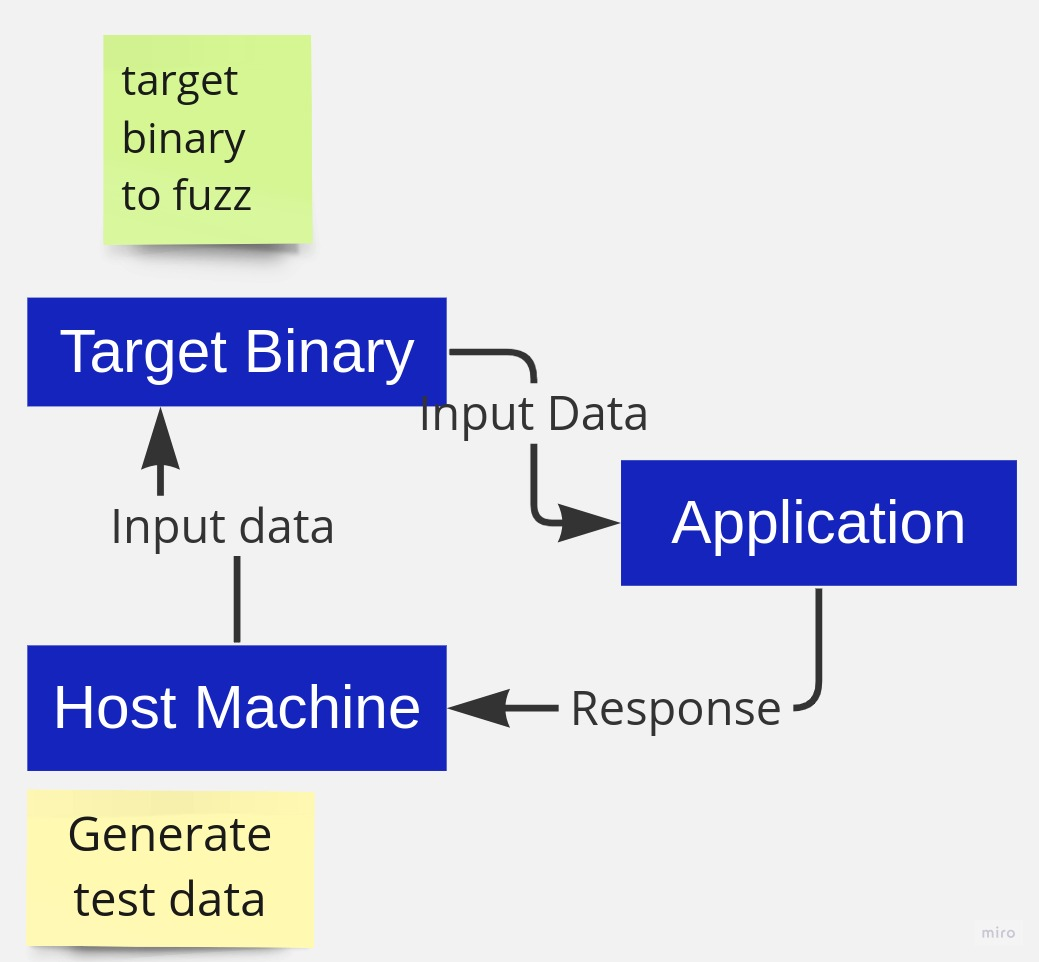
\includegraphics{simplified_closed_binaries}}
    \caption{Closed Source Target Binary}\label{fig:simplified_closed_binaries}
\end{figure}

\subsection*{Step 2: Create Test data}
Generate the initial test data for fuzzing. The test comprises files that
contain various data types. Execute the following command to generate the files:

\begin{minted}[linenos, frame=lines, baselinestretch=1.2, breaklines]{sh}
mkdir input
python3 generate_files.py
\end{minted}

Refer to Appendix~\ref{appx:third} for the script.

\subsection*{Step 3: Docker Script for AFL++-QEMU}
This step is same as that of the~\ref{subsec:docker script for afl-fuzz}.

\begin{minted}[linenos,frame=lines,baselinestretch=1.2,breaklines]{sh}
#!/bin/bash
# Pull the AFL++ Docker image
$ docker pull aflplusplus/aflplusplus
# Run a container using the pulled image
$ docker run -ti -v /home/uname:/home/uname --name afl_container aflplusplus/aflplusplus
# Get into the container
$ docker exec -it afl_container /bin/bash
\end{minted}

\subsection*{Step 5: Fuzzing with AFLL++-QEMU mode, Results, And Analysis}
From the container execute the the below command with
QEMU mode (\begin{math}-Q\end{math} flag)

\begin{minted}{sh}
    $ afl-fuzz -i input/ -o output -Q -- /target_binary param1 param2 @@
\end{minted}

\begin{math}-Q\end{math} flag enables QEMU mode.
\textit{param1} and \textit{param2} are parameters that the target binary requires to run.
They are passed as command-line arguments to the target binary.

The Figure:~\ref{fig:simplified_closed_binaries_qemu} shows the basic
AFL++'s QEMU mode execution.

\begin{figure}[H]
    \adjustbox{width=\textwidth}{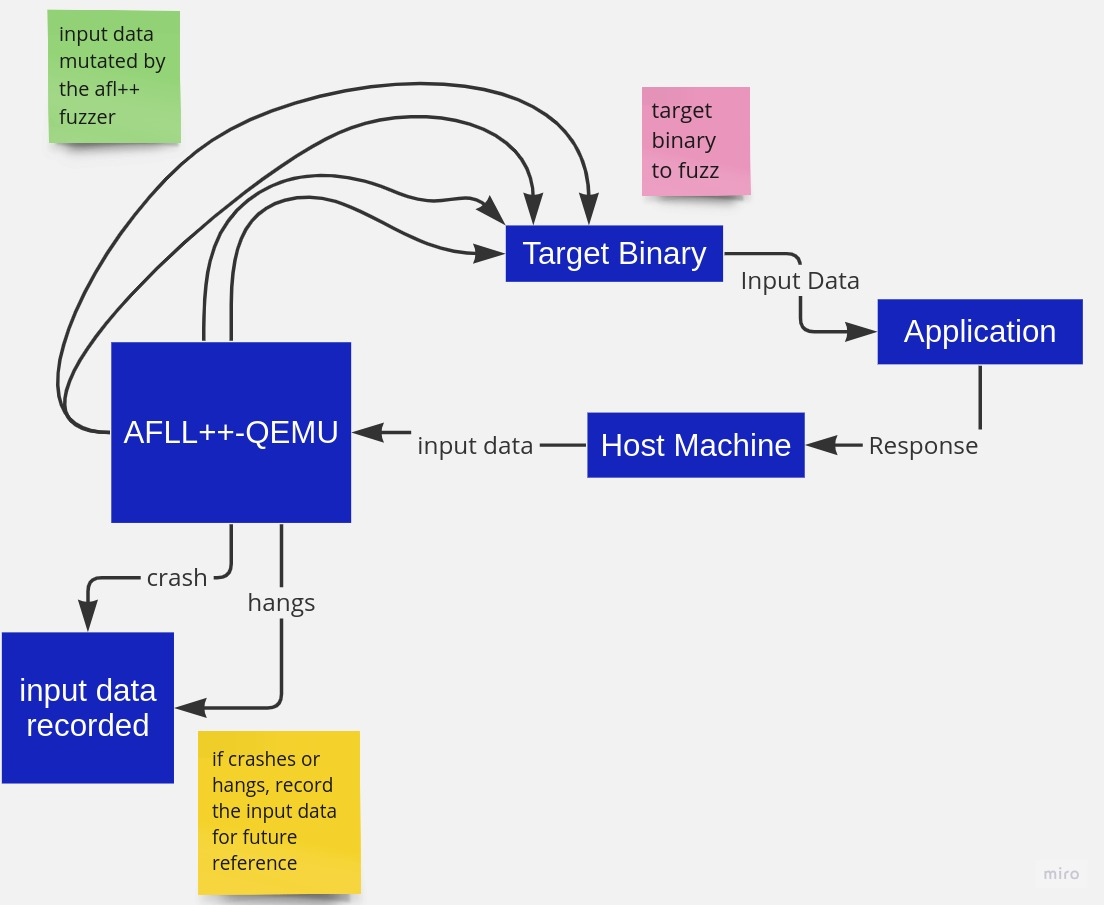
\includegraphics{simplified_closed_binaries_qemu}}
    \caption{Basic AFL++-QEMU Execution }\label{fig:simplified_closed_binaries_qemu}
\end{figure}

The explanation of the execution screen is same that of the~\ref{subsec:execution afl-fuzz}.

The Figure:~\ref{fig:afl_execute_qemu} shows the AFL++-QEMU execution screen.
\begin{figure}[H]
        \adjustbox{width=\textwidth}{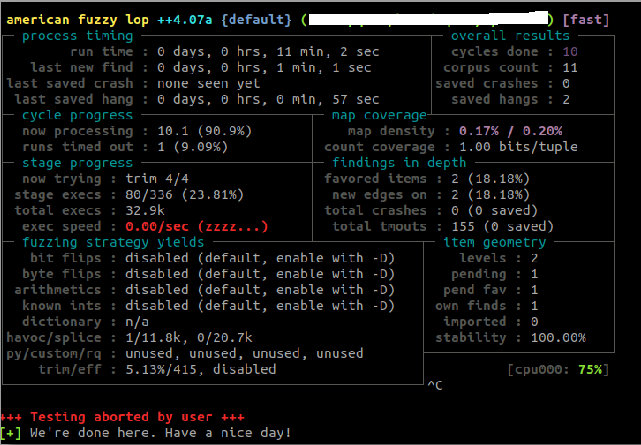
\includegraphics{afl_execute_qemu}}
        \caption{AFL++-QEMU mode Execution Screen}\label{fig:afl_execute_qemu}
\end{figure}


From the execution screen, it was observed that after running the fuzzing
process for 11 minutes, it was forcefully stopped due to receiving 155 timeouts.
There were no crashes, but two hangs were recorded. The inputs causing these
hangs have been saved in the `output/default/hangs/' directory for further
analysis.

While the fuzzer running, `afl-whatsup' is used to show the status.

\begin{minted}{sh}
    $ afl-whatsup -s output
\end{minted}

\begin{minted}[linenos,frame=lines,baselinestretch=1.2,breaklines]{sh}
    Summary stats
    =============
           Fuzzers alive : 1
          Total run time : 11 minutes, 1 seconds
             Total execs : 18 thousands
        Cumulative speed : 27 execs/sec
           Average speed : 27 execs/sec
           Pending items : 0 faves, 0 total
           Crashes saved : 0
    Cycles without finds : 1
      Time without finds : 8 minutes, 23 seconds
\end{minted}

Upon further analysis, the files saved in `output/default/hangs/' were executed
manually against the target binary, but no hangs were observed. This indicates
that there might be a need for additional debugging in both the `afl-fuzz' tool
and the target binary. This area could be explored in future research on the topic
and not in current scope.

\clearpage
% uncomment what you need.
%% Project Specifications

\chapter{Project Specifications}

Check Final Year Project Guide for the content of Project Specifications chapter.

%% Material and Methods

\chapter{Material and Methods}

Check Final Year Project Guide for the content of Material and Methods chapter.

\clearpage %force the next chapter to start on a new page. Keep that as the last line of your chapter!

%% Theoretical background

\chapter{Theoretical background}

Check Final Year Project Guide for the content of Theoretical background chapter.

\clearpage %force the next chapter to start on a new page. Keep that as the last line of your chapter!

%% Proposed solution
%\clearpage%if the chapter heading starts close to bottom of the page, force a line break and remove the vertical vspace
\vspace{21.5pt}
\chapter{Proposed solution}

Check Final Year Project Guide for the content of Proposed solution chapter.

% Conclusions
%\clearpage%if the chapter heading starts close to bottom of the page, force a line break and remove the vertical vspace
\vspace{21.5pt}
\chapter{Discussions and Conclusions}
% Discussions
\section{Discussions}

Fuzzing fulfills a dual role in software testing: it is an effective
preliminary screening method for potential vulnerabilities and a sophisticated
tool for probing complex systems. Its effectiveness is evident in the range of
vulnerabilities it uncovers—some are detected quickly, while others may be more
elusive. However, fuzzing alone cannot guarantee system security; the lack of
discovered bugs does not necessarily indicate invulnerability but may suggest
areas for fuzzer enhancement.

The field of fuzzing is continuously evolving, with the introduction of
innovative open-source fuzzers that enhance broader projects. State-of-the-art
tools such as AFL++, libFuzzer, and Atheris reflect a commitment to continuous
improvement and adaptability.

The incorporation of artificial intelligence into fuzzing
strategies~\cite{GoogleOn27:online} introduces a new level of complexity.
AI-powered tools, utilizing machine learning techniques, strive to create
adaptive testing scenarios and improve vulnerability detection rates,
potentially addressing the traditional limitations of fuzzers.

Reflecting on this exploration of fuzzing, it becomes apparent that fuzzing is
not just a component of software testing but a significant field of study.
Overcoming the challenges of understanding fundamental concepts and managing
complex tool configurations has laid a strong foundation for future research,
which will focus on evaluating various fuzzing approaches in different settings.

Embedded systems pose distinct challenges for fuzzing due to their specialized
nature and operational constraints. The variety of hardware platforms requires
the creation of tailored fuzzing tools that can interact with unique hardware
components and communication protocols. Moreover, the constrained computational
resources in embedded devices limit the scope of extensive fuzzing campaigns.

Proprietary operating systems and software stacks in embedded systems, often
optimized for performance and reliability, lack the necessary debugging and
monitoring tools for effective fuzzing. The real-time operations of many
embedded systems also impose strict timing constraints, further complicating the
fuzzing process.

The physical inaccessibility of many embedded devices complicates the
establishment of fuzzing environments and the iterative cycle of test, debug,
and retest, which is crucial for comprehensive vulnerability assessment.
Consequently, there is a significant need for remote and automated fuzzing
solutions tailored to the unique demands of embedded systems.

\subsection*{Advanced Fuzzing Considerations}

A comparative analysis of the aforementioned fuzzing tools indicates distinct
strengths and optimal use cases for each. AFL++ is renowned for its speed and
user-friendliness, libFuzzer's integration with Sanitizers enables thorough code
analysis, and Atheris excels with Python codebases. A deep understanding of each
tool's capabilities is essential for their effective deployment in securing
software.

Case studies demonstrate the practical impact of fuzzing, yet also reveal its
limitations, underscoring the importance of complementary testing methods. These
real-world examples are invaluable for refining fuzzing techniques and
fortifying software systems.

Economic factors play a critical role in the decision to implement fuzzing as a
security strategy. The initial investment in fuzzing infrastructure and
expertise must be balanced against the long-term benefits of early vulnerability
detection and mitigation.

Integrating fuzzing within DevOps, especially in CI/CD pipelines, offers
promising enhancements to software security by embedding automated checks into
the development cycle.


The human element in fuzzing is irreplaceable; the skill and intuition of
security researchers are vital in steering the fuzzing process and interpreting
its outcomes. Advancements in automated fuzzing aim to complement and, in some
cases, surpass human-led testing efforts.


Looking ahead, the field of fuzzing must adapt to emerging technologies like
quantum computing and develop new methodologies to keep pace with the growing
complexity of software architectures.

\section{Conclusions}

This research highlights the significant potential of fuzzing in the realm of
embedded system software testing. Experiments with libFuzzer and AFL++ have
confirmed their ability to swiftly uncover vulnerabilities. These tools, with
their automated reporting features, simplify the complex task of analyzing code
coverage and identifying potential security weaknesses.

The study advocates for the integration of fuzzing into the standard software
development lifecycle, particularly within continuous testing frameworks. As
software intricacy escalates, the necessity for thorough and efficient testing
processes becomes paramount. The strategic implementation of fuzzing tools
ensures that software is not only functional but also secure against potential
threats.

This thesis provides insights into the current landscape of software testing
and establishes a foundation for future testing strategies. The critical need
for evolving testing methodologies is emphasized, and the empirical evidence
presented serves as a basis for adopting advanced testing approaches.

In conclusion, the domain of fuzzing is dynamic and comprehensive. It offers
substantial benefits for software security but also presents numerous challenges
that must be continually addressed. The progressive development of fuzzing tools
and methods, along with a nuanced understanding of their application, remains
crucial for the future of software testing and security.

% Sample content to demonstrate LaTeX command. You will likely delete this line and the
% next \input{sample/*} lines. You are also safe to delete the sample/ folder and its
% content once you refershed your LaTeX skills. Also check the appendix samples.
% %sample content to demonstrate LaTeX command.
\vspace{21.5pt}
\chapter{Demonstration Content}\label{demo:content}

This is a chapter to demonstrate some of the \gls{latex} commands that you can use to format your text. If you are new to it, \gls{latex} follows the \gls{wysiwym} idea similar to \gls{html} where you concentrate on the content and structure and leave the formatting and styling to the computer. You will write your content in a plain text file\footnote{which can not get corrupted and can be put under version control} and indicate the structure with commands (similar to \gls{html} tags) then compile it to generate the pdf. Check some books or tutorials such as \LaTeX{} Wikibooks\footnote{\url{https://en.wikibooks.org/wiki/LaTeX}} and try with an online editor such as Overleaf\footnote{\url{https://www.overleaf.com/}} so you do not need to install the compiler on your computer first.

\section{Text, terms and abbreviations}

In \gls{latex}, the \mintinline{tex}{\textbf{bold}} command produces \textbf{bold}, \mintinline{tex}{\textit{italic}}  \textit{italic} and nesting \mintinline{tex}{\textbf{\textit{bolditalic}}} generates \textbf{\textit{bolditalic}}. If the goal is to semantically mark importance, then use \emph{emphasize} with \mintinline{tex}{\emph{emphasize}} command. That would take care of cases such as \mintinline{tex}{\textit{text in italic with \emph{important stuff} inside}} which will compile to \textit{text in italic with \emph{important stuff} inside}.

When one want to use an abbreviation or acronym like \gls{html} using the \mintinline{tex}{\gls{html}} command in \gls{latex}, the first time, it comes with it full version as can be seen in first paragraph of chapter \ref{demo:content} and for all next uses in its short form. Of course, when needed, the full version is available using e.g. the \mintinline{tex}{\acrlong{someID}} command. The defined terms like \gls{maths} use the same \mintinline{tex}{\gls{math}} \gls{latex} command. The Capitalized can be obtained with \mintinline{tex}{\Gls{id}}.

In this template, the abbreviations are defined in the \texttt{chapters/0abbr.tex} file with the \mintinline{tex}{\newacronym{id}{SHORT}{Long Form}} command. There can be many abbreviations and terms defined there, only the ones that are used in the text will be printed in the list of abbreviations (after table of content). And of course, it is the job of the compiler to sort them alphabetically. Should be avoided; but to have all the abbreviations and terms, even the non-used ones, use the \mintinline{tex}{\glsaddall} command before printing the list of abbreviations.

\section{Section with references}
Here is an example how to cite a bibliography entry \cite{kopka:guide} using the \textquotedblleft\textbackslash{}cite\textquotedblright ~\gls{latex} command ~\cite[section 4.2]{tobias:book}. You might also like \textquotedblleft\textbackslash{}citeauthor\textquotedblright and \textquotedblleft\textbackslash{}citedate\textquotedblright ~as demonstrated in figure \ref{fig:latex-cover} caption.  Note that a paragraph is added by forcing a new line.

And let also try the figure (see figure \ref{fig:latex-cover}) and internal reference (with ~\textbackslash{}label and ~\textbackslash{}ref). Alternative text is optained with custom made ~\textbackslash{}AltText command (using pdfcomment and accsupp packages). The reference can be done to any label, for example why not to appendix \ref{appx:first} or to appendix \ref{appx:second}? To note, \gls{latex} will place the figure to the best place (except with forcing). Let them float till the final of final edit\ldots ~then force them to not break a paragraph.%hugly hack... I'm sorry
\begin{figure}[ht]
  \centering
  \AltText{meaningful alternative description (e.g. LaTeX, from typeseting to genrated pdf)}{
\includegraphics[width=7.1cm]{LaTeX_cover}}
  \caption{\gls{latex} cover image (Copied from \citeauthor{wikibooks:latex} (\citedate{wikibooks:latex}) \cite{wikibooks:latex}).}
  \label{fig:latex-cover}
\end{figure}

Let's also try a long quote:
From the Universal Declaration of Human Rights:
\begin{quote}
(1) Everyone has the right to education. Education shall be free, at least in the elementary and fundamental stages. Elementary education shall be compulsory. Technical and professional education shall be made generally available and higher education shall be equally accessible to all on the basis of merit.

(2) Education shall be directed to the full development of the human personality and to the strengthening of respect for human rights and fundamental freedoms. It shall promote understanding, tolerance and friendship among all nations, racial or religious groups, and shall further the activities of the United Nations for the maintenance of peace.

(3) Parents have a prior right to choose the kind of education that shall be given to their children. \cite[article 26]{un:udhr}
\end{quote}

\textit{Quisque augue} est, \textbf{elementum ac porttitor} non, porttitor ac orci. Donec hendrerit, ligula ac luctus egestas, sem dolor pretium nunc, sed vehicula magna diam a massa. Donec mattis, arcu et tempor mattis, risus tortor ultrices metus, nec sodales sem dolor eu elit.

\begin{itemize}
  \item Check the guide about the orphan list item: if only first item in the page, force a new page \textbackslash~clearpage before.
  \item When the list items are not sentences, they begin with a lowercase letter, and the last list item ends in a period.
  \item When the list items are sentences, they begin with a capitalized letter, and the list items end in a period. If item of the list contains a long text that spans multiple lines, the left edge aligns automatically.
\end{itemize}

Nullam egestas enim at odio pellentesque bibendum.

\subsection{Subsection}
Donec et sapien ac leo condimentum vulputate id et tellus. Maecenas hendrerit malesuada interdum. Aenean dignissim sem faucibus elit congue faucibus id non risus. Morbi at dui non tortor pellentesque consequat non eget urna. Cras in sapien dui, a tincidunt velit.
\reaction{\label{eq:reaktio}$\underset{\text{+II}}{\ce{2Fe^2+}}$ + $\underset{\text{+I\;-I}}{\ce{H2O2}}$ + $\underset{\text{+I\;-II}}{\ce{2H3O^+}}$ <=> $\underset{\text{+III}}{\ce{2Fe^3+}}$ + $\underset{\text{+I\;-II}}{\ce{4H2O}}$}
Työn aluksi rauta(II)ionit hapetetaan rauta(III)ioneiksi väkevällä vetyperoksidilla, kuten reaktion~\ref{eq:reaktio} hapetusluvuista nähdään (rauta hapettuu, happi pelkistyy).
\reaction{Fe^3+( \emph{aq} ) + 3OH^-( \emph{aq} ) + $(x-1)$H2O( \emph{l} ) -> FeOOH $\cdot$ $x$(H2O)( \emph{s} )}
Rauta(III)ionit saostetaan emäksen (\ce{NH3}) avulla ja saadaan tuotteeksi kidevedellinen rauta(III)hydroksidi. Saatu saostuma pestään \ce{NH4NO3}:lla.
\reaction{FeOOH $\cdot$ $x$(H2O)( \emph{s} ) ->T[$\Delta$900-1000\celsius] Fe2O3( \emph{s} )}

\subsection{Subsection with \texorpdfstring{\Gls{maths}}{Mathematics}}%gls inside chapter/section/... will generate hyperref warning (link inside link in table of content), to avoid that, use the \texorpdfstring
Donec et sapien ac leo condimentum vulputate id et tellus. Maecenas hendrerit malesuada interdum. Aenean dignissim sem faucibus elit congue faucibus id non risus. Morbi at dui non tortor pellentesque consequat non eget urna. Cras in sapien dui, a tincidunt velit. Tertiäärinen butyylikloridi reagoi veden kanssa oheisen reaktion mukaisesti:
\reaction{(CH3)3CCl + 2H2O -> (CH3)3COH+H3O+ +Cl-}
Kyseessä on ensimmäisen kertaluvun reaktio, joten reaktion nopeus on
\begin{align}
v=-\frac{\mathrm{d}[\tn{t-ButCl}]}{\mathrm{d}t}=\frac{\mathrm{d}[\tn{HCl}]}{\mathrm{d}t}=k[\tn{t-ButCl}]
\end{align}
Jos tarkastellaan lähtöaineen t-butyylikloridin häviämistä saadaan
\begin{align}
\frac{\mathrm{d}[\tn{t-ButCl}]}{[\tn{t-ButCl}]}&=-k\mathrm{d}t \\
\int \frac{\mathrm{d}[\tn{t-ButCl}]}{[\tn{t-ButCl}]}&=-k \int \mathrm{d}t \\
\ln \int_{[\tn{t-ButCl}]_0}^{[\tn{t-ButCl}]} [\tn{t-ButCl}]&=-k\int_0^t t \\
\ln \left( \frac{[\tn{t-ButCl}]}{[\tn{t-ButCl}]_0} \right)&=-kt
\end{align}
Ionivahvuus lasketaan kaavalla.
\begin{align}
I&=\frac{1}{2}\cdot\sum z_i^2c_i \\
z_i&= \tn{ionin varausluku} \nonumber \\
c_i&= \tn{ionin konsentraatio} \nonumber
\end{align}
Aktiivisuuskerroin $\gamma_\pm$ lasketaan kaavalla.
\begin{align}
\log \gamma_\pm &= -\left|z_+\cdot z_-\right|A\cdot I^{\frac{1}{2}} \\
A &= \tn{0,509 (lämpötilassa 25\celsius}) \nonumber \\
I &= \tn{ionivahvuus} \nonumber \\
z &= \tn{ionien varaus} \nonumber
\end{align}

\section{Section with Source Code}
Donec et sapien ac leo condimentum vulputate id et tellus. Maecenas hendrerit malesuada interdum. Aenean dignissim sem faucibus elit congue faucibus id non risus. Morbi at dui non tortor pellentesque consequat non eget urna. Cras in sapien dui, a tincidunt velit.

%For sharelatex users, use space instead of tab to avoid ^^I
\begin{code}
  \begin{minted}{php}
<?php
$username = $_POST["username"];
//maybe not?
if ($userName){
  ?>
  <h2>Hello <?= $username ?>!</h2>
  <p>your message got received.</p>
  <?php
}
?>
\end{minted}
\captionof{listing}{Descriptive Caption Text (e.g. this \gls{php} code do blah)}
  \label{code:testphp}
\end{code}


As see in listing \ref{code:testphp}, blah. It is also possible to have code inline, for example \mintinline{sql}{SELECT * FROM user WHERE age >= 18} that was \gls{sql}.
The lisings \ref{code:htmlfull} and \ref{code:htmlpart} show how to load code from an external source file. In the case of listing \ref{code:htmlpart} it only take few line out of the source code file.

\begin{code}
  \inputminted{html}{code/html5_sample.html}
  \captionof{listing}{Some \gls{html} code}
  \label{code:htmlfull}
\end{code}
 Donec et sapien ac leo condimentum vulputate id et tellus. Maecenas hendrerit malesuada interdum. Aenean dignissim sem faucibus elit congue faucibus id non risus.

 \begin{code}
   \inputminted[firstline=3,lastline=6]{html}{code/html5_sample.html}
   \captionof{listing}{The \mintinline{html}{<head>} section of an \gls{html} page}
  \label{code:htmlpart}
\end{code}


 Morbi at dui non tortor pellentesque consequat non eget urna. Cras in sapien dui, a tincidunt velit.


\section{Section with Table}
Donec et sapien ac leo condimentum vulputate id et tellus. Maecenas hendrerit malesuada interdum. Aenean dignissim sem faucibus elit congue faucibus id non risus. Morbi at dui non tortor pellentesque consequat non eget urna. Cras in sapien dui, a tincidunt velit.

\begin{table}[h]
  \centering
  \caption{Some data}%IMPORTANT the caption must be before the tabular, so it will be on top of the table (there are other tricks to force it on top; but this one is straightforward).
  \vspace{-16.5pt}%time to time, spacing between caption and table can go too big...
  \begin{tabular}{| l | >{\centering\arraybackslash}p{.5\textwidth} |}
    \hline
    Test 1 & test 1234 test \\
    \hline
    Some more data comes here & with more values and if the text is very long it will disappear out of the box unless you force the column size :( You can use e.g. \textbackslash raggedright or \textbackslash centering (as in this example) to avoid hyphenization of long words\ldots \\
    \hline
  \end{tabular}
  \label{table:some_data}
\end{table}

As presented in table \ref{table:some_data}: Donec et sapien ac leo condimentum vulputate id et tellus. Maecenas hendrerit malesuada interdum. Aenean dignissim sem faucibus elit congue faucibus id non risus. Morbi at dui non tortor pellentesque consequat non eget urna. Cras in sapien dui, a tincidunt velit.

\begin{table}[h]
  \centering
  \caption{Another table with tabularx}
  \begin{tabularx}{.95\textwidth}{| l | >{\centering\arraybackslash} X |}
    \hline
    Test 1 & test 1234 test \\
    \hline
    Some more data comes here & with more values and if the text is very long it will disappear out of the box unless you force the table size :( \\
    \hline
  \end{tabularx}
  \label{table:some_data2}
\end{table}

As presented in table \ref{table:some_data2}: Donec et sapien ac leo condimentum vulputate id et tellus. Maecenas hendrerit malesuada interdum. Aenean dignissim sem faucibus elit congue faucibus id non risus. Morbi at dui non tortor pellentesque consequat non eget urna. Cras in sapien dui, a tincidunt velit.

Donec et sapien ac leo condimentum vulputate id et tellus. Maecenas hendrerit malesuada interdum. Aenean dignissim sem faucibus elit congue faucibus id non risus. Morbi at dui non tortor pellentesque consequat non eget urna. Cras in sapien dui, a tincidunt velit.

\begin{table}[htbp]
  \centering
  \caption{Booktabs example}
  \vspace{-16.5pt}
    \begin{tabular}{rrrr}
    \toprule
    t (s) & [HCl] & [t-ButCl] & $\ln\frac{[t-ButCl]}{[t-ButCl]_0}$ \\
    \midrule
    0     & 4,02  & 160,88 & 0,00 \\
    10    & 63    & 101,9 & -0,46 \\
    20    & 115,2 & 49,7  & -1,17 \\
    30    & 141,3 & 23,6  & -1,92 \\
    40    & 157,9 & 7     & -3,13 \\
    50    & 161   & 3,9   & -3,72 \\
    60    & 164,3 & 0,6   & -5,59 \\
    70    & 163,5 & 1,4   & -4,74 \\
    80    & 163,8 & 1,1   & -4,99 \\
    90    & 164,1 & 0,8   & -5,30 \\
    100   & 164,3 & 0,6   & -5,59 \\
    \bottomrule
    \end{tabular}
  \label{tab:thisislabel}
\end{table}

As presented in table \ref{tab:thisislabel}: Donec et sapien ac leo condimentum vulputate id et tellus. Maecenas hendrerit malesuada interdum. Aenean dignissim sem faucibus elit congue faucibus id non risus. Morbi at dui non tortor pellentesque consequat non eget urna. Cras in sapien dui, a tincidunt velit.

% %Dummy content to use some space...

\chapter{Dummy Content}

Lorem ipsum dolor sit amet, consectetur adipiscing elit. Aliquam aliquam aliquam purus, in ornare nulla imperdiet molestie. Nam tempus erat eu dui rhoncus et vestibulum mi elementum. Ut porttitor elit sit amet justo dignissim sit amet sagittis massa egestas. Mauris sed dolor eget dui fermentum sodales ut eu nibh. 

Quisque augue est, elementum ac porttitor non, porttitor ac orci. Donec hendrerit, ligula ac luctus egestas, sem dolor pretium nunc, sed vehicula magna diam a massa. Donec mattis, arcu et tempor mattis, risus tortor ultrices metus, nec sodales sem dolor eu elit. Nullam egestas enim at odio pellentesque bibendum. 

Donec et sapien ac leo condimentum vulputate id et tellus. Maecenas hendrerit malesuada interdum. Aenean dignissim sem faucibus elit congue faucibus id non risus. Morbi at dui non tortor pellentesque consequat non eget urna. Cras in sapien dui, a tincidunt velit.

\clearpage %force the next chapter to start on a new page. Keep that as the last line of your chapter!

% % Sample content to demonstrate tikzpicture

\chapter{Graph}

Lorem ipsum dolor sit amet, consectetur adipiscing elit. Aliquam aliquam aliquam purus, in ornare nulla imperdiet molestie. Nam tempus erat eu dui rhoncus et vestibulum mi elementum. Ut porttitor elit sit amet justo dignissim sit amet sagittis massa egestas. Mauris sed dolor eget dui fermentum sodales ut eu nibh.
\begin{figure}[htbp]
  \centering
    \begin{tikzpicture}
        \pgfplotsset{width=12cm,
        compat=1.3,
        legend style={font=\footnotesize}}
    \begin{axis}[
    xlabel={c (mg/l)},
    ylabel={A},
    legend pos=north west,
    ymajorgrids=true,
    grid style=dashed
]

\addplot [only marks, blue] table {data.dat};
\addplot [no markers, thick, red] table[
x=c,
y={create col/linear regression}] {data.dat};
\addlegendentry{data}
\addlegendentry{%
$\pgfmathprintnumber{\pgfplotstableregressiona}x
\pgfmathprintnumber[print sign]{\pgfplotstableregressionb}$}
\end{axis}
\end{tikzpicture}
\label{fig:stdplot}
\caption{Simple linear regression plot (cannot get $r^2$ value)}
\end{figure}

Quisque augue est, as seen in figure \ref{fig:stdplot} elementum ac porttitor non, porttitor ac orci. Donec hendrerit, ligula ac luctus egestas, sem dolor pretium nunc, sed vehicula magna diam a massa. Donec mattis, arcu et tempor mattis, risus tortor ultrices metus, nec sodales sem dolor eu elit. Nullam egestas enim at odio pellentesque bibendum. 

Donec et sapien ac leo condimentum vulputate id et tellus. Maecenas hendrerit malesuada interdum. Aenean dignissim sem faucibus elit congue faucibus id non risus. Morbi at dui non tortor pellentesque consequat non eget urna. Cras in sapien dui, a tincidunt velit.

\section{Section}

Lorem ipsum dolor sit amet, consectetur adipiscing elit. Aliquam aliquam aliquam purus, in ornare nulla imperdiet molestie. Nam tempus erat eu dui rhoncus et vestibulum mi elementum. 
\tikzstyle{palikka} = [rectangle, rounded corners, minimum width=1cm, minimum height=1cm, text centered, text width=2cm, draw=black, fill=red!30]
\tikzstyle{arrow} = [thick,->,>=stealth]
\begin{figure}[htbp]
\centering
\begin{tikzpicture}[node distance=2.75cm]
\node[label=90:Label] (yksi) [palikka] {Lorem};
\node (kaksi) [palikka, right of=yksi] {ipsum};
\node (kolme) [palikka, below of=kaksi,  yshift=1cm] {dolor};
\node (neljä) [palikka, left of=kolme] {sit};
\node (viisi) [palikka, below of=neljä, yshift=1cm] {amet};
\draw [arrow] (yksi) -- (kaksi);
\draw [arrow] (kaksi) -- node[anchor=west] {tekstiä} (kolme);
\draw [arrow] (kolme) -- (neljä);
\draw [arrow] (neljä) -- (viisi);
\end{tikzpicture}
\caption{Example tikz-picture}
\label{fig:tikz}
\end{figure}

As seen in figure \ref{fig:tikz}, ut porttitor elit sit amet justo dignissim sit amet sagittis massa egestas. Mauris sed dolor eget dui fermentum sodales ut eu nibh. 

\section{Section}

Lorem ipsum dolor sit amet, consectetur adipiscing elit. Aliquam aliquam aliquam purus, in ornare nulla imperdiet molestie. Nam tempus erat eu dui rhoncus et vestibulum mi elementum. Ut porttitor elit sit amet justo dignissim sit amet sagittis massa egestas. Mauris sed dolor eget dui fermentum sodales ut eu nibh. 

\clearpage %force the next chapter to start on a new page. Keep that as the last line of your chapter!


%----------------------------------------------------------------------------------------
%	BIBLIOGRAPHY REFERENCES
%----------------------------------------------------------------------------------------

% Bibliography.
% Normally you do not edit this file.
% To add bibliography in your text, add them first in the biblio.bib file and
% reference them with the \cite{} command in your text. Check also \citeauthor
% and \citeyear (e.g. for copied figure caption), the \cites for multi-cites
% with page numbers,...

\clearpage
%line space
%\singlespacing %removed otherwise the appendix are also single space
\begin{flushleft}
\begin{singlespacing}
\printbibliography[title=\IfLanguageName{finnish}{Lähteet}{References}]
\end{singlespacing}
\end{flushleft}

%for conting the pages
\label{LastPage}~

%avoid that the last page of bib get appendix header
\clearpage



%----------------------------------------------------------------------------------------
%	APPENDICES
%----------------------------------------------------------------------------------------
% Appendix
% Normally, you do not have to edit this file.

%start appendix
\appendix
%no page number for appendix in table of content
\addtocontents{toc}{\cftpagenumbersoff{chapter}}
%appendix sections and subsections not in table of content
\settocdepth{chapter}
%add "Appendices" in the table of content
\addappheadtotoc
%have Appendix 1 (instead of Appendix A)
\renewcommand{\thechapter}{\arabic{chapter}} 

\newcommand\liite[1]{
%each appendix restart page num to one
\setcounter{page}{1}
%special counter for appendix TODO: this is a ugly quick hack :( Should find a better way to count the page per appendix.
\newtotcounter{appx#1}
%overwrite the header
\makeevenhead{plain}{}{}{\appname \thechapter \\ \thepage\,(\stepcounter{appx#1}\total{appx#1})}
\makeoddhead{plain}{}{}{\appname \thechapter \\ \thepage\,(\stepcounter{appx#1}\total{appx#1})}}



%force smaller vertical spacing in table of content
%!!! There can be some fun depending if the appendices have (sub)sections or not :D
% You will have to play with these numbers and eventually add the \vspace line  before
% some \chapter and force another number.
% To add more fun, time to time the table of content get wrong after a build :(
\addtocontents{toc}{\vspace{11pt}}
\pretocmd{\chapter}{\addtocontents{toc}{\protect\vspace{-24pt}}}{}{}

\liite{1}% This is a hack to have right page numbering for each appendix. Make sure to
% use a unique number for each appendix.
% Appendix
% And demonstrate text references and bibliography references in appendix

\chapter{AFL++ Target Program}\label{appx:first}
The following is the detailed implementation of the
target program\cite{FuzzingE54:online}\cite{zephyrsa35:online} used in
the fuzz testing with Zephyr apps by utilizing the AFL++\cite{257204}:

\section*{main.c}
\begin{minted}[linenos,frame=lines,baselinestretch=1.2,breaklines]{c}
#include <stdio.h>
#include <stdbool.h>
#include <stdint.h>
#include <stdlib.h>

/* Fuzz testing is coverage-based, so we want to hide a failure case
 * (a write through a null pointer in this case) down inside a call
 * tree in such a way that it would be very unlikely to be found by
 * randomly-selected input.  But the fuzzer can still find it in
 * linear(-ish) time by discovering each new function along the way
 * and then probing that new space.  The 1 in 2^56 case here would
 * require months-to-years of work for a large datacenter, but the
 * fuzzer gets it in 20 seconds or so. This requires that the code for
 * each case be distinguishable/instrumentable though, which is why we
 * generate the recursive handler functions this way and disable
 * inlining to prevent optimization.
 *
 * https://github.com/zephyrproject-rtos/zephyr/blob/main/samples/subsys/debug/fuzz/src/main.c
 */

int *global_null_ptr;

// crash
static const uint8_t key[] = { 0x9e, 0x21, 0x0c, 0x18, 0x9d, 0xd1, 0x7d };
bool found[sizeof(key)/sizeof(key[0])];

#define LASTKEY (sizeof(key)/sizeof(key[0]) - 1)

#define GEN_CHECK(cur, nxt)                           \
    void check##nxt(uint8_t *data, size_t sz);        \
    void check##cur(uint8_t *data, size_t sz)         \
    {                                                 \
        if (cur < sz && data[cur] == key[cur]) {      \
            if (!found[cur]) {                        \
                printf("Found key %d\n", cur);        \
                found[cur] = true;                    \
            }                                         \
            if (cur == LASTKEY) {                     \
                *global_null_ptr = 0; /* boom! */     \
            } else {                                  \
                check##nxt(data, sz);                 \
            }                                         \
        }                                             \
    }

GEN_CHECK(0, 1)
GEN_CHECK(1, 2)
GEN_CHECK(2, 3)
GEN_CHECK(3, 4)
GEN_CHECK(4, 5)
GEN_CHECK(5, 6)
GEN_CHECK(6, 0)


int main(int argc, char **argv)
{
    /*Matches key
    causes crash*/
    //uint8_t test_data[] = { 0x9e, 0x21, 0x0c, 0x18, 0x9d, 0xd1, 0x7d };
    // no crash
    //uint8_t test_data[] = { 0x9e, 0x21, 0x0c, 0x18, 0x9d, 0xd1, 0x7e };
    // Open the file
   if (argc != 2) {
        printf("Usage: %s <input_file>\n", argv[0]);
        return 1;
    }

    // Open the file
    FILE *file = fopen(argv[1], "rb");
    if (file == NULL) {
        printf("Could not open file %s\n", argv[1]);
        return 1;
    }

    // Determine the size of the file
    fseek(file, 0, SEEK_END);
    size_t size = ftell(file);
    fseek(file, 0, SEEK_SET);

    // Allocate memory for the data
    uint8_t *test_data = malloc(size);
    if (test_data == NULL) {
        printf("Could not allocate memory for test data\n");
        fclose(file);
        return 1;
    }

    // Read the data from the file
    if (fread(test_data, 1, size, file) != size) {
        printf("Error reading file %s\n", argv[1]);
        free(test_data);
        fclose(file);
        return 1;
    }

    // Close the file
    fclose(file);

    // Use the data
    check0(test_data, size);

    // Clean up
    free(test_data);
    return 0;
}

\end{minted}

\section*{CMakeLists.txt}
\begin{minted}{cmake}
    cmake_minimum_required(VERSION 3.20.0)
    project(sample_zephyr_afl)

    option(USE_AFL "Use afl" OFF)

    if(USE_AFL)
        set(CMAKE_C_COMPILER afl-gcc-fast)
        set(CMAKE_C_FLAGS "${CMAKE_C_FLAGS} -g -fpic -fprofile-arcs -ftest-coverage")
    else()
        set(CMAKE_C_COMPILER gcc)
    endif()

    add_executable(zephyr_aflfuzzer src/main.c)
    \end{minted}

\clearpage% Sample content to demonstrate appendix in LaTeX. You
% are safe to delete this lines (and the next samples) once you refreshed your LaTeX
% skills (and safe to delete the sample folder and all its file too).
% Appendix
% Just to have more appendices and more content

\chapter{Dummy Appendix}\label{appx:second}

Lorem ipsum dolor sit amet, consectetur adipiscing elit. Aliquam aliquam aliquam purus, in ornare nulla imperdiet molestie. Nam tempus erat eu dui rhoncus et vestibulum mi elementum. Ut porttitor elit sit amet justo dignissim sit amet sagittis massa egestas. Mauris sed dolor eget dui fermentum sodales ut eu nibh.

Quisque augue est, elementum ac porttitor non, porttitor ac orci. Donec hendrerit, ligula ac luctus egestas, sem dolor pretium nunc, sed vehicula magna diam a massa. Donec mattis, arcu et tempor mattis, risus tortor ultrices metus, nec sodales sem dolor eu elit. Nullam egestas enim at odio pellentesque bibendum. 

Donec et sapien ac leo condimentum vulputate id et tellus. Maecenas hendrerit malesuada interdum. Aenean dignissim sem faucibus elit congue faucibus id non risus. Morbi at dui non tortor pellentesque consequat non eget urna. Cras in sapien dui, a tincidunt velit.

Lorem ipsum dolor sit amet, consectetur adipiscing elit. Aliquam aliquam aliquam purus, in ornare nulla imperdiet molestie. Nam tempus erat eu dui rhoncus et vestibulum mi elementum. Ut porttitor elit sit amet justo dignissim sit amet sagittis massa egestas. Mauris sed dolor eget dui fermentum sodales ut eu nibh.

Quisque augue est, elementum ac porttitor non, porttitor ac orci. Donec hendrerit, ligula ac luctus egestas, sem dolor pretium nunc, sed vehicula magna diam a massa. Donec mattis, arcu et tempor mattis, risus tortor ultrices metus, nec sodales sem dolor eu elit. Nullam egestas enim at odio pellentesque bibendum. 

Donec et sapien ac leo condimentum vulputate id et tellus. Maecenas hendrerit malesuada interdum. Aenean dignissim sem faucibus elit congue faucibus id non risus. Morbi at dui non tortor pellentesque consequat non eget urna. Cras in sapien dui, a tincidunt velit.

Lorem ipsum dolor sit amet, consectetur adipiscing elit. Aliquam aliquam aliquam purus, in ornare nulla imperdiet molestie. Nam tempus erat eu dui rhoncus et vestibulum mi elementum. Ut porttitor elit sit amet justo dignissim sit amet sagittis massa egestas. Mauris sed dolor eget dui fermentum sodales ut eu nibh.

Quisque augue est, elementum ac porttitor non, porttitor ac orci. Donec hendrerit, ligula ac luctus egestas, sem dolor pretium nunc, sed vehicula magna diam a massa. Donec mattis, arcu et tempor mattis, risus tortor ultrices metus, nec sodales sem dolor eu elit. Nullam egestas enim at odio pellentesque bibendum. 

Donec et sapien ac leo condimentum vulputate id et tellus. Maecenas hendrerit malesuada interdum. Aenean dignissim sem faucibus elit congue faucibus id non risus. Morbi at dui non tortor pellentesque consequat non eget urna. Cras in sapien dui, a tincidunt velit.

Lorem ipsum dolor sit amet, consectetur adipiscing elit. Aliquam aliquam aliquam purus, in ornare nulla imperdiet molestie. Nam tempus erat eu dui rhoncus et vestibulum mi elementum. Ut porttitor elit sit amet justo dignissim sit amet sagittis massa egestas. Mauris sed dolor eget dui fermentum sodales ut eu nibh.

Quisque augue est, elementum ac porttitor non, porttitor ac orci. Donec hendrerit, ligula ac luctus egestas, sem dolor pretium nunc, sed vehicula magna diam a massa. Donec mattis, arcu et tempor mattis, risus tortor ultrices metus, nec sodales sem dolor eu elit. Nullam egestas enim at odio pellentesque bibendum. 

Donec et sapien ac leo condimentum vulputate id et tellus. Maecenas hendrerit malesuada interdum. Aenean dignissim sem faucibus elit congue faucibus id non risus. Morbi at dui non tortor pellentesque consequat non eget urna. Cras in sapien dui, a tincidunt velit.

Lorem ipsum dolor sit amet, consectetur adipiscing elit. Aliquam aliquam aliquam purus, in ornare nulla imperdiet molestie. Nam tempus erat eu dui rhoncus et vestibulum mi elementum. Ut porttitor elit sit amet justo dignissim sit amet sagittis massa egestas. Mauris sed dolor eget dui fermentum sodales ut eu nibh.

Quisque augue est, elementum ac porttitor non, porttitor ac orci. Donec hendrerit, ligula ac luctus egestas, sem dolor pretium nunc, sed vehicula magna diam a massa. Donec mattis, arcu et tempor mattis, risus tortor ultrices metus, nec sodales sem dolor eu elit. Nullam egestas enim at odio pellentesque bibendum. 

Donec et sapien ac leo condimentum vulputate id et tellus. Maecenas hendrerit malesuada interdum. Aenean dignissim sem faucibus elit congue faucibus id non risus. Morbi at dui non tortor pellentesque consequat non eget urna. Cras in sapien dui, a tincidunt velit.

Lorem ipsum dolor sit amet, consectetur adipiscing elit. Aliquam aliquam aliquam purus, in ornare nulla imperdiet molestie. Nam tempus erat eu dui rhoncus et vestibulum mi elementum. Ut porttitor elit sit amet justo dignissim sit amet sagittis massa egestas. Mauris sed dolor eget dui fermentum sodales ut eu nibh.

Quisque augue est, elementum ac porttitor non, porttitor ac orci. Donec hendrerit, ligula ac luctus egestas, sem dolor pretium nunc, sed vehicula magna diam a massa. Donec mattis, arcu et tempor mattis, risus tortor ultrices metus, nec sodales sem dolor eu elit. Nullam egestas enim at odio pellentesque bibendum. 

Donec et sapien ac leo condimentum vulputate id et tellus. Maecenas hendrerit malesuada interdum. Aenean dignissim sem faucibus elit congue faucibus id non risus. Morbi at dui non tortor pellentesque consequat non eget urna. Cras in sapien dui, a tincidunt velit.


\clearpage %force the next appendix to start on a new page. Keep that as the last line of your appendix!


% % Appendix
% % And demonstrate text references and bibliography references in appendix


\chapter{Test Data Creation for AFL++-QEMU mode}\label{appx:third}
The following python program to create test data for AFL++-QEMU mode.

\section*{generate\_files.py}
\begin{minted}{python}
import os
import random
import secrets
import struct

# Number of files to generate
num_files = 10

# Size of the buffer in bytes
buffer_size = 1024

for i in range(num_files):

    # Generate a random integer
    random_int = random.randint(-2147483648, 2147483647)
    int_str = str(random_int)

    # Generate a random float
    random_float = random.uniform(-1e5, 1e5)
    float_str = f"{random_float:.2f}"

    # Generate a random string
    random_string = secrets.token_urlsafe(random.randint(1, 50))

    # Generate random bytes
    random_bytes = os.urandom(random.randint(1, 50))

    # Generate a random boolean
    random_bool = random.choice([True, False])
    bool_str = str(random_bool)

    # Combine all data into one string
    combined_data = f"{int_str}\n{float_str}\n{random_string}\n{random_bytes}\n{bool_str}\n".encode('utf-8')

    # Check buffer size and truncate if necessary
    if len(combined_data) > buffer_size:
        combined_data = combined_data[:buffer_size]

    # Create a file and write the data to it
    with open(f"input/file_{i}.bin", "wb") as f:
        f.write(combined_data)

\end{minted}

%\clearpage

% BSD change
%\setlength{\footskip}{25pt}
%----------------------------------------------------------------------------------------
%	THIS IS THE END
%----------------------------------------------------------------------------------------
\end{document}
